\chapter{Machine learning analysis implementation}
\label{sec:MLanalysis}

For both machine learning algorithms we have done a few preselection cuts on my data to make our datasets smaller and get a more efficient training time. The cuts we have applied for the four processes is given in table \ref{tab:precutsSlepSlep} below.

\begin{table}[H]
    \centering
    \renewcommand{\arraystretch}{1.}
    \begin{tabular}{c}
    \toprule
    \textbf{Precuts}\\
    \midrule
    \midrule
        \# leptons = 2 \\
        Charge(lep$_1$ $\neq$ lep$_2$)\\
        b-jets = 0\\
        $E_T^{miss}$ $>$ 40 GeV\\
        \bottomrule
    \end{tabular}
    \caption{A table of the precuts we have done before sending the data into the BDT and NN.}
    \label{tab:precutsSlepSlep}
\end{table}

In addition we have selected some different variables in our nTuples\footnote{nTuples are the files we fetch our trees from, which again are the ROOT histograms for each variable in the different samples (data, background and signal) we are looking at.} for the features to train our ML algorithms which are listed up in table \ref{tab:features}.

\begin{table}[H]
    \centering
    \renewcommand{\arraystretch}{1.}
    \begin{tabular}{c c}
    \toprule
    \textbf{Low level features} & \textbf{High level features}\\
    \midrule
    \midrule
        lep $p_{T_1}$ & mll\\
        lep $p_{T_2}$ & mt2\\
        lep $\eta_1$ & $H_T$\\
        lep $\eta_2$ & $E_T^{\text{miss}}/H_T$\\
        lep $\phi_1$ & $\Delta \phi(\Vec{p}_T^{ll}, E_T^{\text{miss}})$\\
        lep $\phi_2$ & $\Delta R_{ll}$\\
        nJet20 & Fractional $p_T$ difference\\
        nJet30\\
        n$_{\text{b-tagged jets}}$\\
        $E_T^{\text{miss}}$\\
        $E_T^{\text{miss}}$ significance\\
        \bottomrule
    \end{tabular}
    \caption{List of features chosen for the training of the ML model.}
    \label{tab:features}
\end{table}

We have also included some different variables to weight each event which is listed up in table \ref{tab:eventWeights}.

\begin{table}[H]
    \centering
    \renewcommand{\arraystretch}{1.}
    \begin{tabular}{c}
    \toprule
    \textbf{Weights}\\
    \midrule
    \midrule
        event weight  \\
        pileup weight \\
        b-tag weight \\
        gen weight \\
        jvt weights (jet vertex tagger)\\
        global dilepton trigger SF (same flavor)\\
        Luminosity for MC 2015-2016 = 36.2 fb$^{-1}$\\
        Luminosity for MC 2017 = 44.3 fb$^{-1}$\\
        Luminosity for MC 2018 = 58.5 fb$^{-1}$\\
        \bottomrule
    \end{tabular}
    \caption{List of weights to weight each event in the dataframes and the luminosity for the data taken in 2015-2018.}
    \label{tab:eventWeights}
\end{table}

We can also see how the different variables/features behave with the ML precuts in the cut and count method. This is shown in figure \ref{fig:ML_cuts} and is shown to see how the different variables behave and is only shown for the direct slepton production process. 

%Change top margin 
\newgeometry{top=20mm, bottom=25mm, twoside,inner=3cm,outer=2cm}
\begin{figure}[H]
%\begin{minipage}{2\textwidth}
%\begin{adjustwidth}{-3cm}{-3cm}
\centering
%\advance\leftskip-4cm 
%\advance\rightskip-4cm 
    \begin{subfigure}[t!]{0.49\textwidth}
        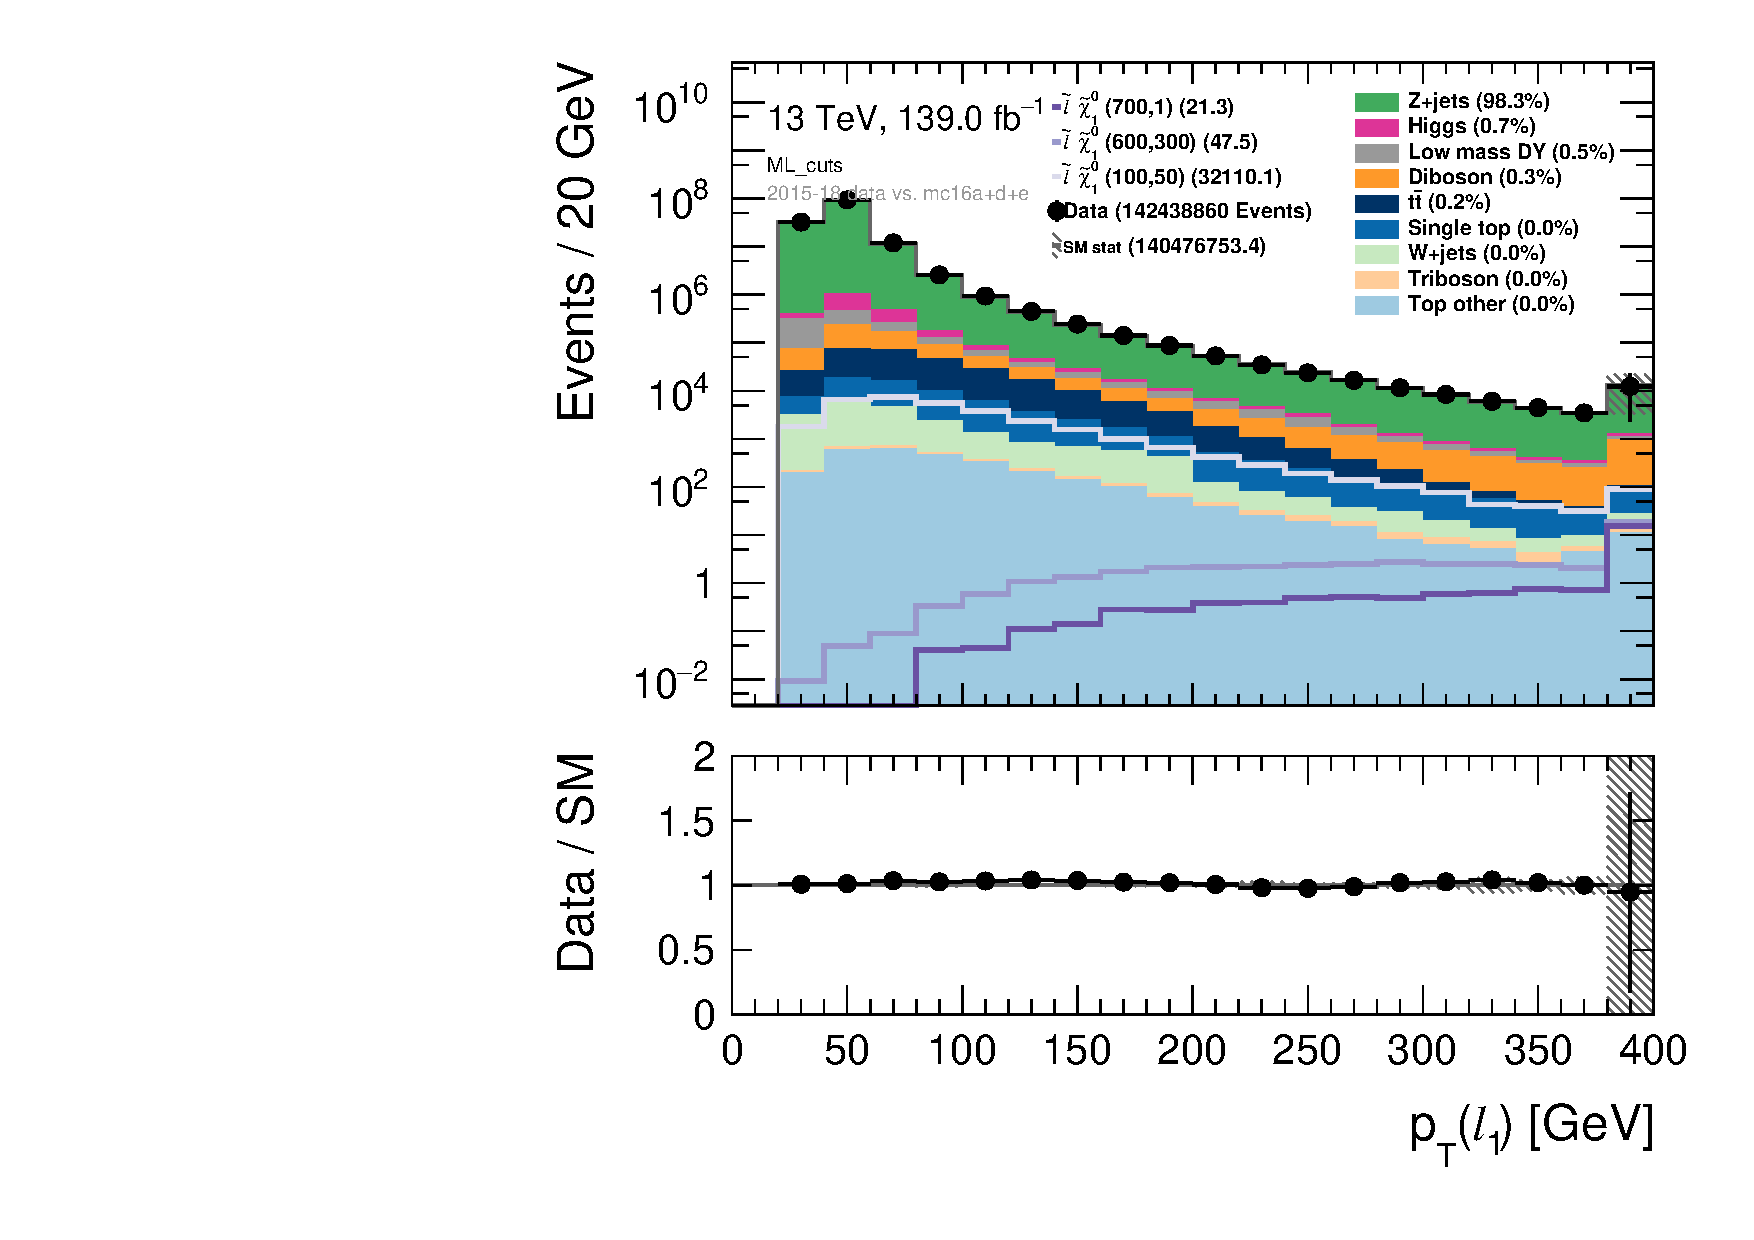
\includegraphics[width=\textwidth]{Figures/SlepSlep/CutAndCount/ML_cuts/hist1d_lepPt[0]_ML_cuts.pdf}
    \caption{The transverse momentum for lepton 1.}
    \label{fig:my_label}
    \end{subfigure}
    \begin{subfigure}[t!]{0.49\textwidth}
        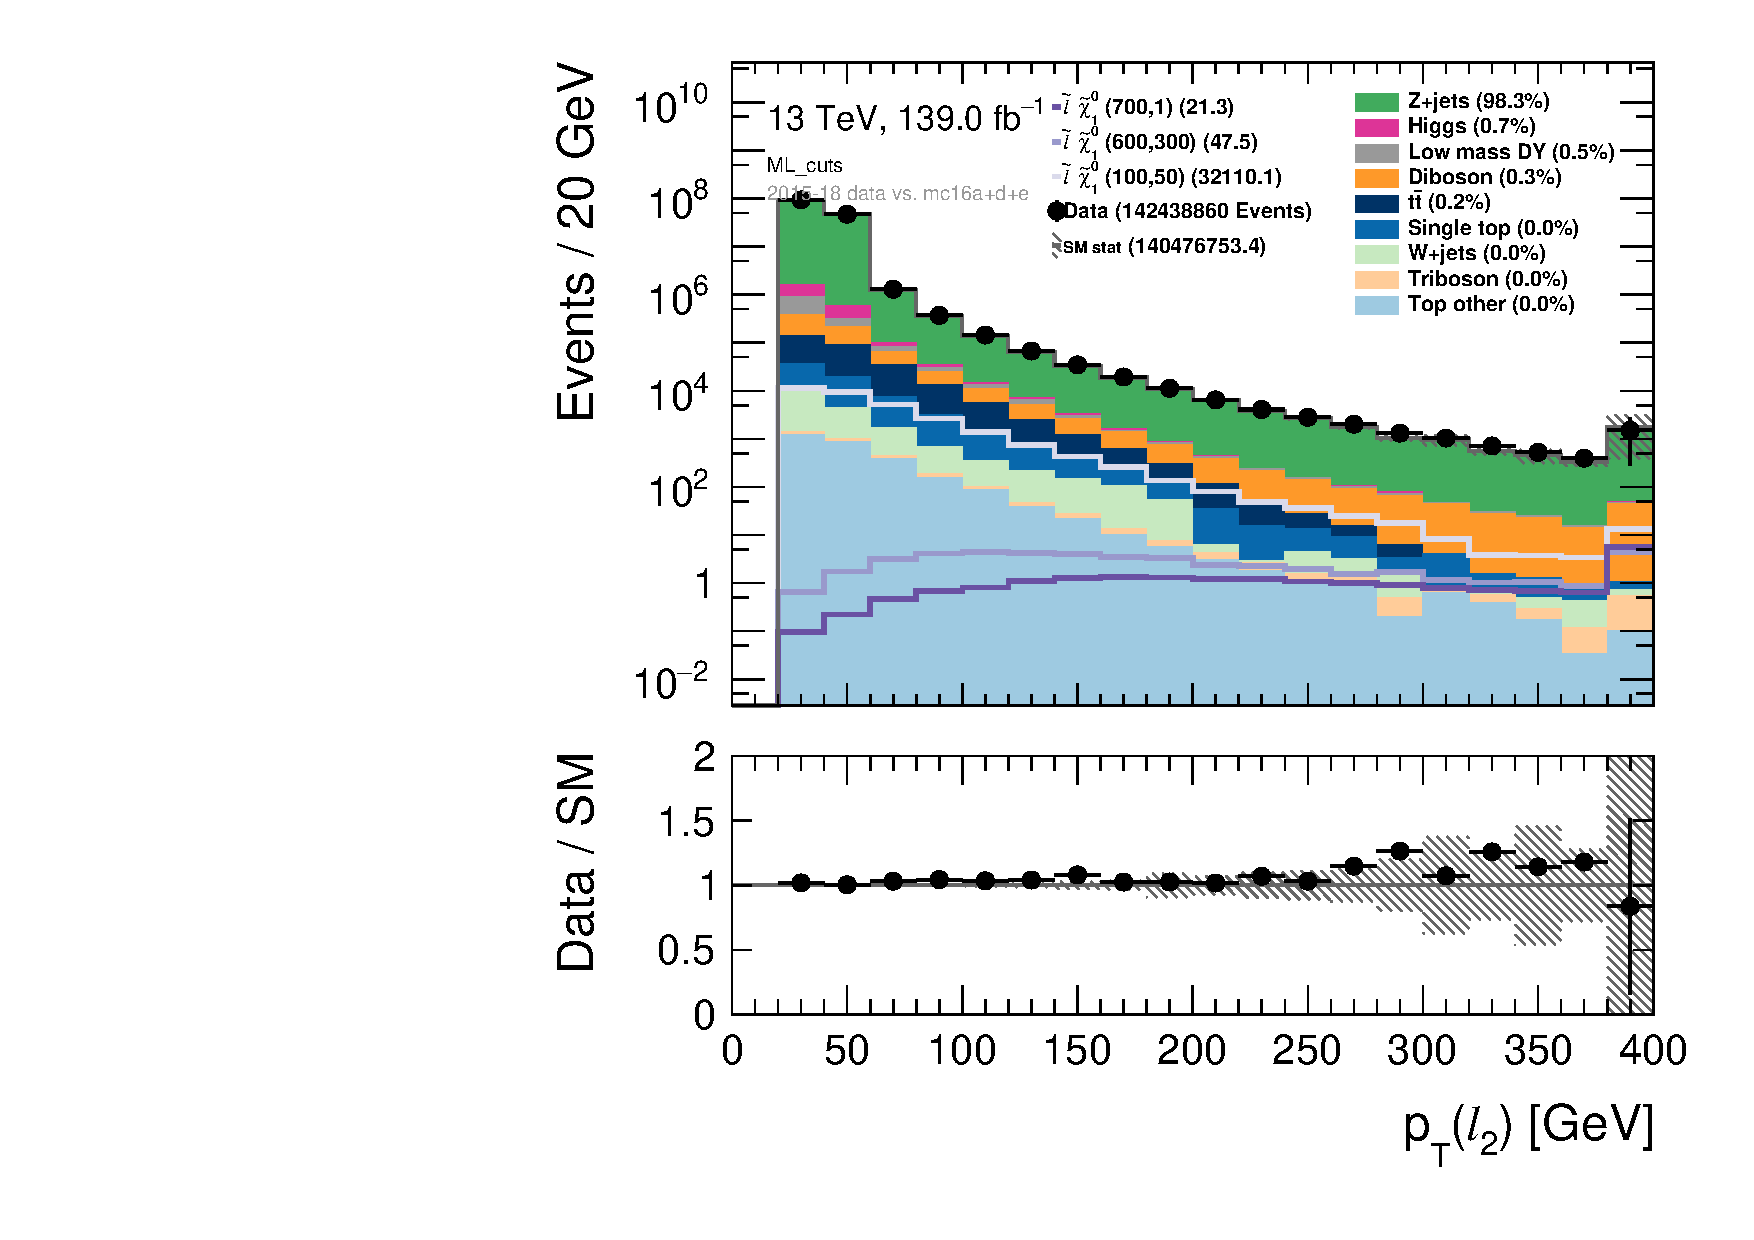
\includegraphics[width=\textwidth]{Figures/SlepSlep/CutAndCount/ML_cuts/hist1d_lepPt[1]_ML_cuts.pdf}
    \caption{Missing transverse energy.}
    \label{fig:my_label}
    \end{subfigure}
    \\
    \begin{subfigure}[t!]{0.49\textwidth}
        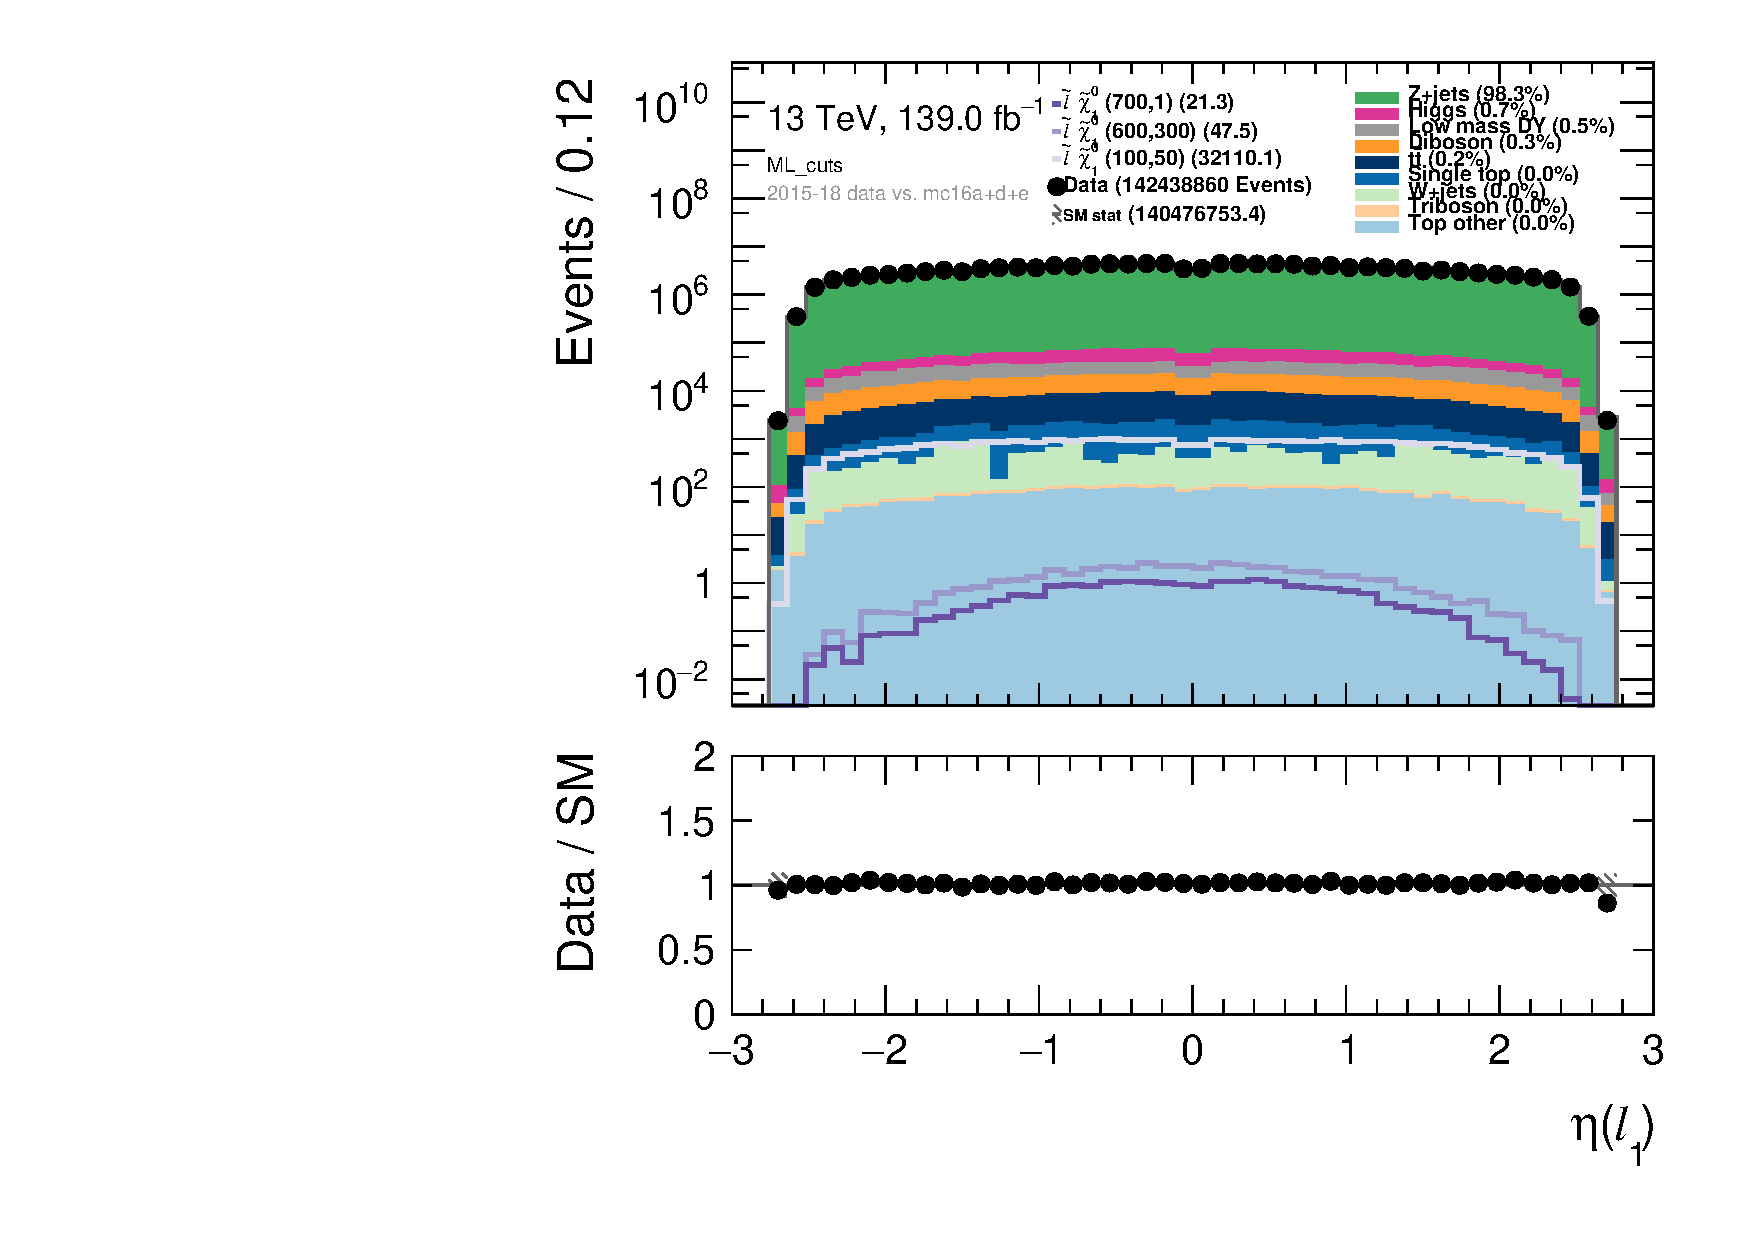
\includegraphics[width=\textwidth]{Figures/SlepSlep/CutAndCount/ML_cuts/hist1d_lepEta[0]_ML_cuts.pdf}
    \caption{The pseudorapidity for lepton 1.}
    \label{fig:my_label}
    \end{subfigure}
    \begin{subfigure}[t!]{0.49\textwidth}
        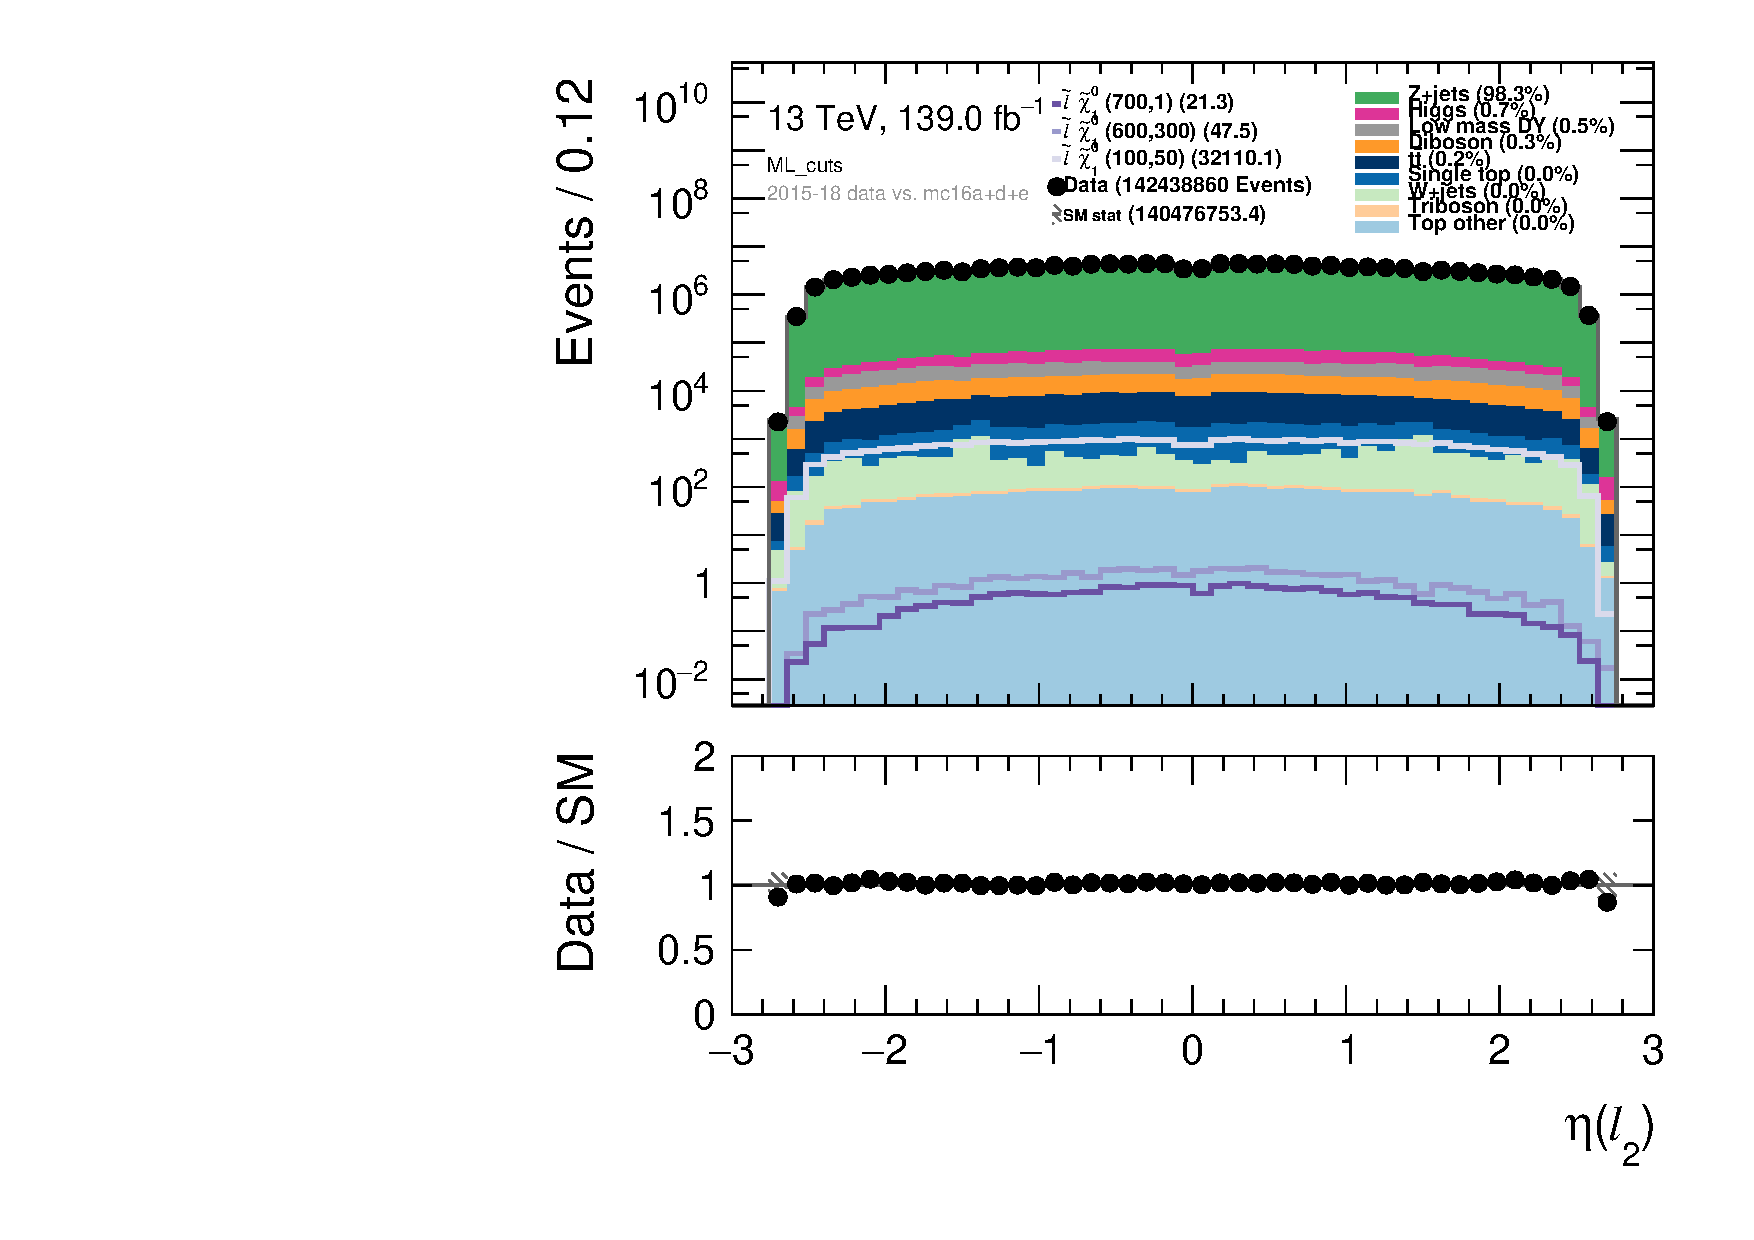
\includegraphics[width=\textwidth]{Figures/SlepSlep/CutAndCount/ML_cuts/hist1d_lepEta[1]_ML_cuts.pdf}
    \caption{The pseudorapidity for lepton 2.}
    \label{fig:my_label}
    \end{subfigure}
    \\
    \begin{subfigure}[t!]{0.49\textwidth}
        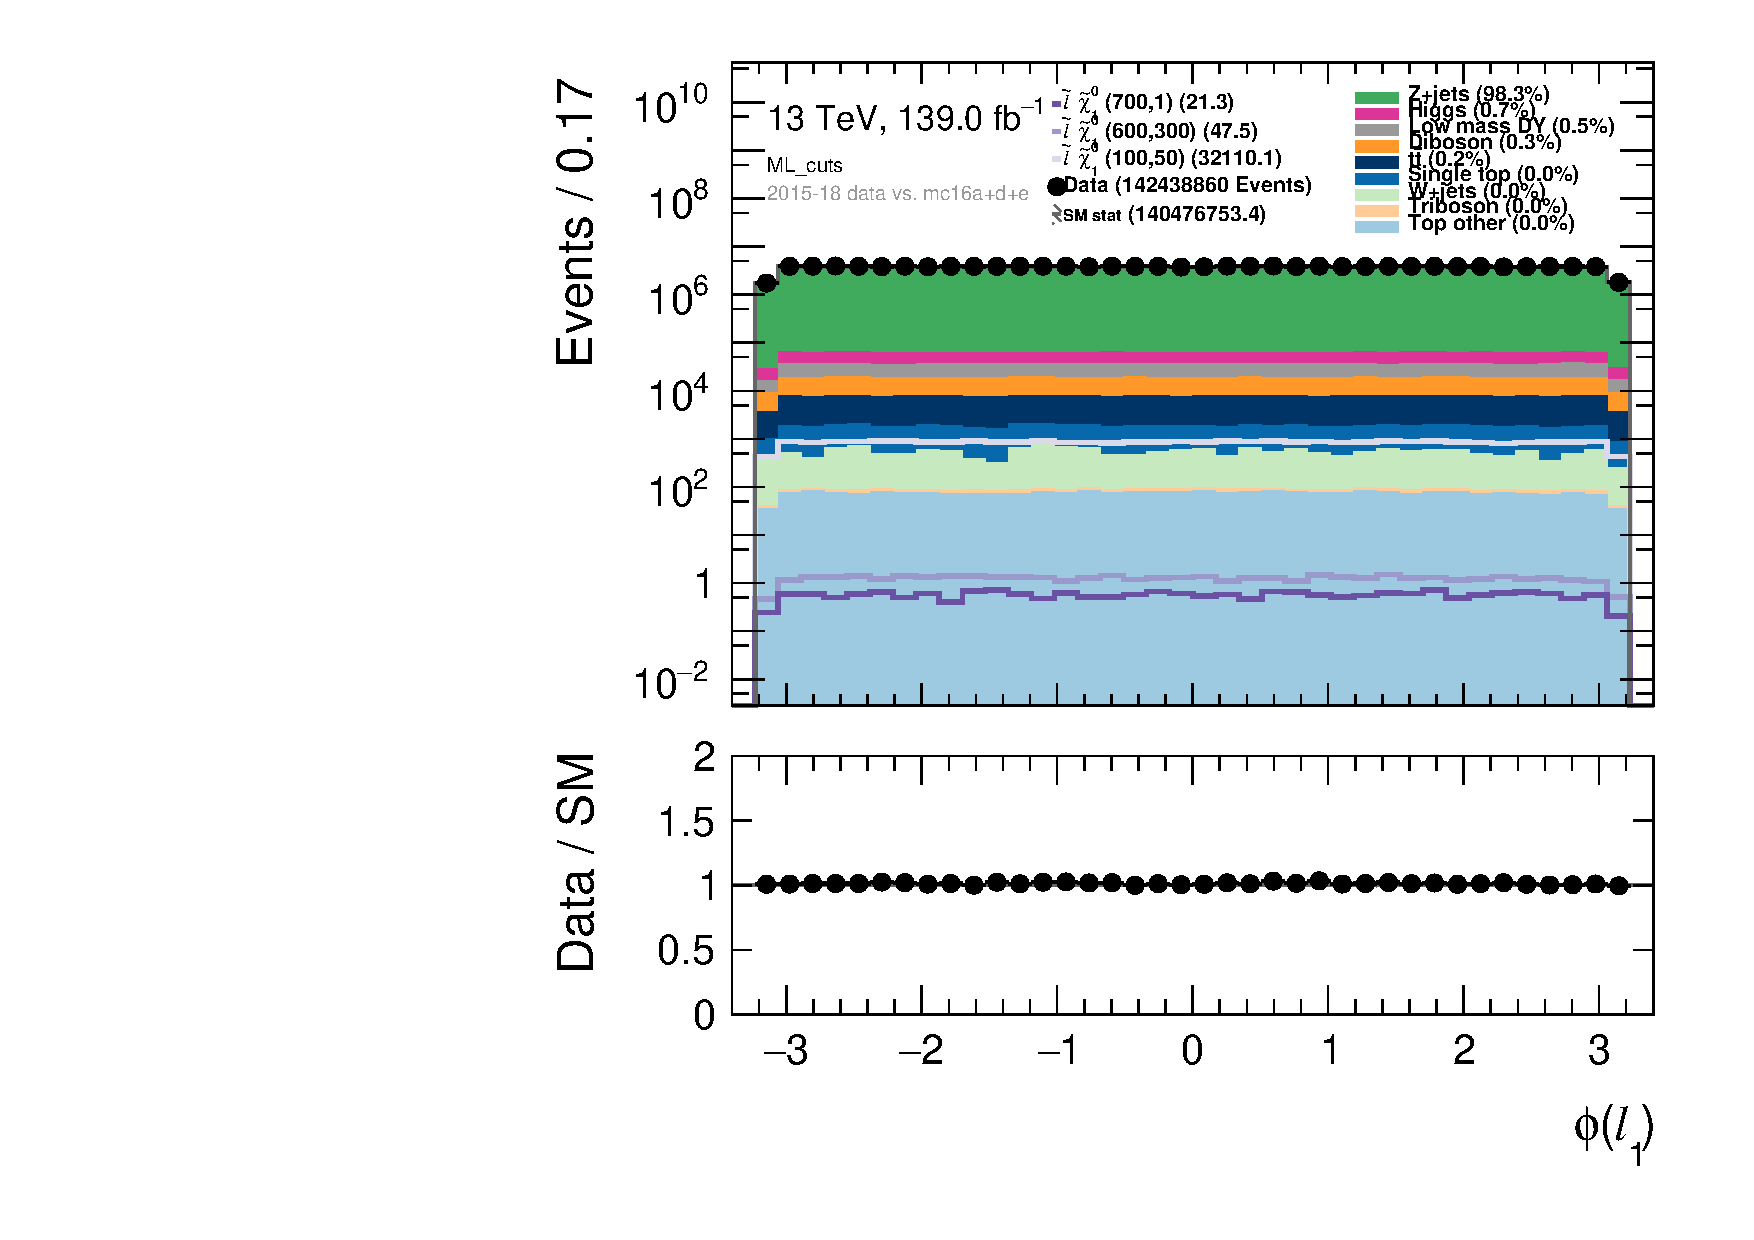
\includegraphics[width=\textwidth]{Figures/SlepSlep/CutAndCount/ML_cuts/hist1d_lepPhi[0]_ML_cuts.pdf}
    \caption{The azimuthal angle for lepton 1.}
    \label{fig:my_label}
    \end{subfigure}
    \begin{subfigure}[t!]{0.49\textwidth}
        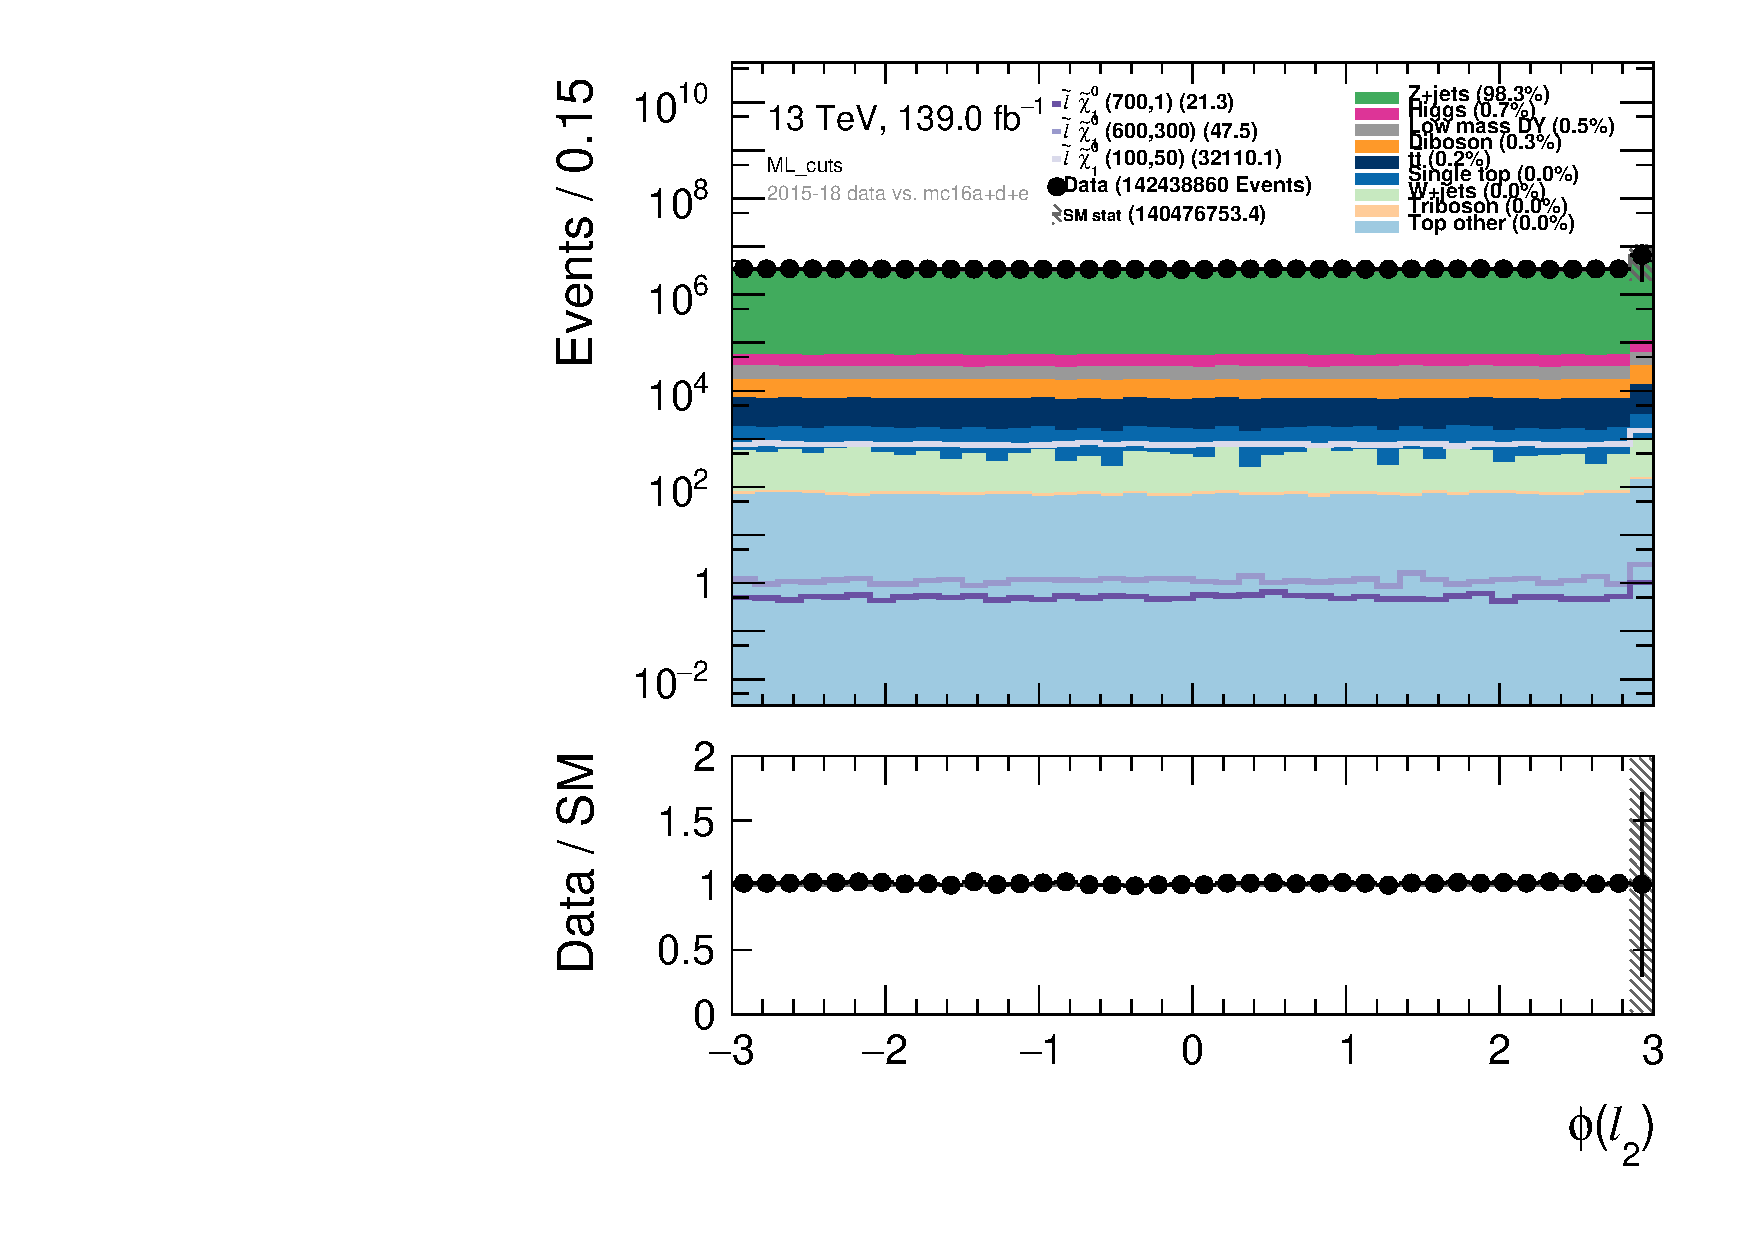
\includegraphics[width=\textwidth]{Figures/SlepSlep/CutAndCount/ML_cuts/hist1d_lepPhi[1]_ML_cuts.pdf}
    \caption{The azimuthal angle for lepton 2.}
    \label{fig:my_label}
    \end{subfigure}
\end{figure}

\begin{figure}[H]\ContinuedFloat
%\begin{minipage}{2\textwidth}
%\begin{adjustwidth}{-3cm}{-3cm}
\centering
    \begin{subfigure}[t!]{0.49\textwidth}
        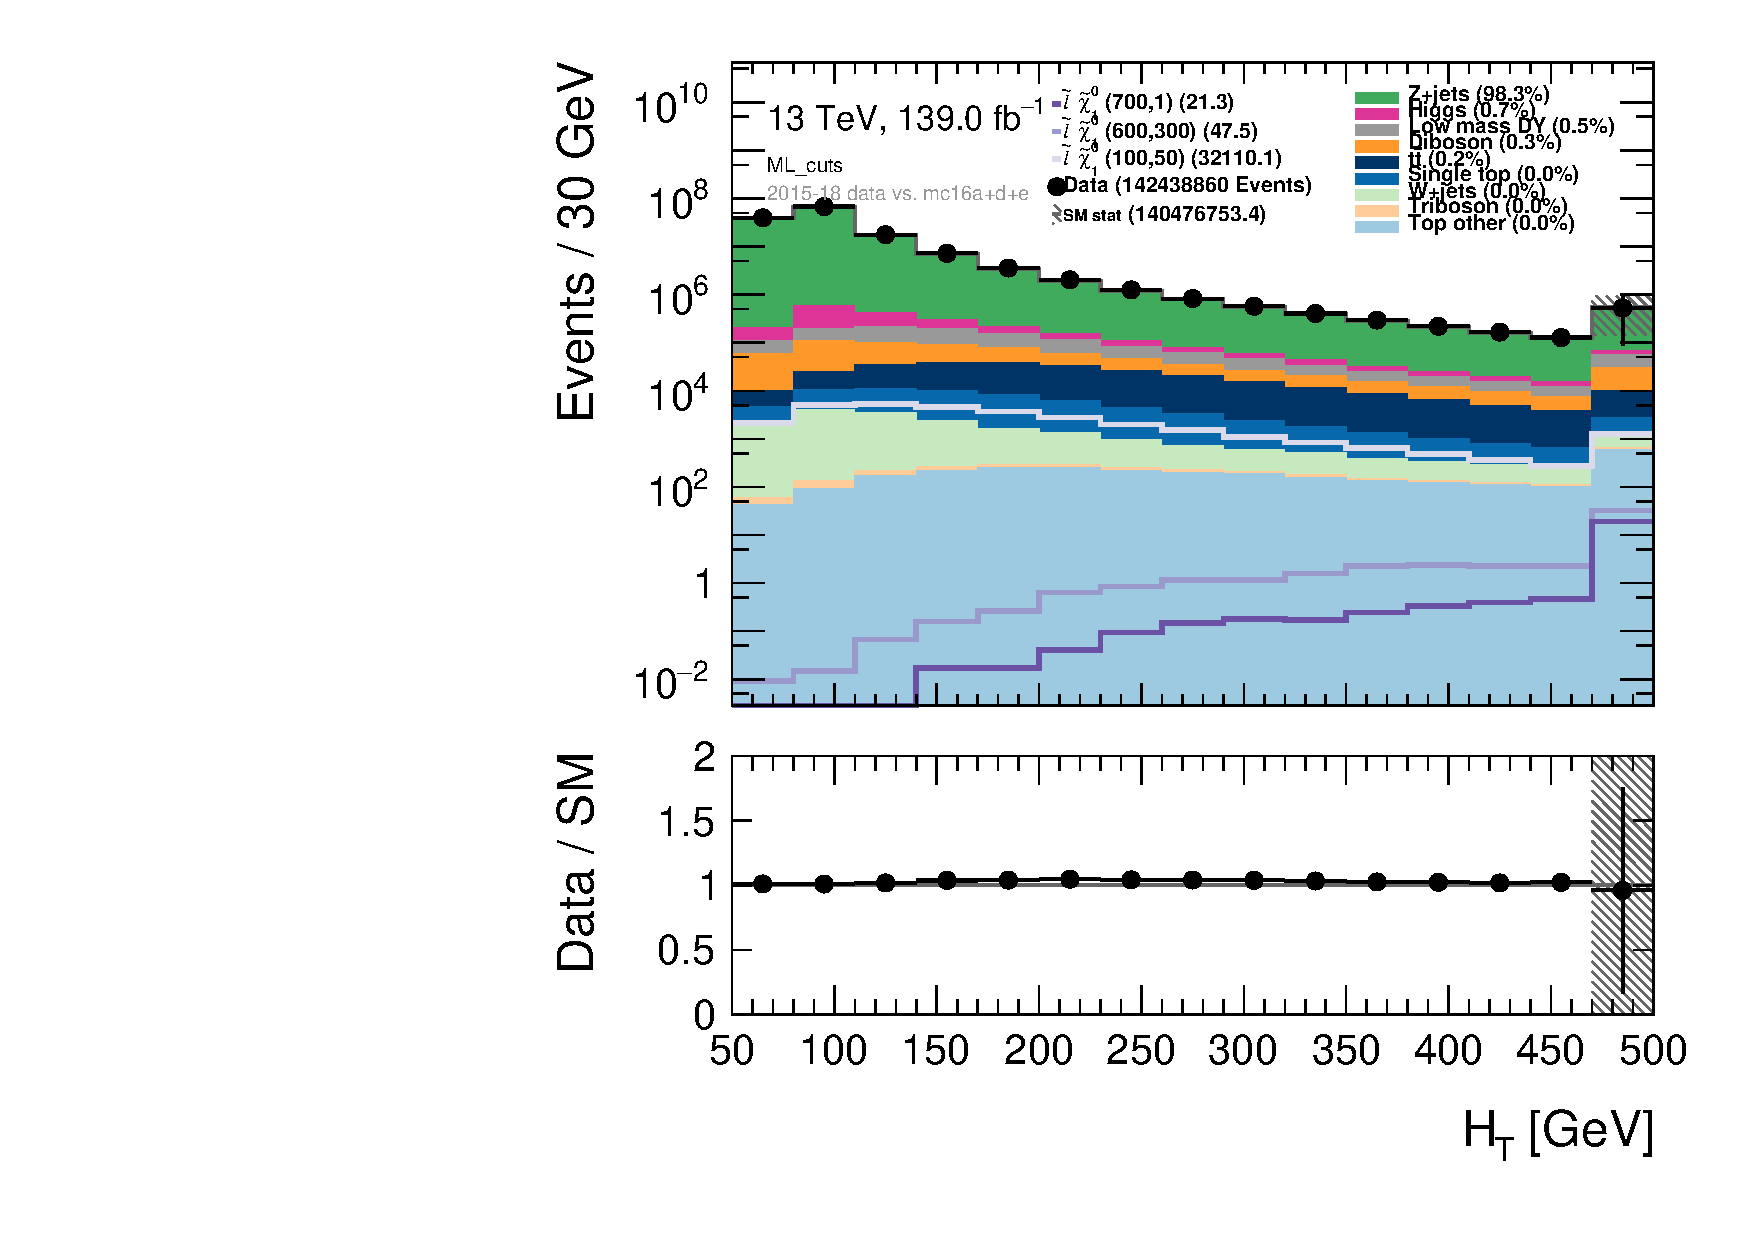
\includegraphics[width=\textwidth]{Figures/SlepSlep/CutAndCount/ML_cuts/hist1d_HT_ML_cuts.pdf}
    \caption{The scalar sum of the $p_T$ of the selected jets and leptons.}
    \label{fig:my_label}
    \end{subfigure}
    \begin{subfigure}[t!]{0.49\textwidth}
        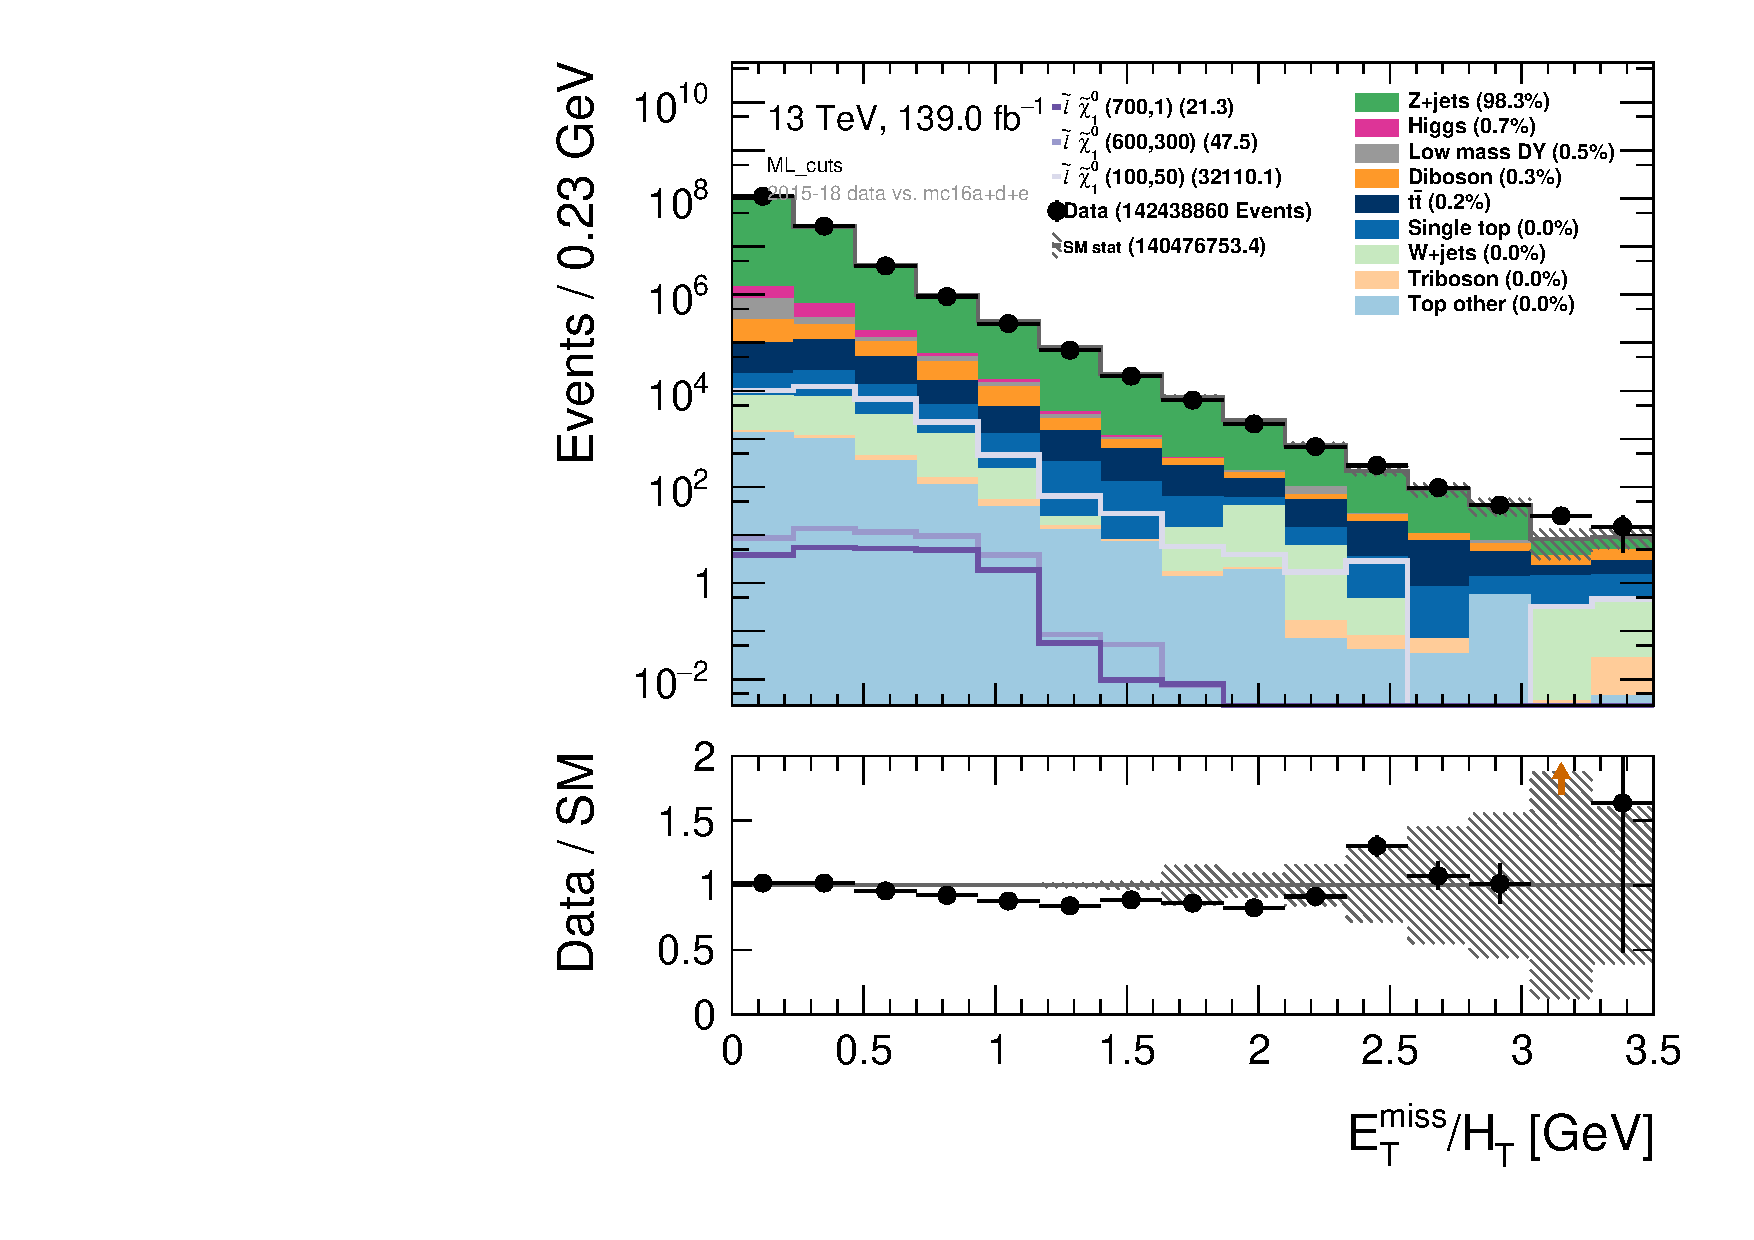
\includegraphics[width=\textwidth]{Figures/SlepSlep/CutAndCount/ML_cuts/hist1d_met_HT_ML_cuts.pdf}
    \caption{The ratio between $E_T^{miss}$ and $H_T$.}
    \label{fig:my_label}
    \end{subfigure}
    \begin{subfigure}[t!]{0.49\textwidth}
        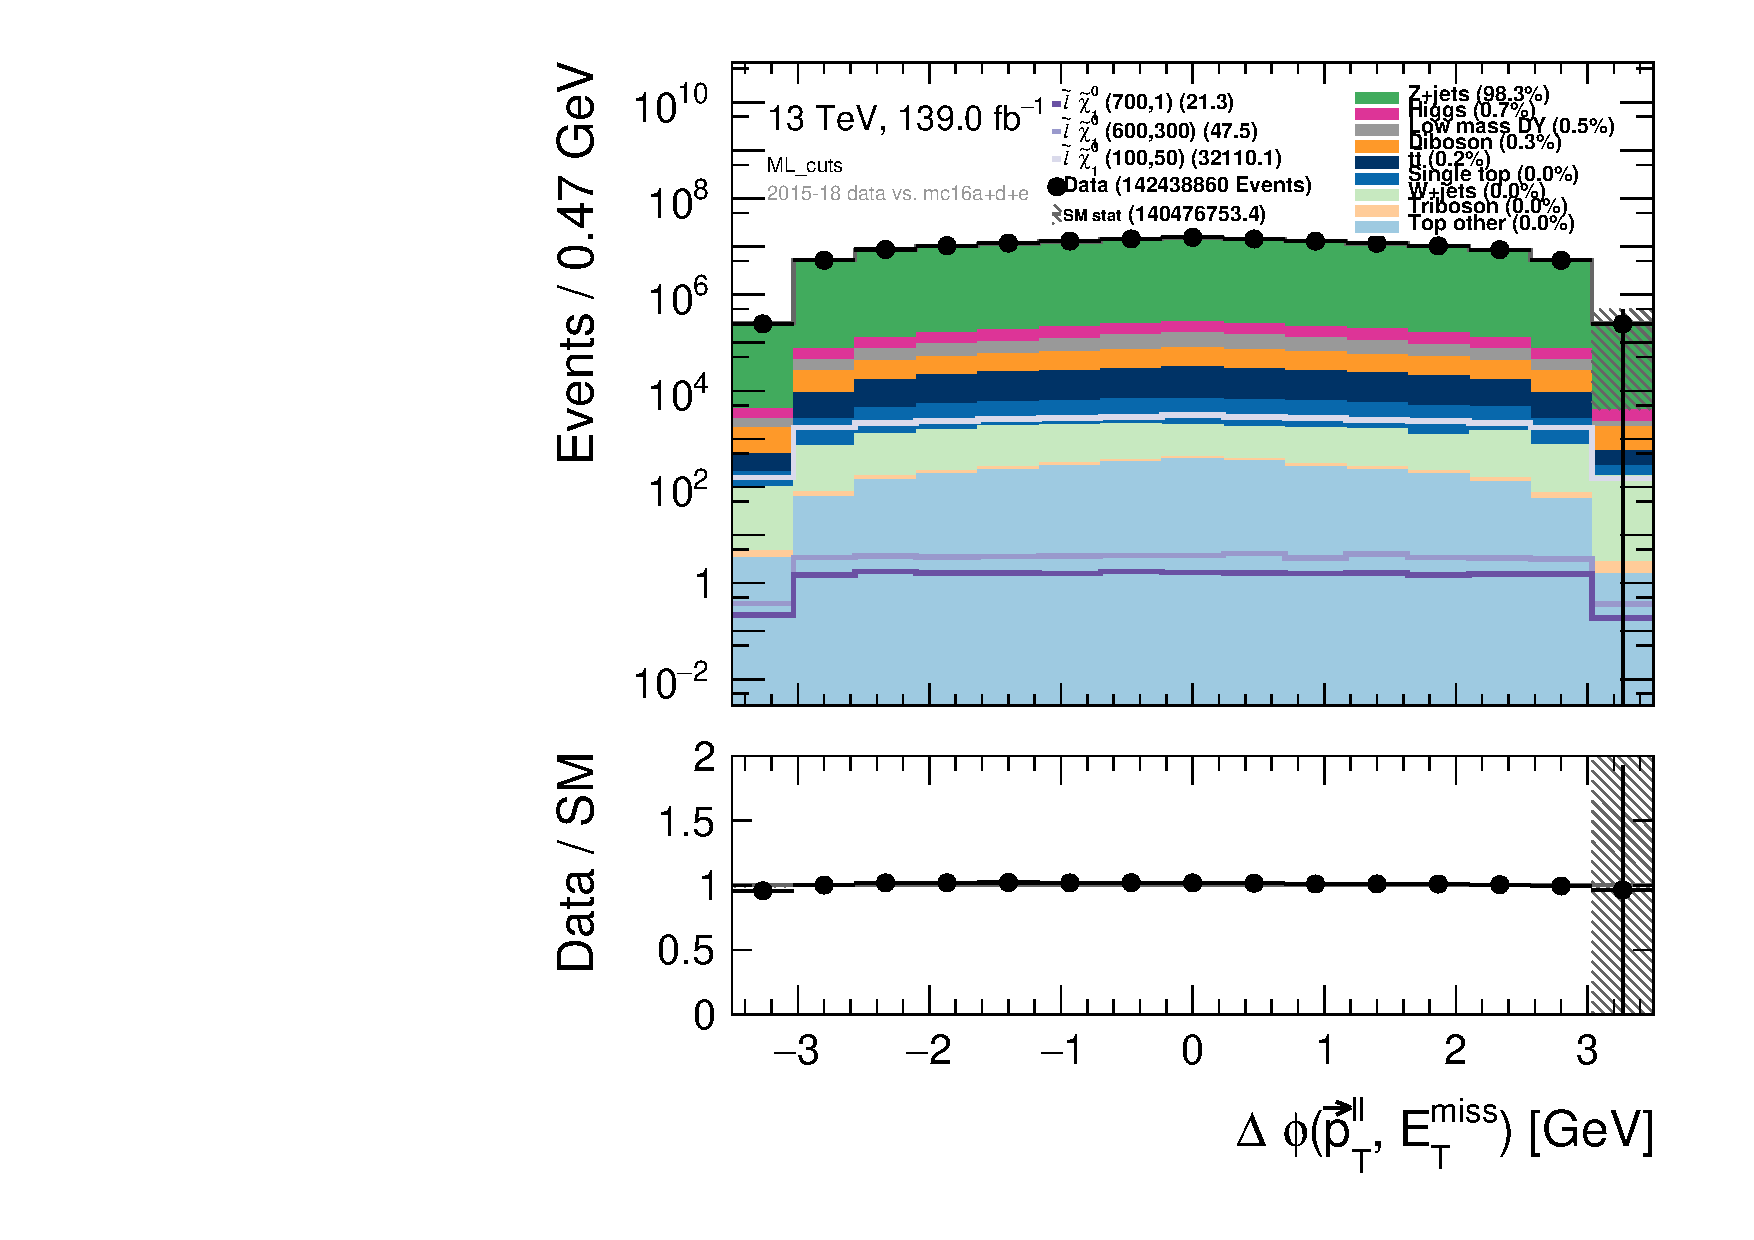
\includegraphics[width=\textwidth]{Figures/SlepSlep/CutAndCount/ML_cuts/hist1d_deltaPhi_ML_cuts.pdf}
    \caption{The azimuthal angle difference between the dilepton system and $E_T^{miss}$.}
    \label{fig:my_label}
    \end{subfigure}
    \begin{subfigure}[t!]{0.49\textwidth}
        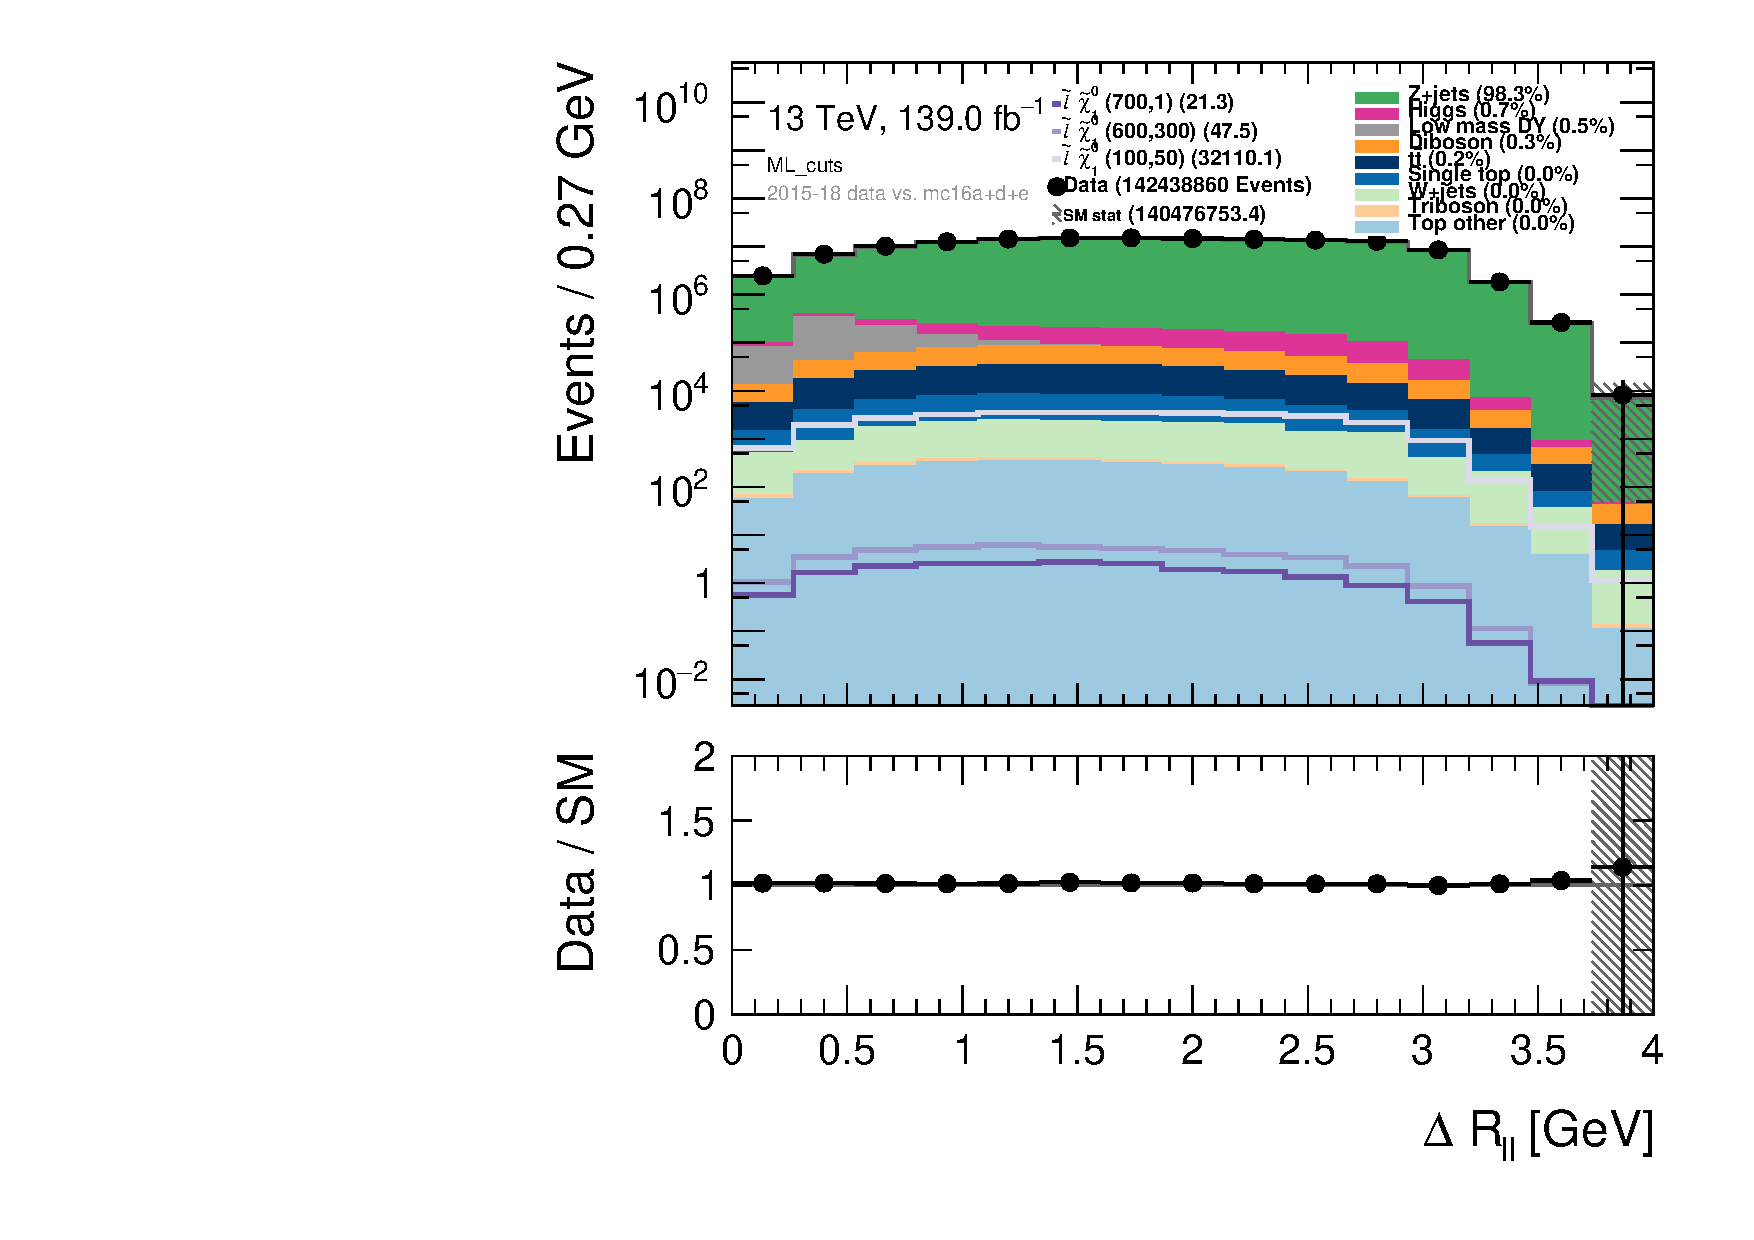
\includegraphics[width=\textwidth]{Figures/SlepSlep/CutAndCount/ML_cuts/hist1d_deltaRll_ML_cuts.pdf}
    \caption{Distance between the two leptons.}
    \label{fig:my_label}
    \end{subfigure}
    \begin{subfigure}[t!]{0.49\textwidth}
        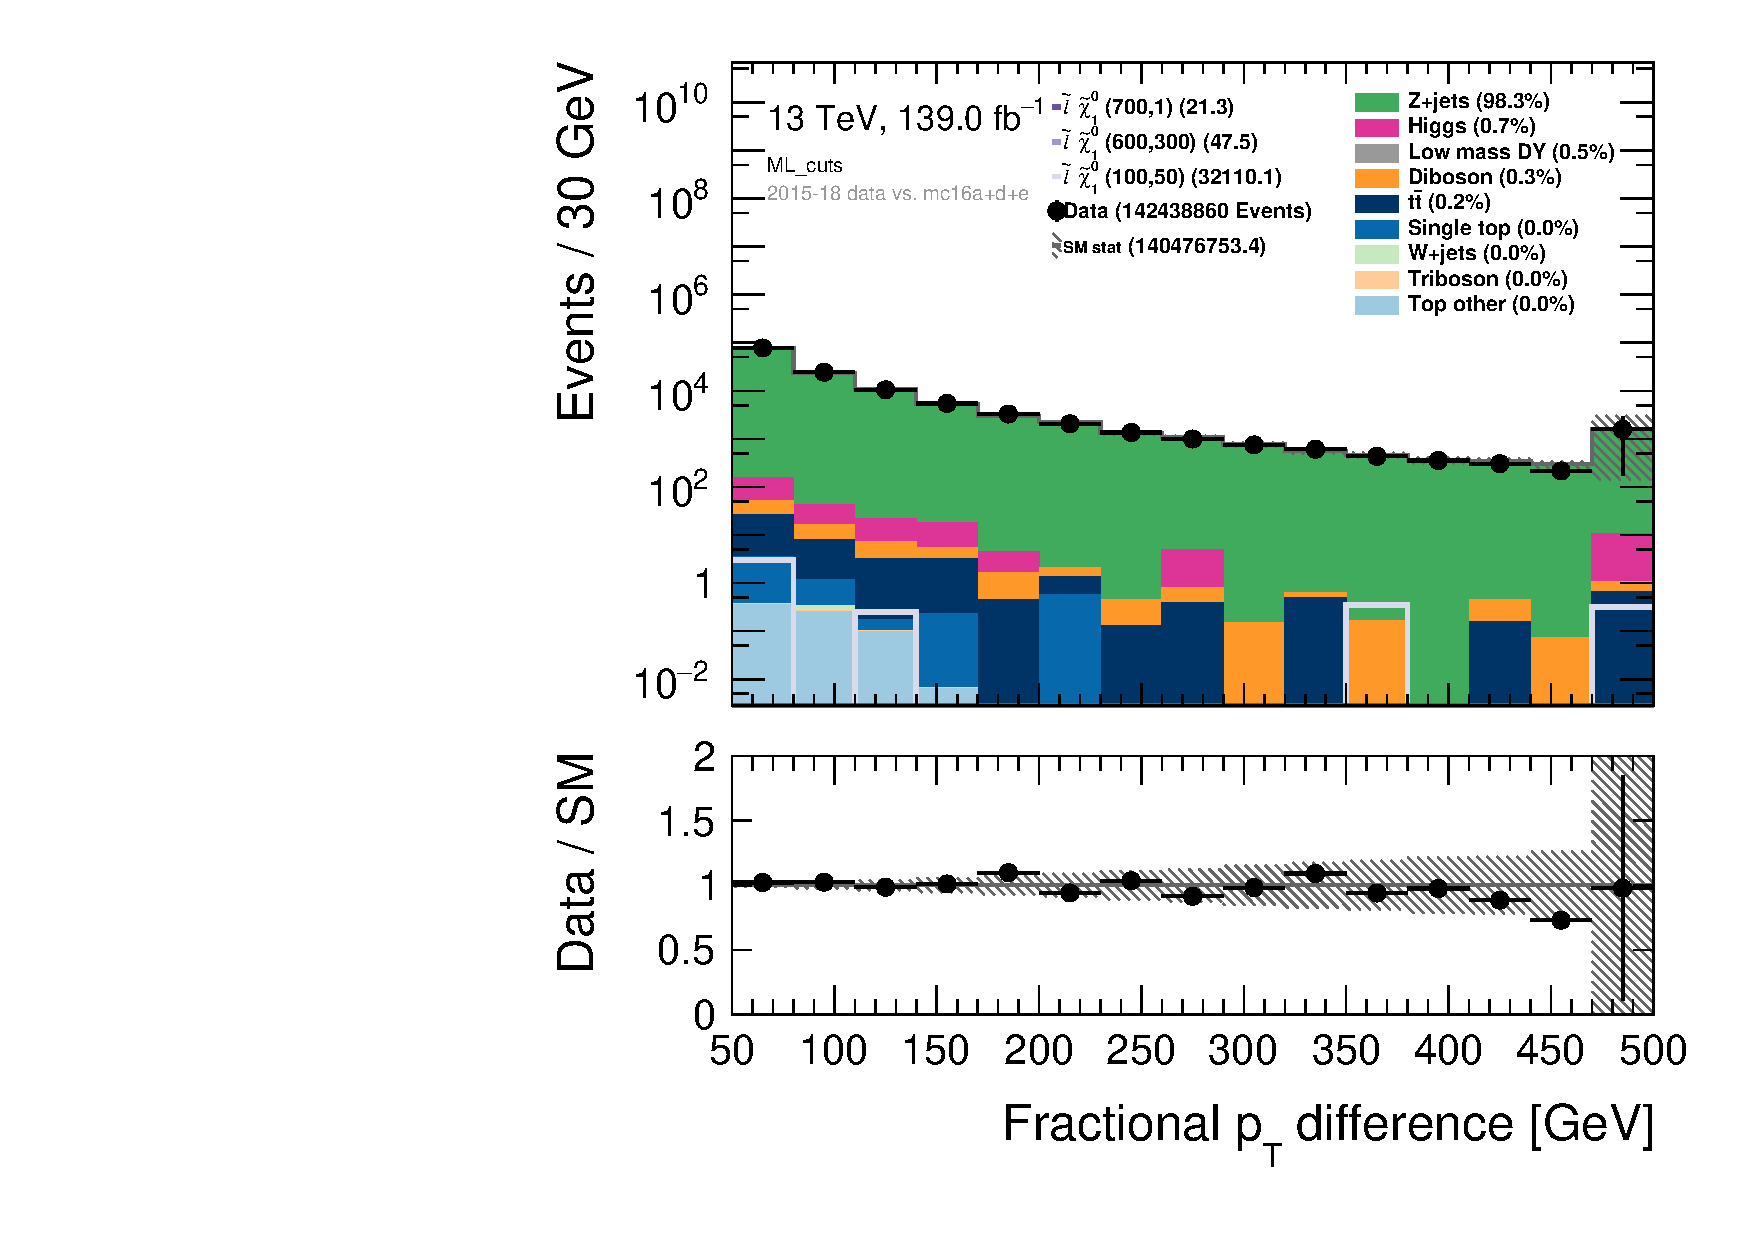
\includegraphics[width=\textwidth]{Figures/SlepSlep/CutAndCount/ML_cuts/hist1d_pTdiff_ML_cuts.pdf}
    \caption{The difference between the dilepton $p_T$, the selected jets $p_T$ and the vector sum of $\Vec{E}_T^{miss}$.}
    \label{fig:my_label}
    \end{subfigure}
    \begin{subfigure}[t!]{0.49\textwidth}
        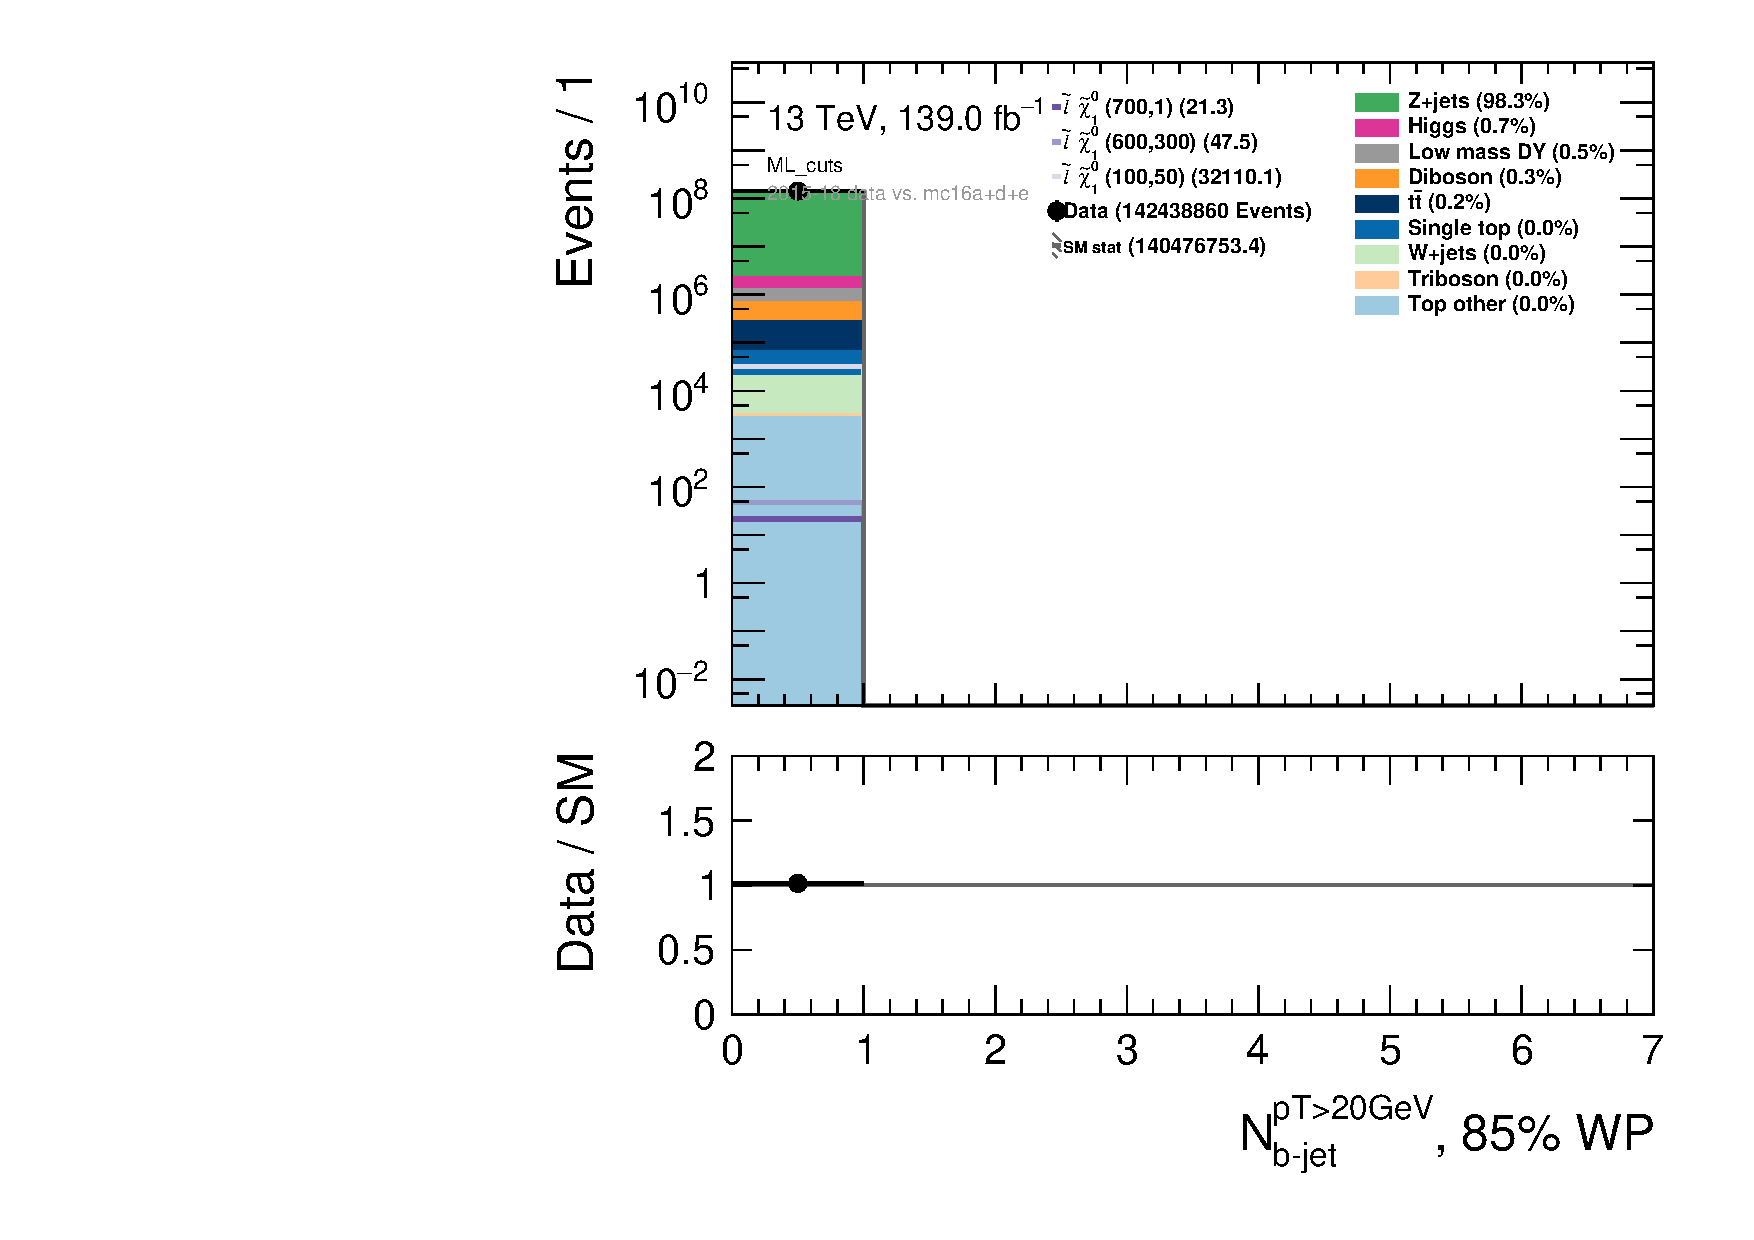
\includegraphics[width=\textwidth]{Figures/SlepSlep/CutAndCount/ML_cuts/hist1d_nBJet20_MV2c10_FixedCutBEff_85_ML_cuts.pdf}
    \caption{B-jets.}
    \label{fig:my_label}
    \end{subfigure}
\end{figure}

\begin{figure}[H]\ContinuedFloat
%\begin{minipage}{2\textwidth}
%\begin{adjustwidth}{-3cm}{-3cm}
\centering
%\advance\leftskip-4cm 
%\advance\rightskip-4cm 
    \begin{subfigure}[t!]{0.49\textwidth}
        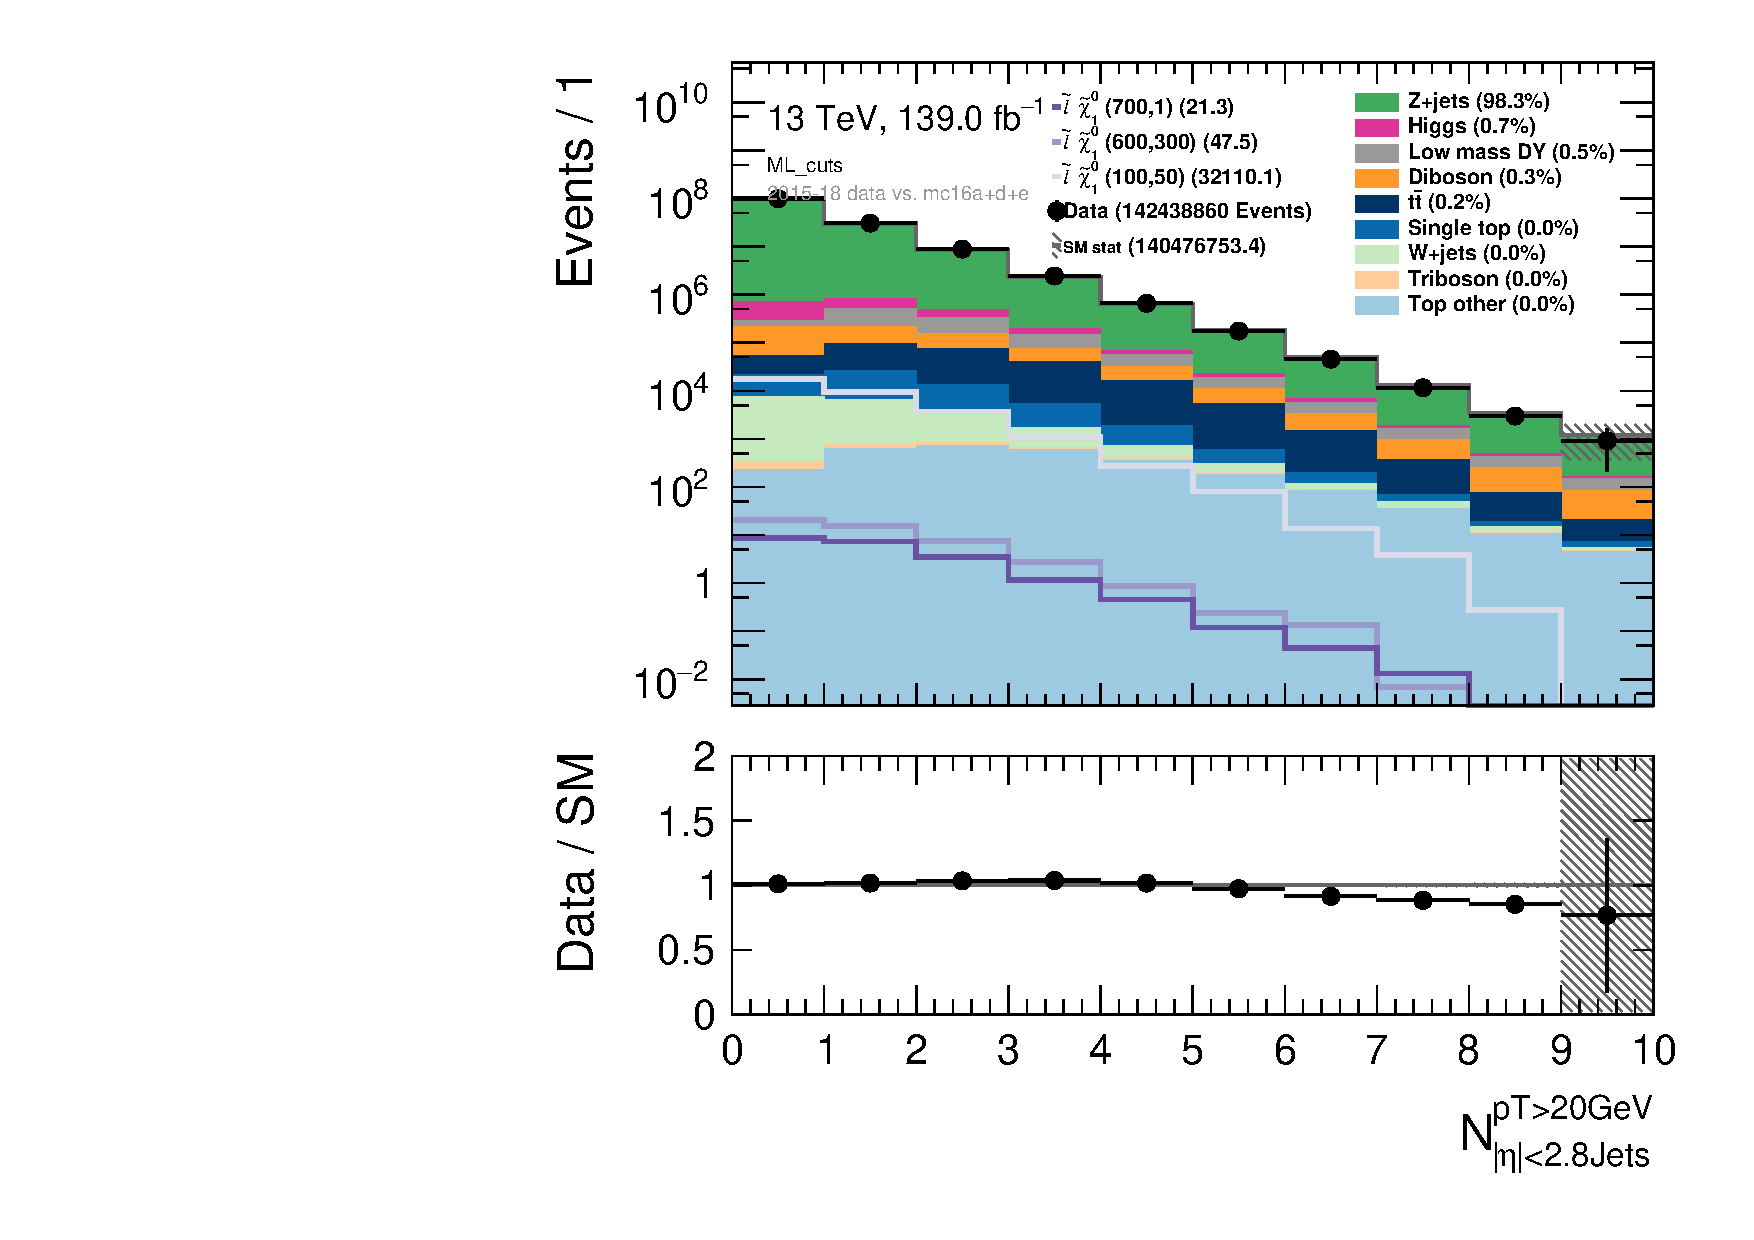
\includegraphics[width=\textwidth]{Figures/SlepSlep/CutAndCount/ML_cuts/hist1d_nJet20_ML_cuts.pdf}
    \caption{Jets with $p_T > 20$ GeV.}
    \label{fig:my_label}
    \end{subfigure}
    \begin{subfigure}[t!]{0.49\textwidth}
        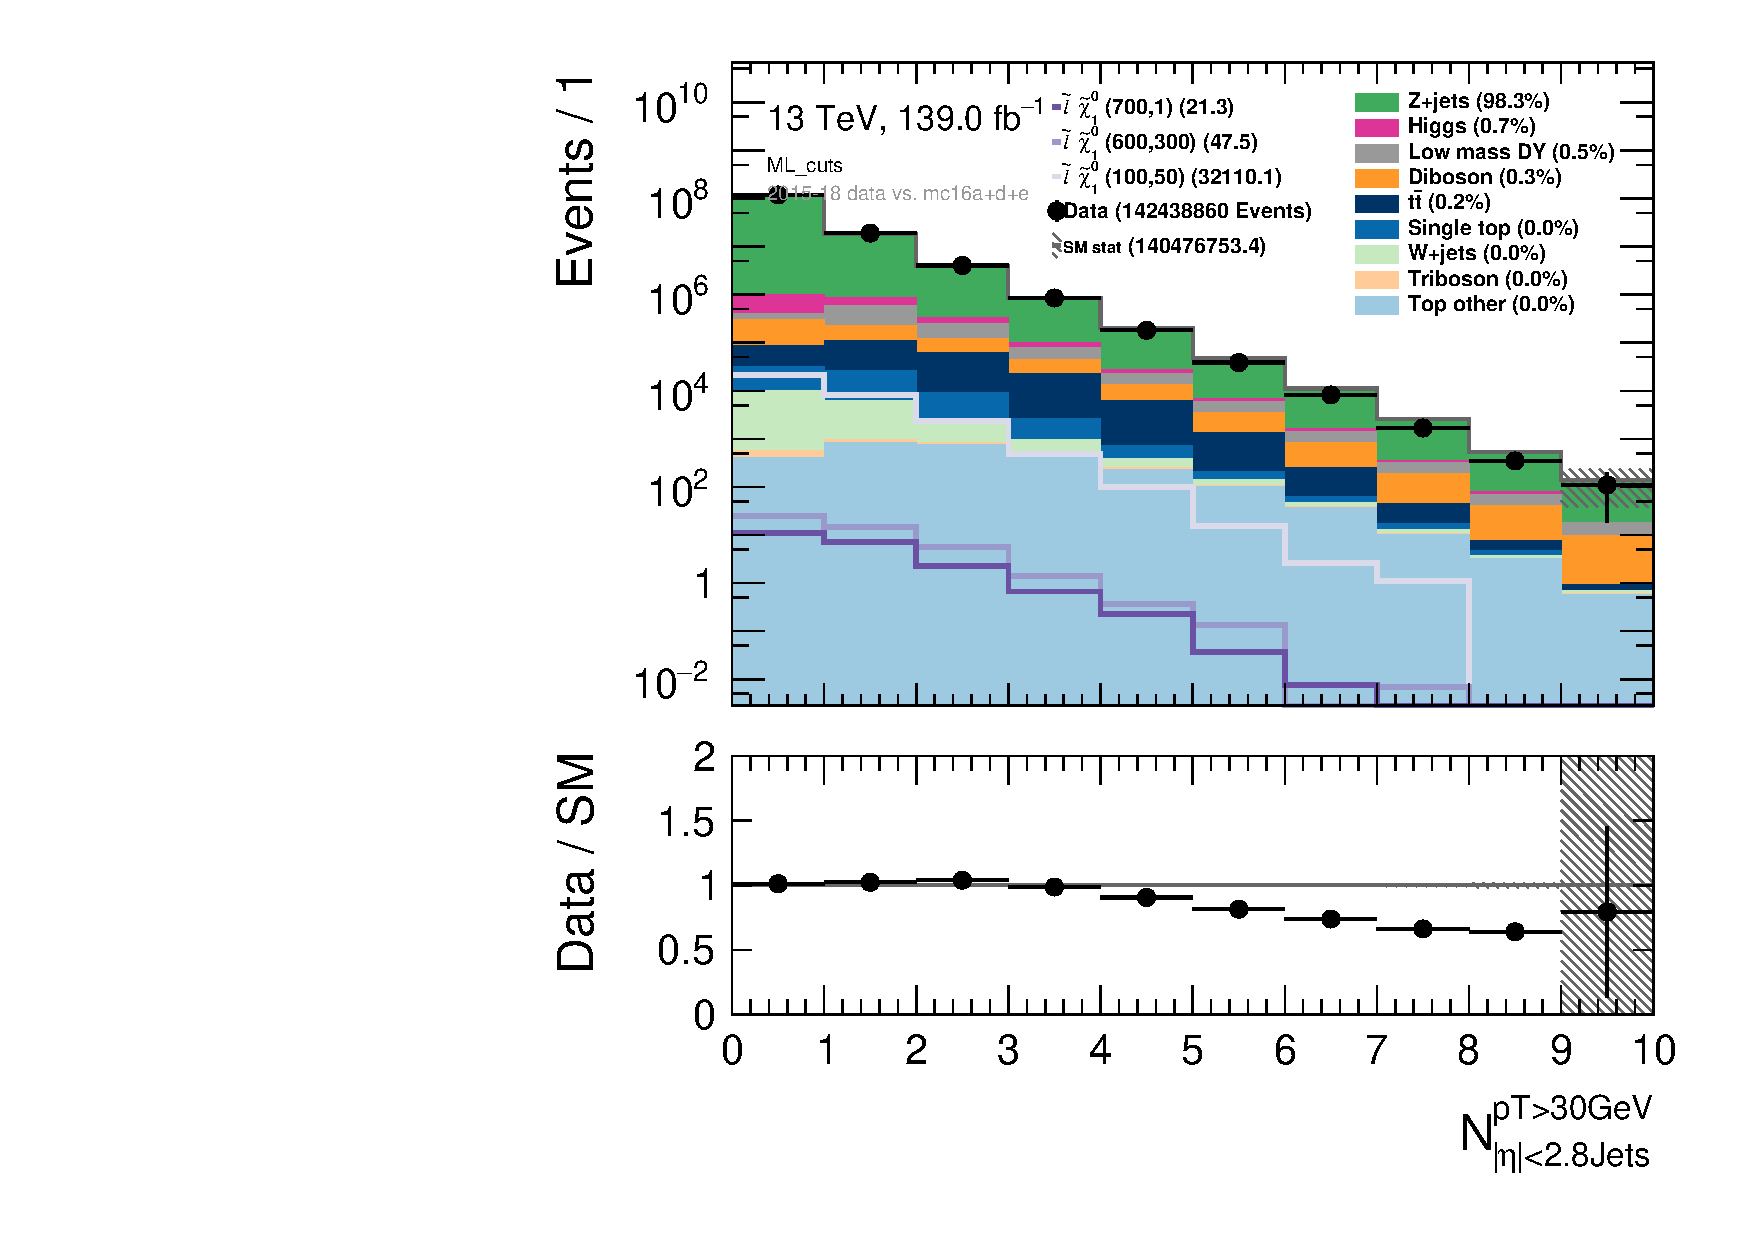
\includegraphics[width=\textwidth]{Figures/SlepSlep/CutAndCount/ML_cuts/hist1d_nJet30_ML_cuts.pdf}
   \caption{Jets with $p_T > 30$ GeV.}
   \label{fig:my_label}
    \end{subfigure}
    \\
    \begin{subfigure}[t!]{0.49\textwidth}
        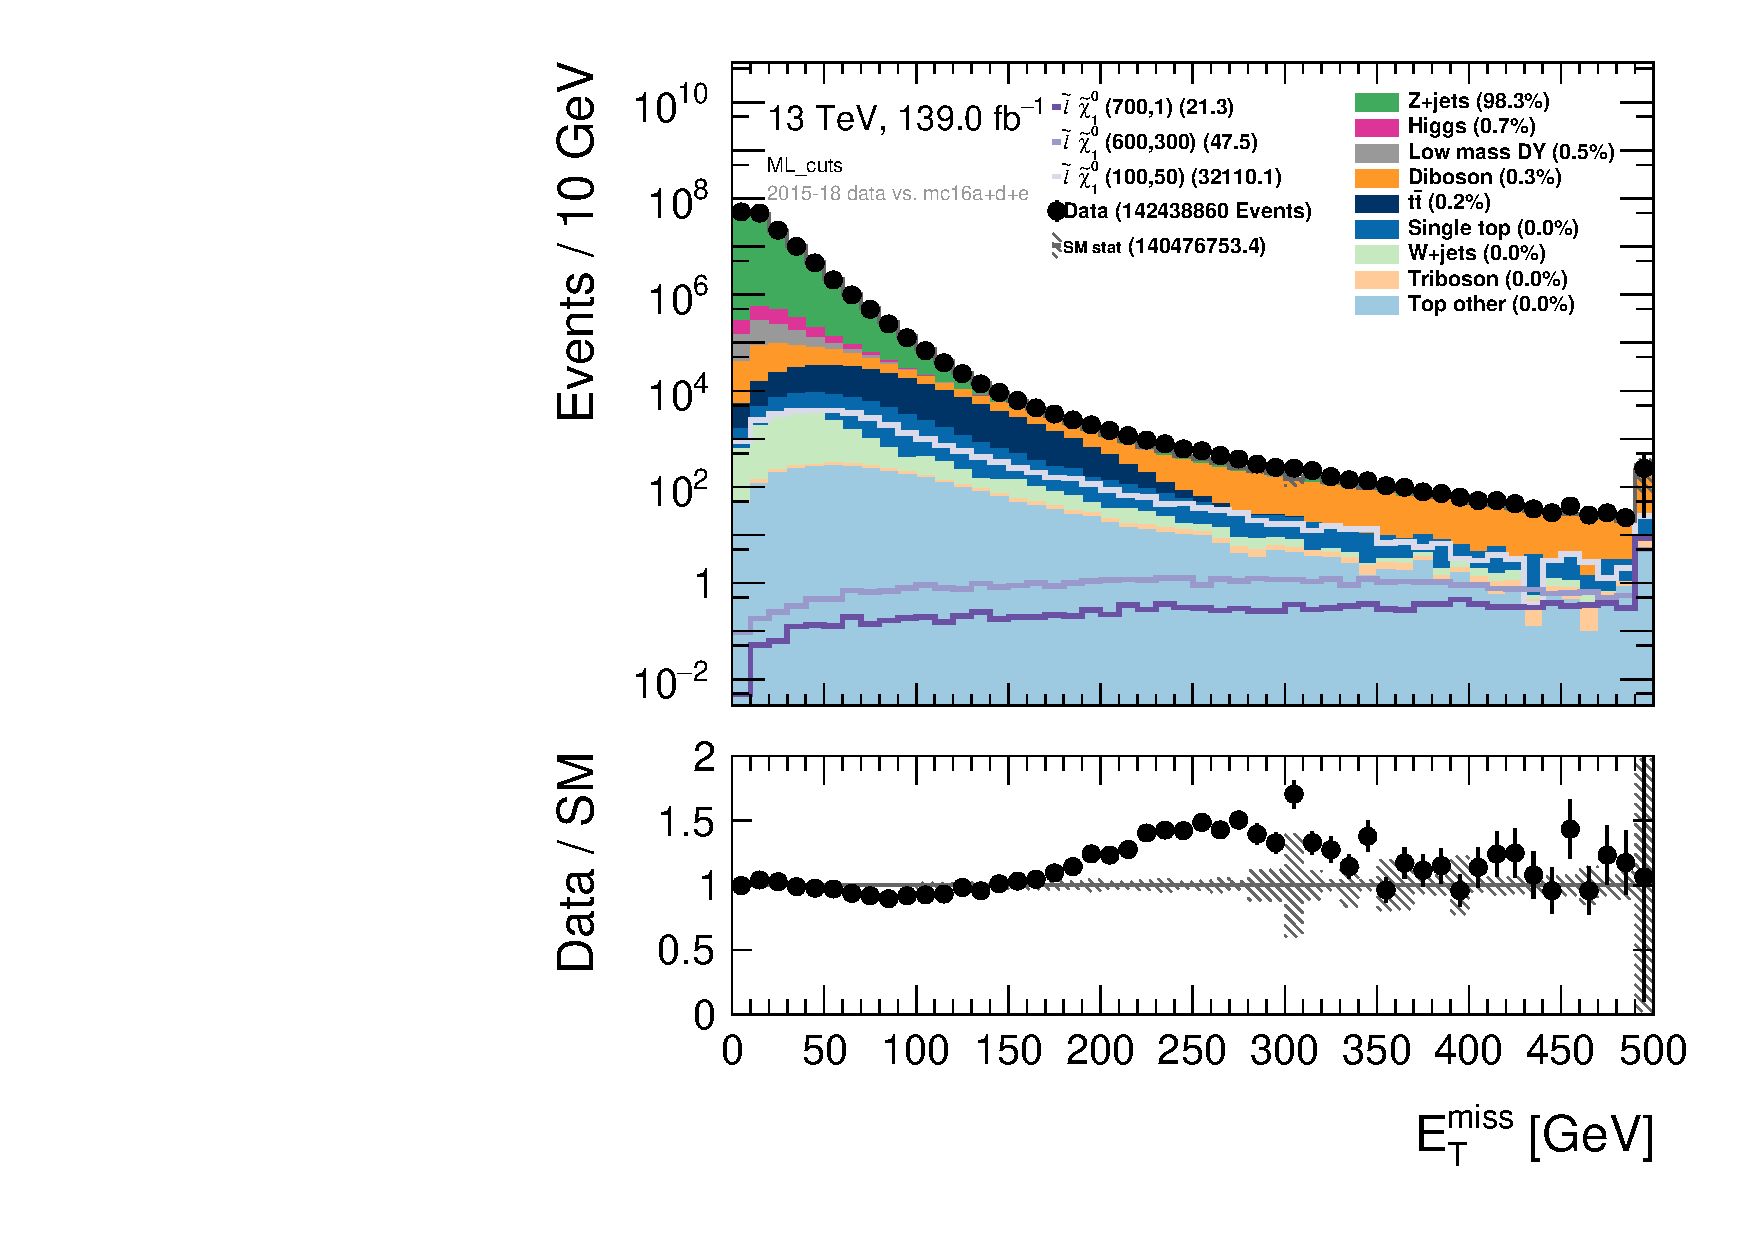
\includegraphics[width=\textwidth]{Figures/SlepSlep/CutAndCount/ML_cuts/hist1d_met_Et_ML_cuts.pdf}
    \caption{Missing transverse energy.}
    \label{fig:my_label}
    \end{subfigure}
    \begin{subfigure}[t!]{0.49\textwidth}
        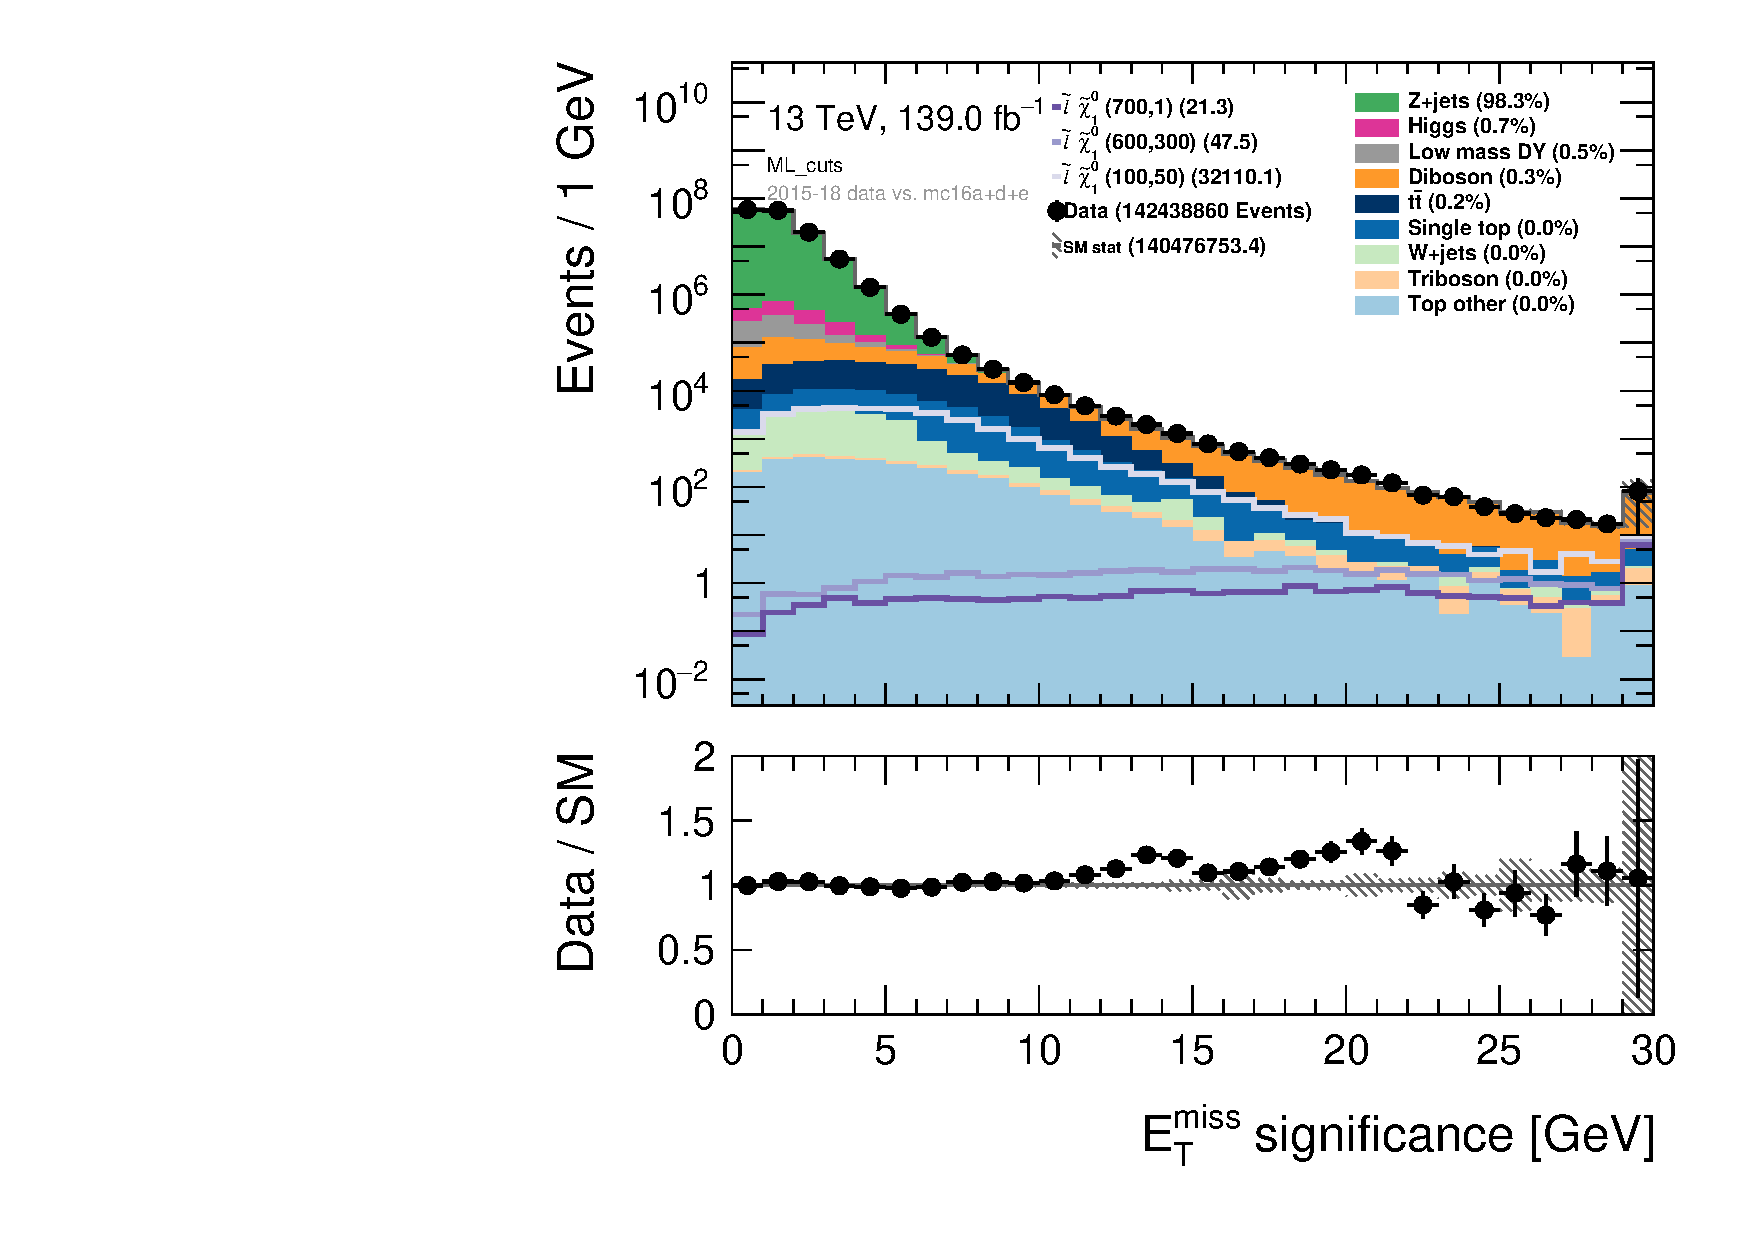
\includegraphics[width=\textwidth]{Figures/SlepSlep/CutAndCount/ML_cuts/hist1d_met_Sign_ML_cuts.pdf}
    \caption{Missing transverse energy significance.}
    \label{fig:my_label}
    \end{subfigure}
    \\
    \begin{subfigure}[t!]{0.49\textwidth}
        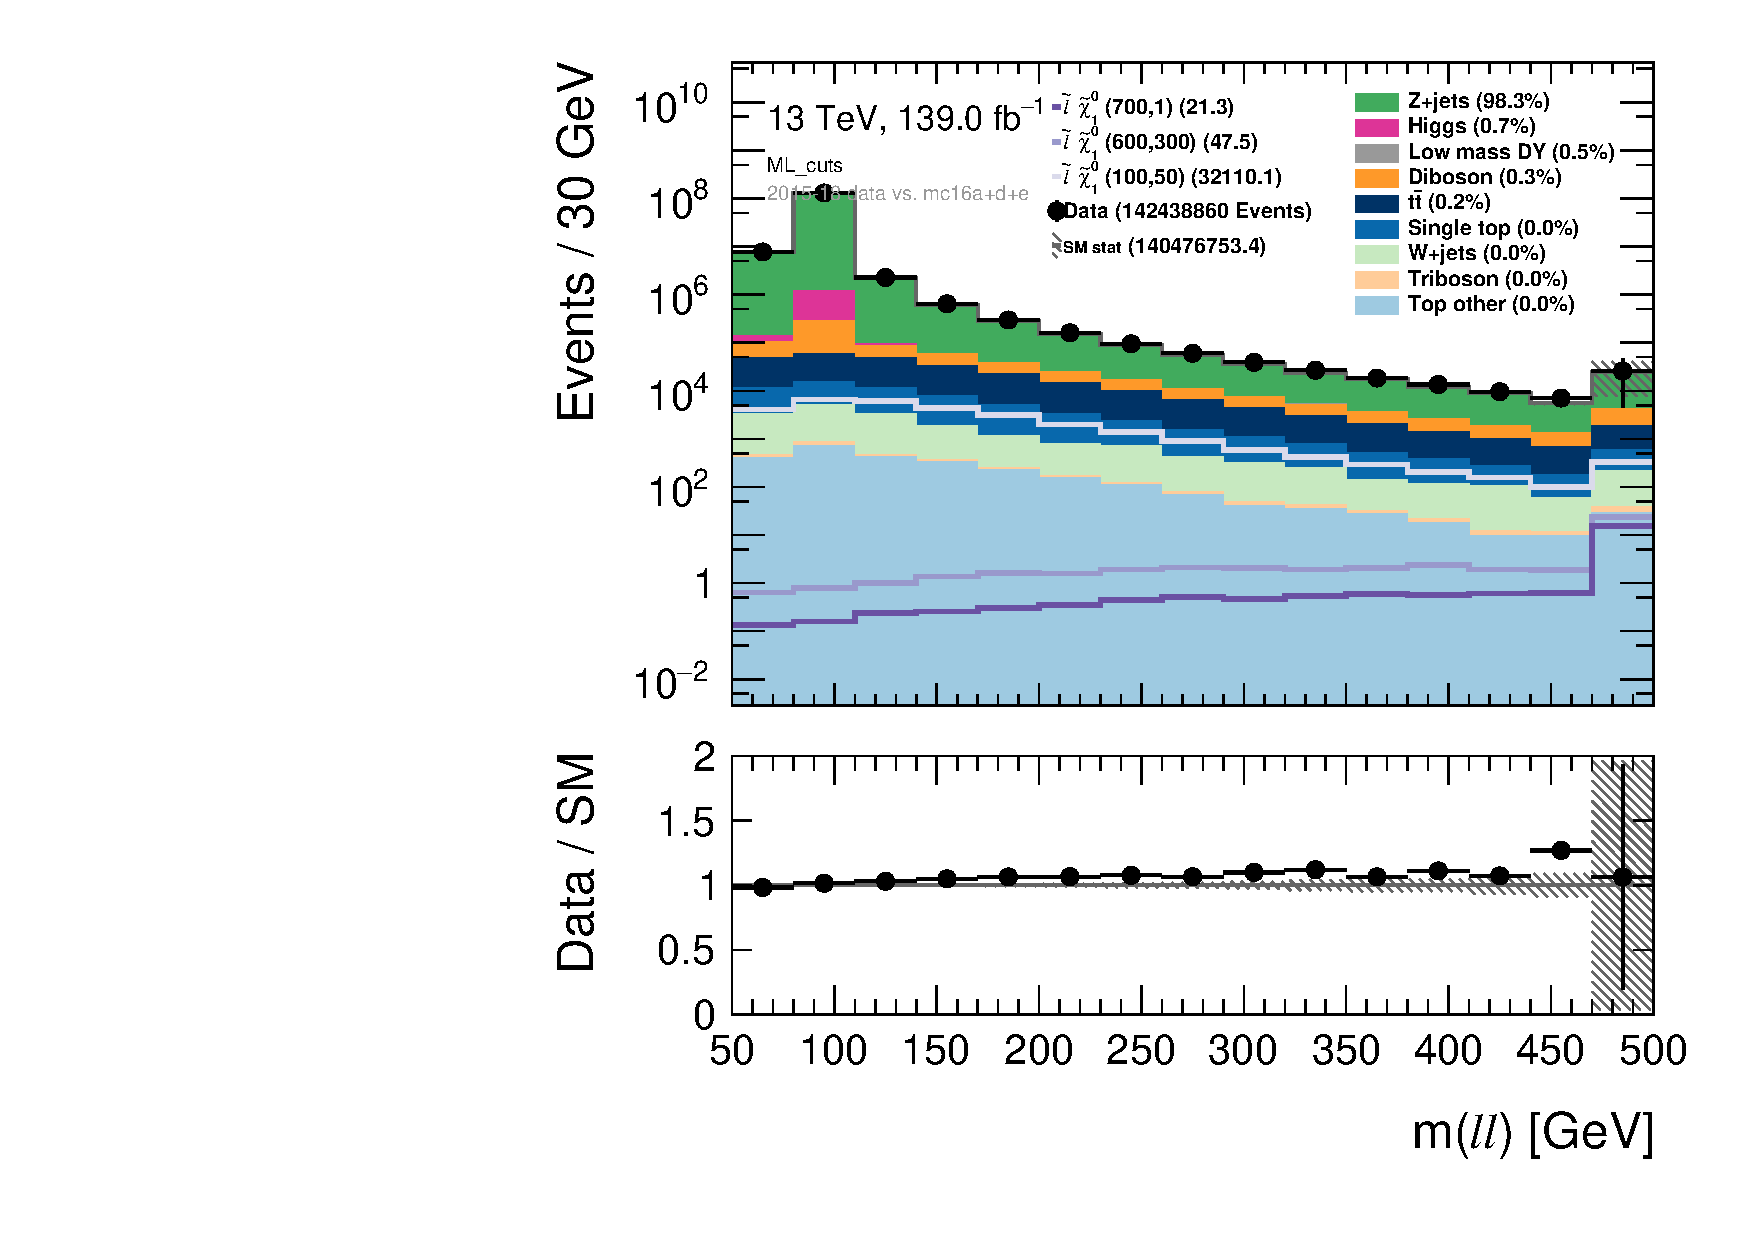
\includegraphics[width=\textwidth]{Figures/SlepSlep/CutAndCount/ML_cuts/hist1d_mll_ML_cuts.pdf}
    \caption{Invariant mass.}
    \label{fig:my_label}
    \end{subfigure}
    \begin{subfigure}[t!]{0.49\textwidth}
        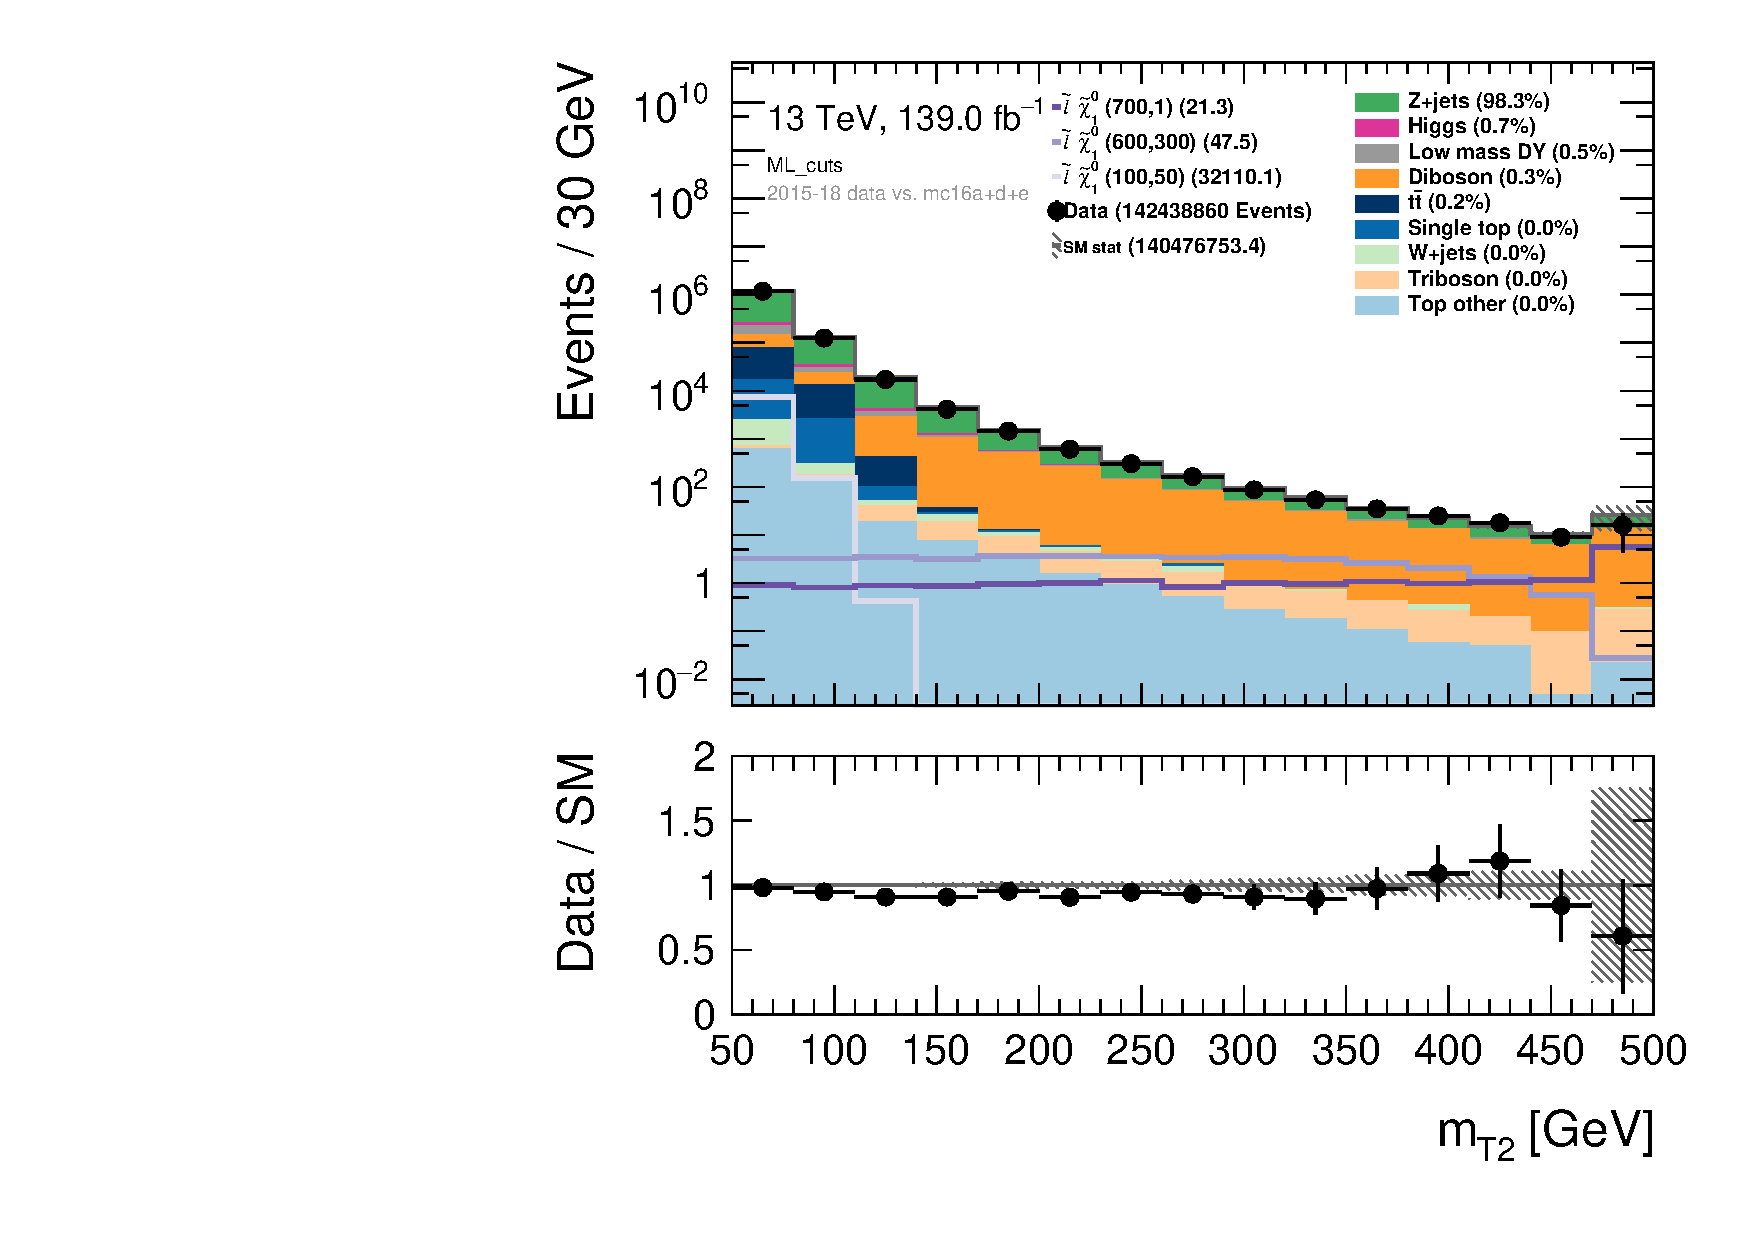
\includegraphics[width=\textwidth]{Figures/SlepSlep/CutAndCount/ML_cuts/hist1d_mt2_ML_cuts.pdf}
    \caption{Stransverse mass.}
    \label{fig:my_label}
    \end{subfigure}
        \caption{Plot of the different variables done with cut and count with the ML precuts as cuts.}
    \label{fig:ML_cuts}
\end{figure}

\restoregeometry

To make our ML analysis code more user friendly and unbiased (give the ML the opportunity to figure it out), we have used the same precuts for all four processes even though it might have been more efficiently to use some other precuts for the mono-Z process.

The goal with the ML analysis is to teach the computer to separate the signal from the background and then calculate the expected significance and compare it with the cut and count results. Since we are handling a huge amount of data and each step takes some time, we have separated some of the most time consuming steps to save some time to optimize the ML part. The first thing we did was to import all the nTuples, which are in rootfiles, and put them into pandas dataframes \footnote{Pandas dataframes \cite{PD} is a two-dimensional frame of your data which also includes the corresponding labels.}. Then we did all of the precuts in table \ref{tab:precutsSlepSlep}, giving the dataframes the features in table \ref{tab:features}, weighting and scaling up each event to correct luminosity from table \ref{tab:eventWeights} before we in the end stored all of the processed dataframes temporarily into HDF5 files \footnote{HDF5 \cite{hdf5} is a file format to store large, complex and heterogeneous data}. To avoid huge memory issues in the computer, this is done chunk by chunk since importing the whole dataset in one go are too much for our computers to handle. 

Importing the data is the most time consuming step, but luckily we don't have to do this every time we do some adjustments which is mainly done in the next part, the ML part. In the ML part we are training two different algorithms, namely a BDT and a NN. 

As mentioned in chapter \ref{sec:ML} we have to divide our input data into train and test sets, which are done by simply taking 1/3 of the input (randomly drawn) and call it the test set. This data is not going to be touched until we are finished with the training of our model except for 1/10 of the test set that are used for a validation set. To both save some time in the training and give the BDT and NN the opportunity to train more on actual signal samples, we have chosen to train on the same amount of background events as we have for signal. This gives us the results shown in figure \ref{fig:rawOutput}, which is the raw output from the trained model. This gives us an good indication on how much of our data that are needed to train a BDT or a NN. The reduction of the background doesn't have much impact on the results for the BDT except for some reduced training time, but for the NN the results improves a lot by doing this. 


\begin{figure}[H]
    \centering
    \begin{subfigure}[t!]{0.49\textwidth}
        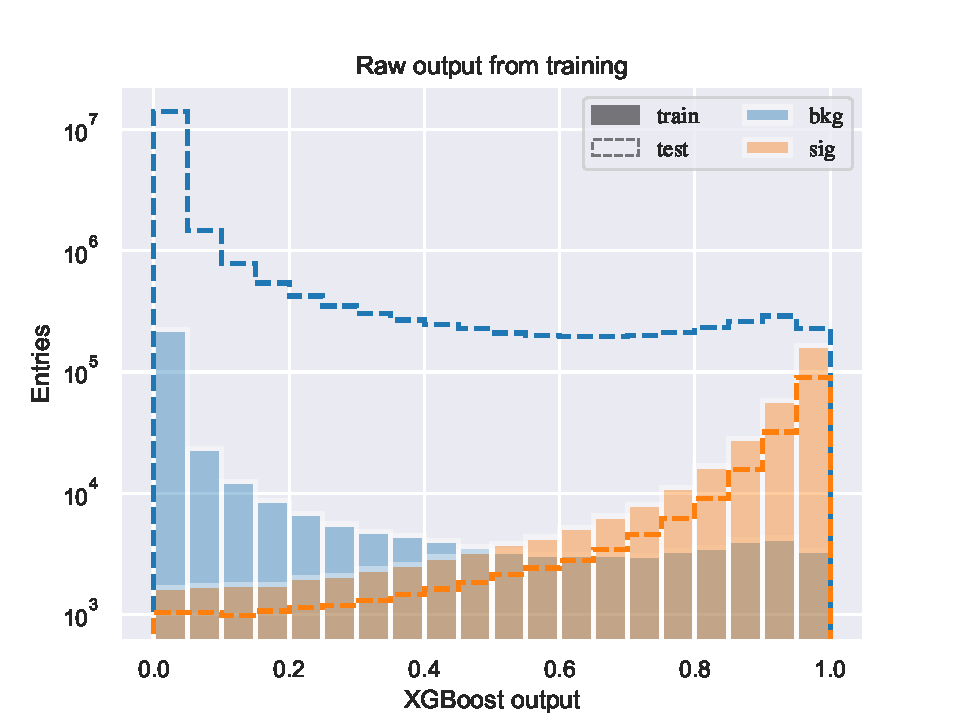
\includegraphics[width = \textwidth]{Figures/SlepSlep/ML/BDT/All_level/Low/rawPlot.pdf}
        \caption{A plot of the raw output from the BDT. This is obtained by using the signal samples from direct slepton production with low mass splitting and all level variables.}
        \label{fig:SlepSlepBDTLowLevelLowRaw}
    \end{subfigure}
    \begin{subfigure}[t!]{0.49\textwidth}
        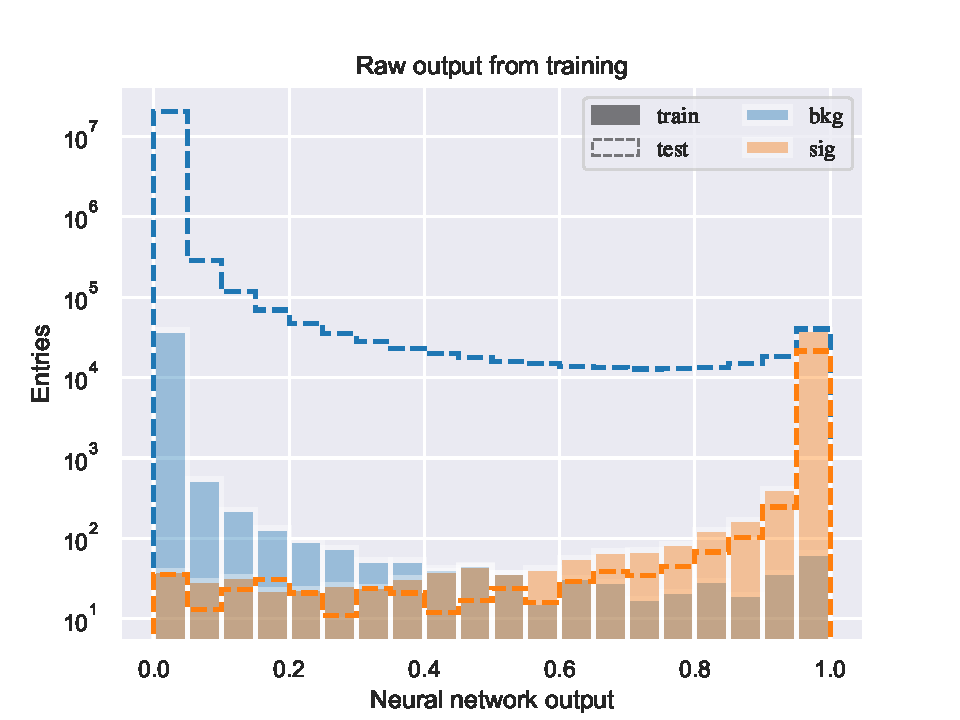
\includegraphics[width = \textwidth]{Figures/SlepSlep/ML/NN/All_level/High/rawPlot.pdf}
        \caption{A plot of the raw output from the NN. This is obtained by using the signal samples from direct slepton production with high mass splitting and all level variables.}
        \label{fig:SlepSlepNNLowLevelHighRaw}
    \end{subfigure}
    \caption{An example for both BDT and NN how the raw output looks after training and testing. These look pretty similar for all of the different processes and trained model and will therefore not be included in the thesis.}
    \label{fig:rawOutput}
\end{figure}



Since one signal sample alone is pretty small, we have merged the samples into different mass splittings. The reason for this is that with several together we get a lot more data to train our BDT and NN on and in this way our model will also handle other datasets much better. These mass splittings are chosen by the lines we have drawn in figure \ref{fig:exclusionPlots} in chapter \ref{sec:CandCanalysis}. Following the lines in figure \ref{fig:exclusionPlots} we get the mass splittings shown in table \ref{tab:massSplittings} for each process.

\begin{table}[H]
    \centering
    \renewcommand{\arraystretch}{1.3}
    \begin{tabular}{c c c c}
    \toprule
        \textbf{Process} & \textbf{Low} & \textbf{Intermediate} & \textbf{High}\\
        \midrule
        \midrule
        Direct slepton production & $\Delta$m $\leq$ 100 GeV & 100 $<$ $\Delta$m $<$450 GeV & $\Delta$m $\geq$ 450 GeV\\
        Chargino production via $\Tilde{l}/\Tilde{\nu}$& $\Delta$m $<$ 200 GeV & 200 $\leq$ $\Delta$m $<$600 GeV & $\Delta$m $\geq$ 600 GeV\\
        Chargino production via $W^\pm$ & $\Delta$m $<$ 150 GeV & 300 $\leq$ $\Delta$m $<$300 GeV & $\Delta$m $\geq$ 300 GeV\\
        Mono-Z & $\Delta$m $<$ 100 GeV & 100 $\leq$ $\Delta$m $<$350 GeV & $\Delta$m $\geq$ 350 GeV\\
        \bottomrule
    \end{tabular}
    \caption{Table of the different chosen mass splittings based on figure \ref{fig:exclusionPlots} for the different processes.}
    \label{tab:massSplittings}
\end{table}

%What signal sample that is in which category can also be found in the tables in \ref{sec:sigsamptab}.

When we are training the ML model we have some different results that can tell us how good or bad the model are doing. We can for example scale the test set up to be as big as the training set to see how good the fit is as shown in figure \ref{fig:traintestscaledExample}. We can also look at the ROC curve and AUC score, figure \ref{fig:ROCBDTLow_low_level}, to see how well the model can classify background as background and signal as signal. The goal in figure \ref{fig:traintestscaledExample} is that the test set (dotted line) is going to match the training set (filled bins) and in figure \ref{fig:ROCExample} we want an AUC-score of 1.

\begin{figure}[H]
    \centering
    \begin{subfigure}[t!]{0.49\textwidth}
        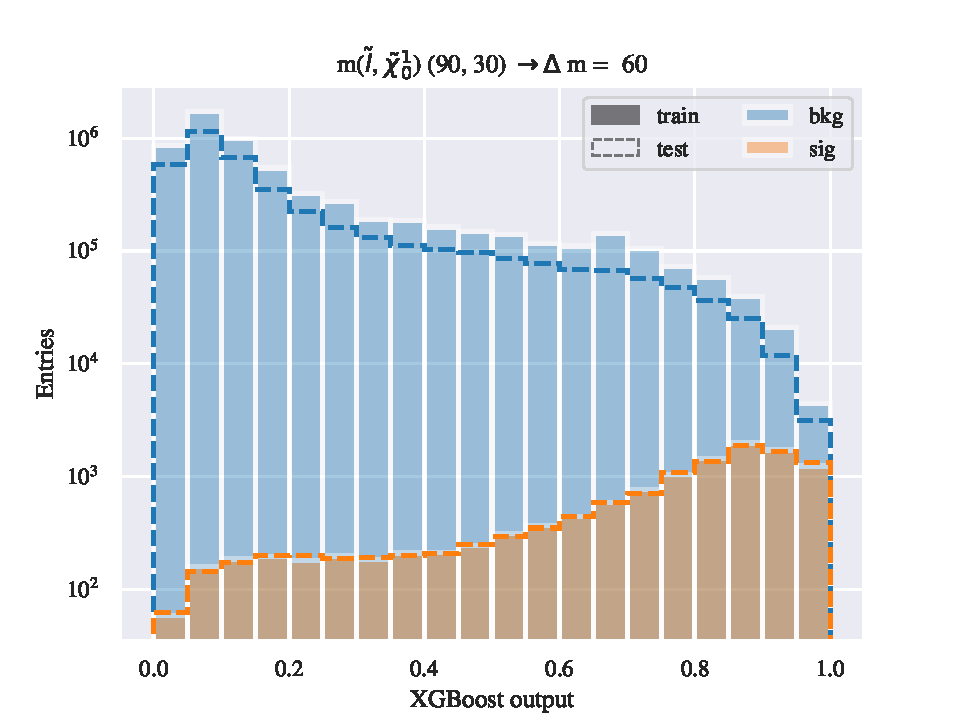
\includegraphics[width = \textwidth]{Figures/SlepSlep/ML/BDT/Low_level/Low/scaled_train_test_395897.pdf}
        \caption{A plot of the training and test set, where the test set is scaled up to match the training set.}
        \label{fig:traintestscaledExample}
    \end{subfigure}
    \begin{subfigure}[t!]{0.49\textwidth}
        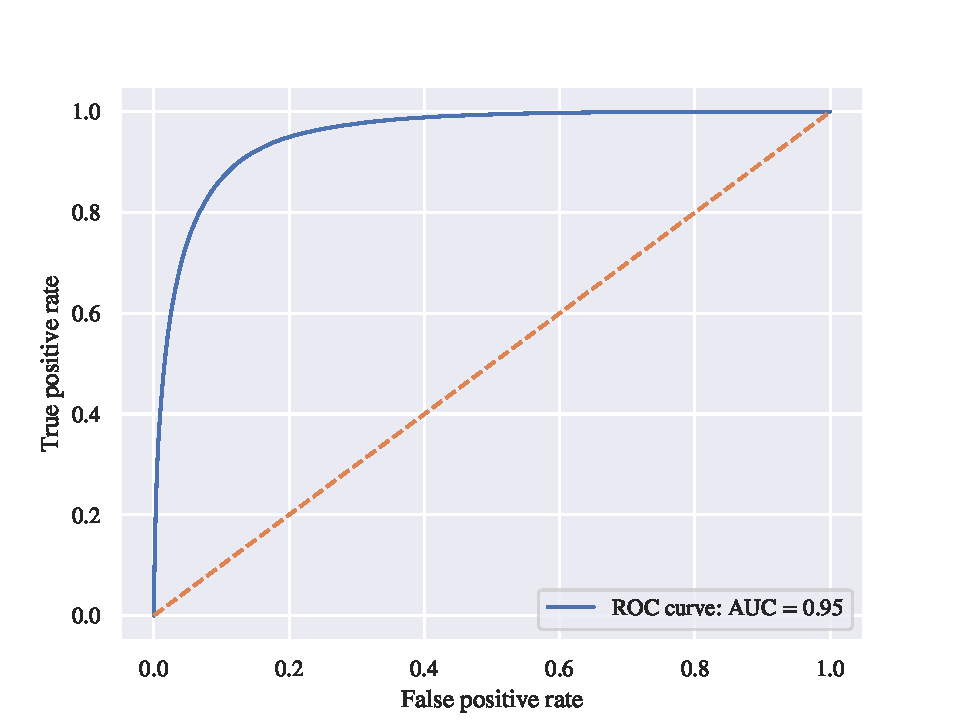
\includegraphics[width = \textwidth]{Figures/SlepSlep/ML/BDT/Low_level/Low/ROCcurve.pdf}
        \caption{A plot of the ROC curve together with the AUC score.}
        \label{fig:ROCExample}
    \end{subfigure}
    \caption{In this figure you can see results done by the BDT trained on low mass splittings and with low level variables for the direct slepton production.}
    \label{fig:resExample}
\end{figure}

Both of the plots in figure \ref{fig:resExample} is only included to have an example on what results we are judging the training on. The ROC-curve will not be shown for every trained model, but the AUC-score will be presented in a table for every trained model.

In addition to the ROC-curve and AUC-score, we have plotted the training loss vs the validation loss and the training accuracy vs the validation accuracy for the NN as shown in figure \ref{fig:resLossAccExample}. The loss should go towards zero and the accuracy towards one. 

\begin{figure}[H]
    \centering
    \begin{subfigure}[t!]{0.49\textwidth}
        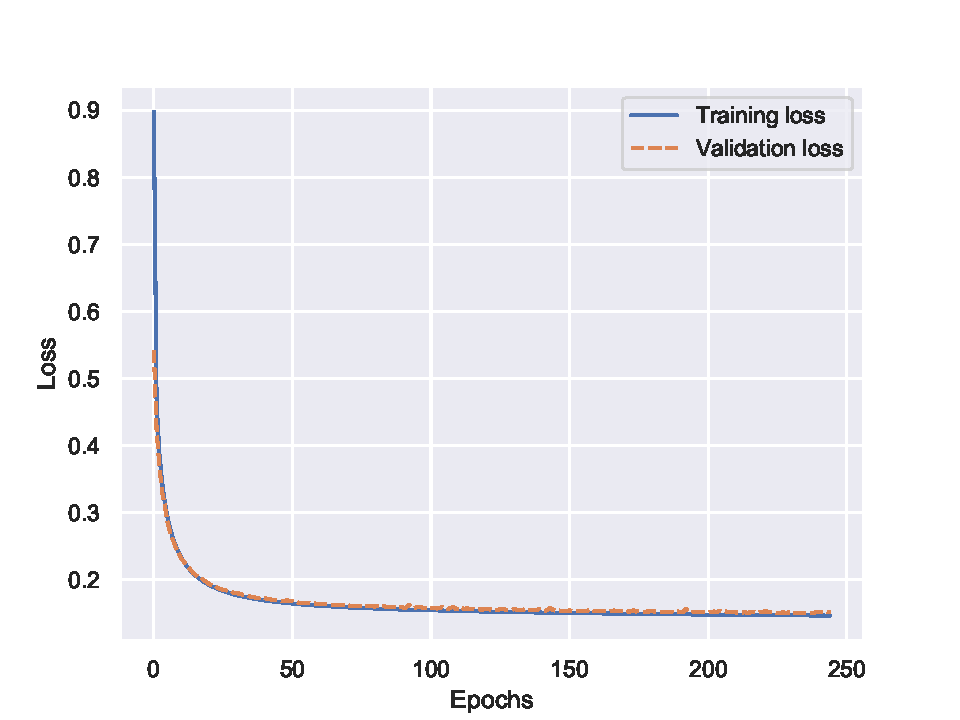
\includegraphics[width = \textwidth]{Figures/SlepSlep/ML/NN/High_level/Inter/Loss_sig_slepslep_high_level_inter.pdf}
        \caption{A plot of the training loss vs the validation loss.}
        \label{fig:LossExample}
    \end{subfigure}
    \begin{subfigure}[t!]{0.49\textwidth}
        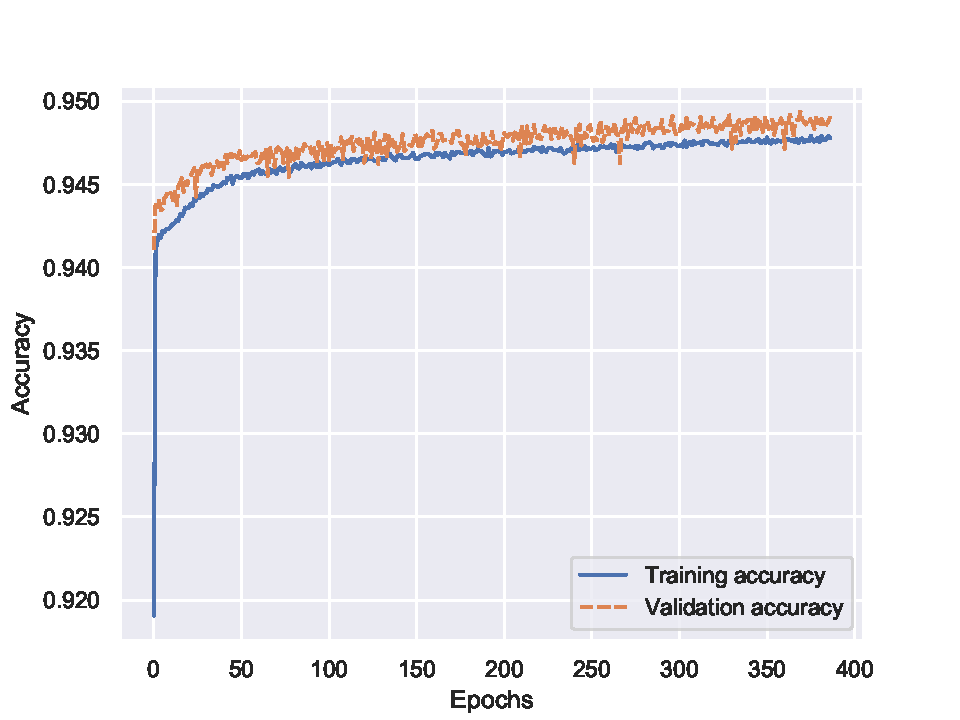
\includegraphics[width = \textwidth]{Figures/SlepSlep/ML/NN/High_level/Inter/Accuracy_sig_slepslep_high_level_inter.pdf}
        \caption{A plot of the training accuracy vs validation accuracy.}
        \label{fig:AccExample}
    \end{subfigure}
    \caption{In this figure we can see results done by the NN trained on intermediate mass splittings and with high level variables for the direct slepton production.}
    \label{fig:resLossAccExample}
\end{figure}

As we can see in figure \ref{fig:LossExample}, both the training and validation loss goes pretty fast towards zero after the NN starts training and does not improve much after $\sim 100$ epochs. This means that we probably could have stopped the training after only 100 epochs and still gotten a fairly good result, but we want the best result as possible and therefore we let it minimize the loss some more. We can also see that the validation loss is constantly flat in the end and would not improve anymore (continue towards zero), while the training loss continues down towards zero. If we have not stopped after 10 steps (which is the patience we have given the early stopping function, while the BDT have a patience on 20 steps) of no improvement, the validation loss would have started to go a bit up again away from zero. This is not that easy to see in this plot, but same point is in the accuracy plot in figure \ref{fig:AccExample}, where we can see this more clearly. It is a bit hard to determine if the validation accuracy tends to go down again because of the fluctuations\footnote{The fluctuations can be avoided by having a bigger validation set, but then you will also have a smaller test set to test your ML model on.}, but it is fairly easy to see that the training accuracy continue towards one. That the training loss and accuracy continues to improve is often due to overtraining/overfitting which we want to avoid.

The plots in figure \ref{fig:resLossAccExample} for every process will not be presented in this thesis since they are going to look very similar for every process and ensemble of training compositions.


\section{Building, training and testing the BDT}
Now we know how a BDT and NN works and we are prepared on what we can expect of results. In this section we will get an understanding on how the BDT are built up, how we train it and, in the end, testing how well the training went.

\subsection{Building}
The BDT, as mentioned in chapter \ref{sec:BDT}, is built up using a existing python library called XGBoost. The variables I have to care about are listed in table \ref{tab:parametersBDT} below. 


%To obtain the results in figure \ref{fig:SlepSlepBDTLowLevelLowRaw} we have given the BDT some parameters which are listed in table \ref{tab:parametersBDT}. These parameters is simply found by trial and error with of course an indication on what magnitude we are going to be within. 

\begin{table}[H]
    \centering
    \renewcommand{\arraystretch}{1.}
    \begin{tabular}{c c}
    \toprule
    \textbf{Parameter} & \textbf{Value}\\
    \midrule
    \midrule
    Maximum depth of tree & 3\\
    Learning rate     & 0.1 \\
    Number of estimators     & 10000000\\
    Verbosity & 3\\
    Objective & binary:logistic\\
    Scale position weight & 1\\
    \bottomrule
    \end{tabular}
    \caption{An overview of the different parameters used during training to obtain the results for the BDT.}
    \label{tab:parametersBDT}
\end{table}

Most of these parameters are self explanatory, but not all of them so we will take a brief explanation before we move on. The first parameter that is not so intuitive is the verbosity level, which we set to let the BDT how much information we want from the tree during training. This can be set at 0, 1, 2 or 3, where 0 is silent, 3 is debug and 1 and 2 will give us parts of the information. It is nice to see what is going on during the training, so we have chosen to set it to 3. The next parameter we are going to explain is the objective, which specifies the learning task we are doing and the learning objective. As we can see in table \ref{tab:parametersBDT}, we have chosen to use something called \texttt{binary:logistic} which simply is a logistic regression for a binary classification. And last, we have the scale position weight which controls the balance between negative and positive weights in the tree. 

In addition to the parameters that we have to give the BDT, we have different compositions of models we are training. As mentioned earlier in this chapter we are training on three different mass splittings (low, intermediate and high), but we are also training on high level, low level or all the features we listed up in table \ref{tab:features}. This is done to see how important the different features are during the next step, namely the training.

\subsection{Training}
While we train our BDT, we have to be aware of overtraining/overfitting. This can easily be done by putting in a demand on the loss and stop the training early. This is simply done by calculating the loss from the validation set and give the BDT a patience parameter on 20 steps and it will stop if the loss haven't improved in 20 steps and save the model made at the best iteration. This is also the reason for the high number of estimators in table \ref{tab:parametersBDT}. 

It is not much more we can do while the BDT are training, other than wait to see how the testing looks. If we are not happy with how the model is trained, we have to go back to the building of the tree and adjust the parameters in table \ref{tab:parametersBDT} and do the training again until we are happy with our results.

\subsection{Testing}
The last step of the BDT is to test it on the test set. We have a lot of results from the BDT to look at since we have trained the model with low, intermediate and high mass splittings and with high level, low level and all features for four different processes. We are going to look at all 4 processes at the same time and see how the results evolves with changing the features and mass splittings. All of the results that are not shown in this chapter can be found in the appendix \ref{sec:appBDTplots}. 

\subsubsection{AUC score}
The main selection of results is done based on the AUC-score. If the AUC-score is the same for high level, low level and all features, we have made the decision on looking at which features that have been important for the trained model. The AUC-scores are listed in table \ref{tab:AUCBDT}. 

\begin{table}[H]
    \centering
    \renewcommand{\arraystretch}{1.}
    \begin{tabular}{l l c c c c }
    \toprule
    \textbf{Level} & $\mathbf{\Delta m}$ & $\mathbf{\Tilde{l} \Tilde{l}}$ & $\mathbf{\Tilde{\chi}_1^\pm \rightarrow \Tilde{l}/\Tilde{\nu}}$ & $\mathbf{\Tilde{\chi}_1^\pm \rightarrow W^\pm}$ & \textbf{Mono-Z}  \\
    \midrule
    \midrule
    \multirow{3}{*}{High} &  Low   & 0.92 & 0.92 & 0.91 & 0.95 \\
     & Intermediate & 0.99 & 0.98 & 0.94 & 0.96 \\
     & High & 1.00 & 1.00 & 0.96 & 0.97 \\
     \midrule
    \multirow{3}{*}{Low} & Low & 0.93 & 0.92 & 0.92 & 0.93 \\
     & Intermediate & 0.99 & 0.98 & 0.95 & 0.96 \\
     & High & 1.00 & 1.00 & 0.97 & 0.96 \\
     \midrule
    \multirow{3}{*}{All} & Low & 0.95 & 0.94 & 0.94 & 0.96 \\
     & Intermediate & 1.00 & 0.99 & 0.96 & 0.97 \\
     & High & 1.00 & 1.00 & 0.98 & 0.98 \\
     \bottomrule
    \end{tabular}
    \caption{The AUC score for all four processes with different compositions of features and mass splittings for the BDT.}
    \label{tab:AUCBDT}
\end{table}


As we can see in table \ref{tab:AUCBDT}, the preferred composition of features is almost constantly to use all the features, except for some few exceptions where all three options have the same AUC-score. As mentioned above, this then determined by looking at the feature importance plot that also are presented in the following sections. The results are presented for each mass splitting with all the processes together for easier comparison. The signal samples that are chosen is the same ones we have looked at in the cut and count analysis earlier in this thesis.
















\subsubsection{Low mass splittings}
The first results from the BDT is for the BDTs trained on low mass splittings. The preferred composition of features is all features and in figure \ref{fig:AllLowfeatBDT} we can see how these different features contributes during training. 


\begin{figure}[H]
    \centering
    \begin{subfigure}[t!]{0.49\textwidth}
        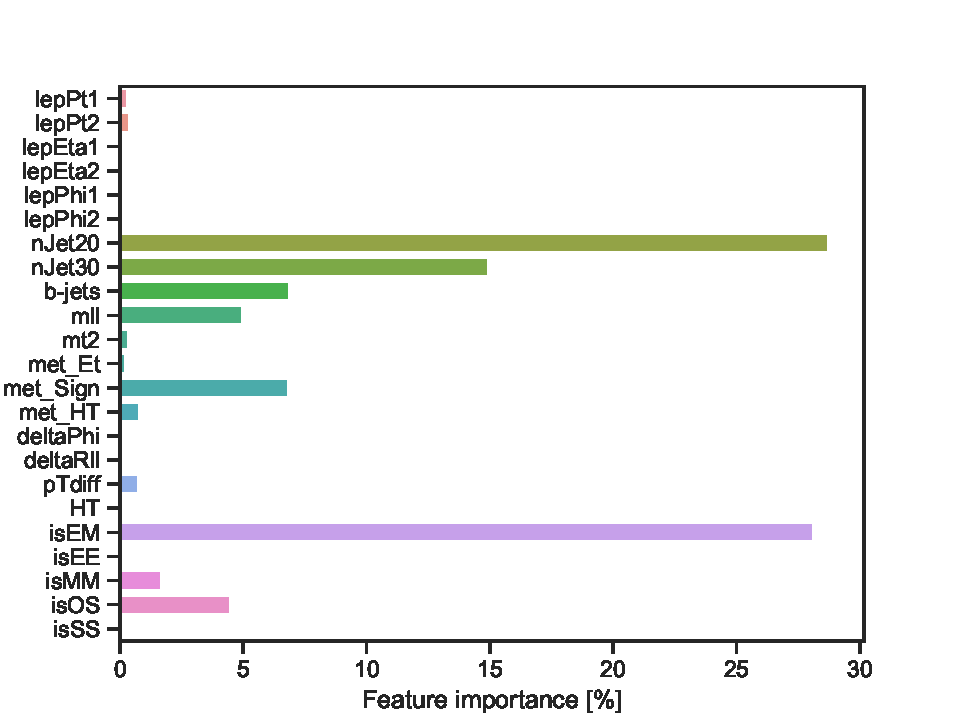
\includegraphics[width = \textwidth]{Figures/SlepSlep/ML/BDT/All_level/Low/featureImportance.pdf}
        \caption{Direct slepton production.}
        \label{fig:featSlepslepLow}
    \end{subfigure}
    \begin{subfigure}[t!]{0.49\textwidth}
        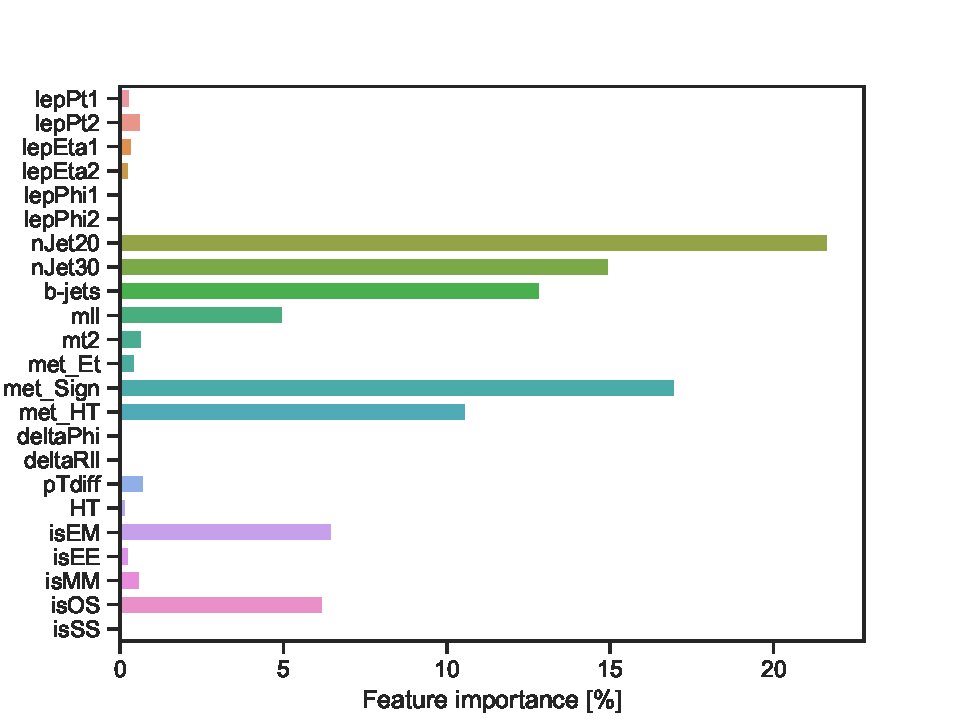
\includegraphics[width = \textwidth]{Figures/SlepSnu/BDT/All_level/Low/featureImportance.pdf}
        \caption{Chargino production via $\Tilde{l}/\Tilde{\nu}$.}
        \label{fig:featSlepsnuLow}
    \end{subfigure}
    \begin{subfigure}[t!]{0.49\textwidth}
        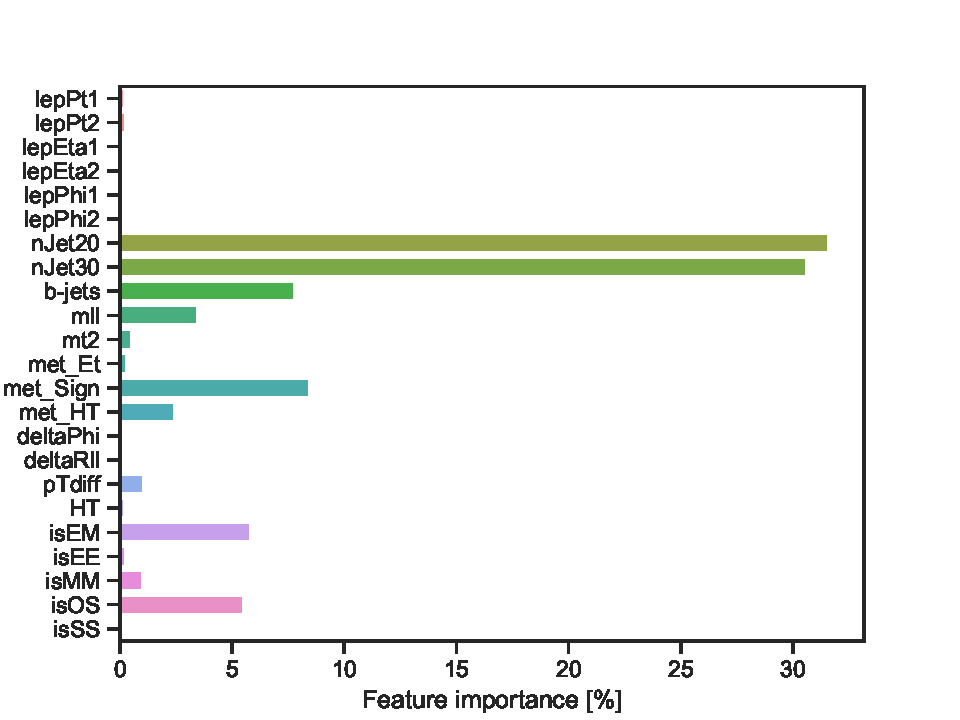
\includegraphics[width = \textwidth]{Figures/WW/BDT/All_level/Low/featureImportance.pdf}
        \caption{Chargino production via $W^\pm$.}
        \label{fig:featWWLow}
    \end{subfigure}
    \begin{subfigure}[t!]{0.49\textwidth}
        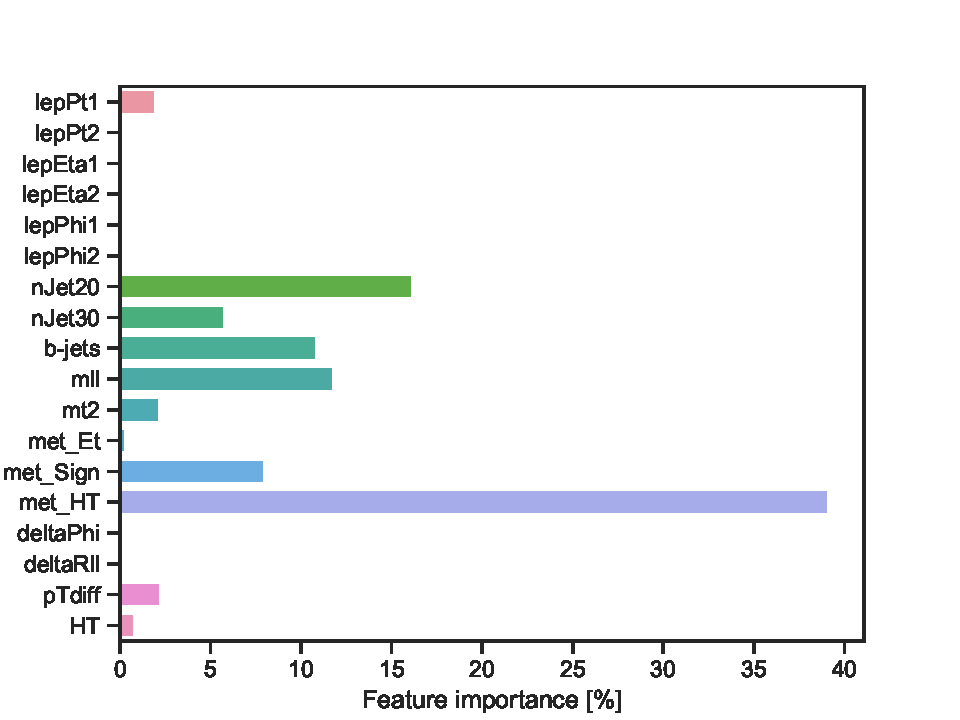
\includegraphics[width = \textwidth]{Figures/Mono_Z/ML/BDT/All_level/Low/featureImportance.pdf}
        \caption{Mono-Z.}
        \label{fig:featMonoZLow}
    \end{subfigure}
    \caption{Feature importance for low mass splittings for all four processes using all features during training.}
    \label{fig:AllLowfeatBDT}
\end{figure}

If we now look at the different feature contributions in figure \ref{fig:AllLowfeatBDT}, we can see that jets with a $p_T > 20$ GeV is an important feature while the BDT is training on the SUSY processes. This means that the BDT thinks this is a good variable to distinguish the signal from the background on, which again can be drawn back to the cut and count analysis, where we already do a cut on jets. The BDT tells us that this is most likely a good variable to look at for the SUSY processes when trying to separate the signal from the background. In addition we can see that the jets with a $p_T > 30$ GeV, b-jets, $m_{ll}$ and MET significance have been used a lot. This is also variables we have used when doing the cut and count analysis, but they does not contribute equally much for every SUSY process. For the mono-Z process, it have mainly used the same features as for the SUSY processes, but MET/$H_T$ have definitely been the most important one. This can also be drawn back to the cut and count analysis where we do a cut on this variable as well. To conclude the feature importance for low mass splittings we can say that it is not any very big surprises when thinking of the cuts done in cut and count.

The next step is to see how well the testing of the model went. This can be seen in figure \ref{fig:AllLowBDT} below.

\begin{figure}[H]
    \centering
    \begin{subfigure}[t!]{0.49\textwidth}
        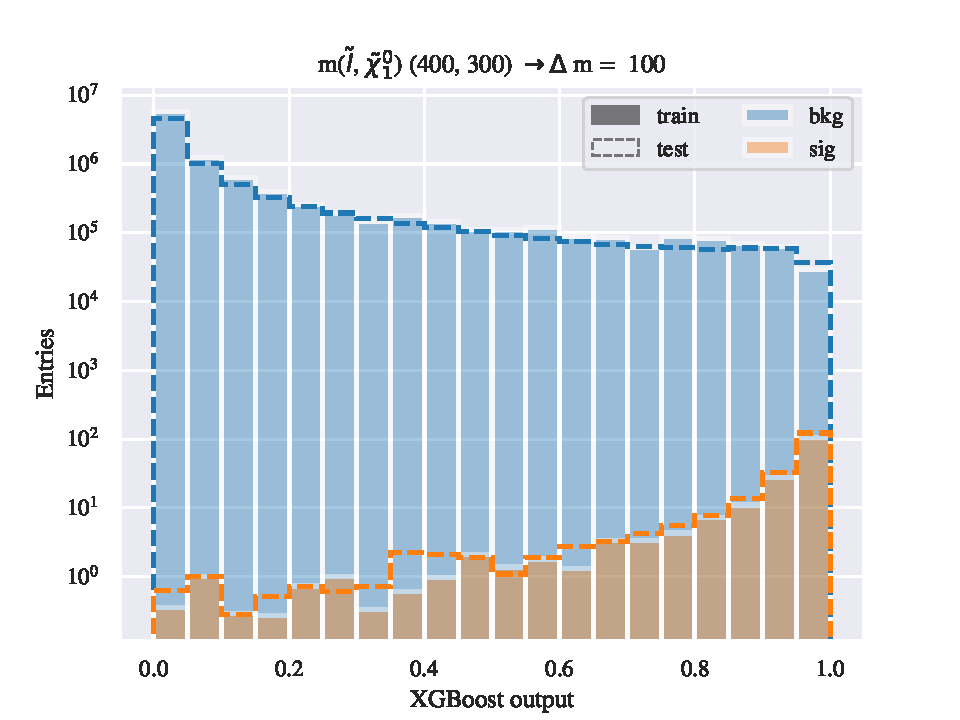
\includegraphics[width = \textwidth]{Figures/SlepSlep/ML/BDT/All_level/Low/scaled_train_test_395984.pdf}
        \caption{Direct slepton production.}
        \label{fig:SlepslepLow}
    \end{subfigure}
    \begin{subfigure}[t!]{0.49\textwidth}
        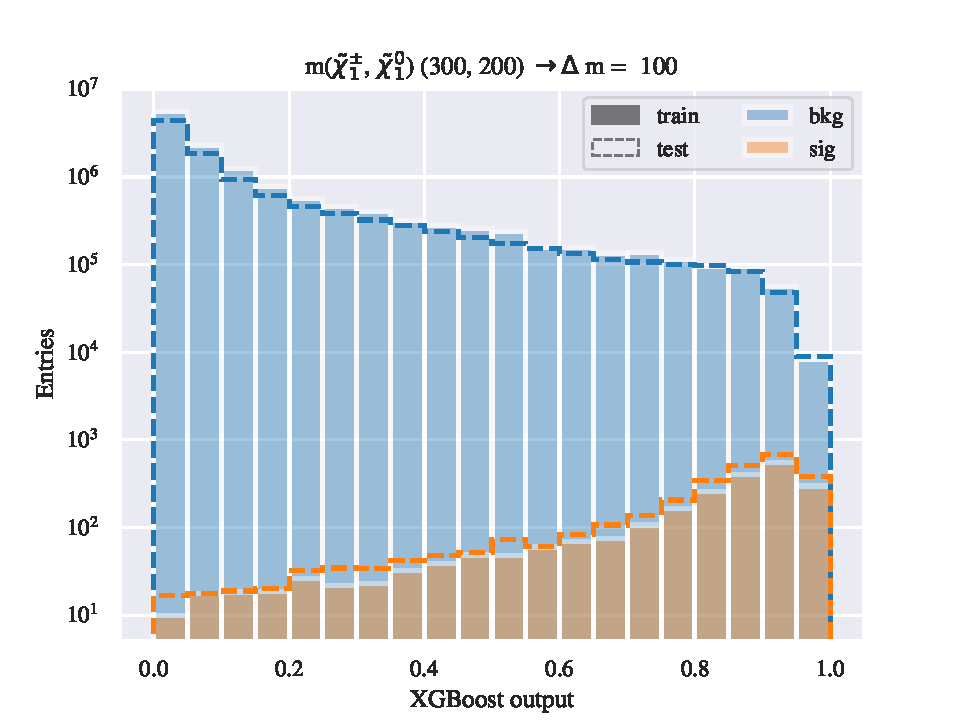
\includegraphics[width = \textwidth]{Figures/SlepSnu/BDT/All_level/Low/scaled_train_test_397115.pdf}
        \caption{Chargino production via $\Tilde{l}/\Tilde{\nu}$.}
        \label{fig:SlepsnuLow}
    \end{subfigure}
    \begin{subfigure}[t!]{0.49\textwidth}
        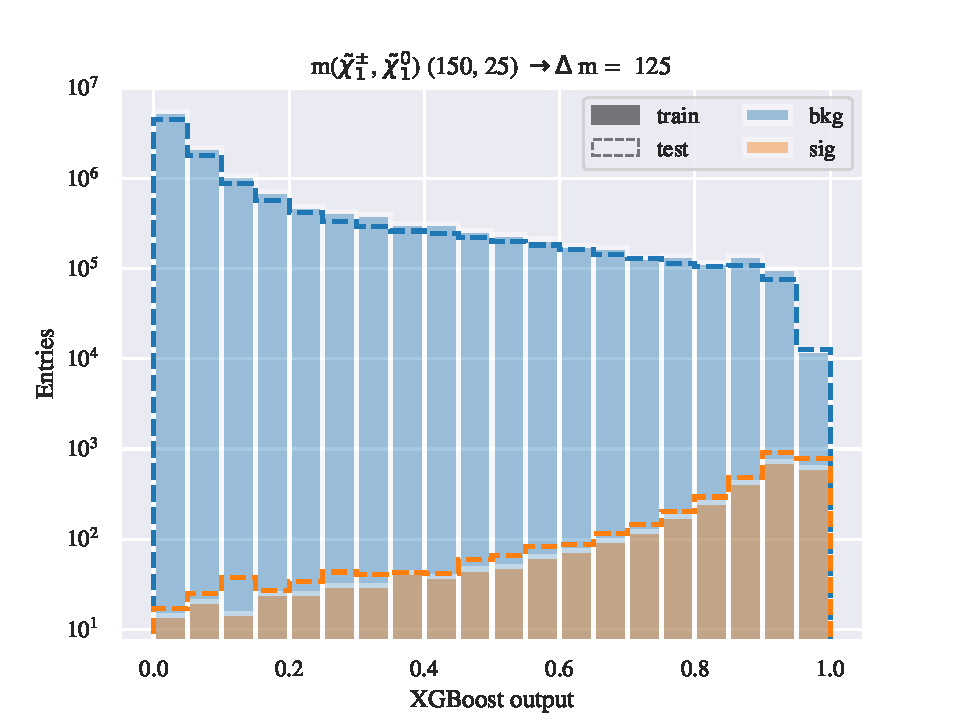
\includegraphics[width = \textwidth]{Figures/WW/BDT/All_level/Low/scaled_train_test_395268.pdf}
        \caption{Chargino production via $W^\pm$.}
        \label{fig:WWLow}
    \end{subfigure}
    \begin{subfigure}[t!]{0.49\textwidth}
        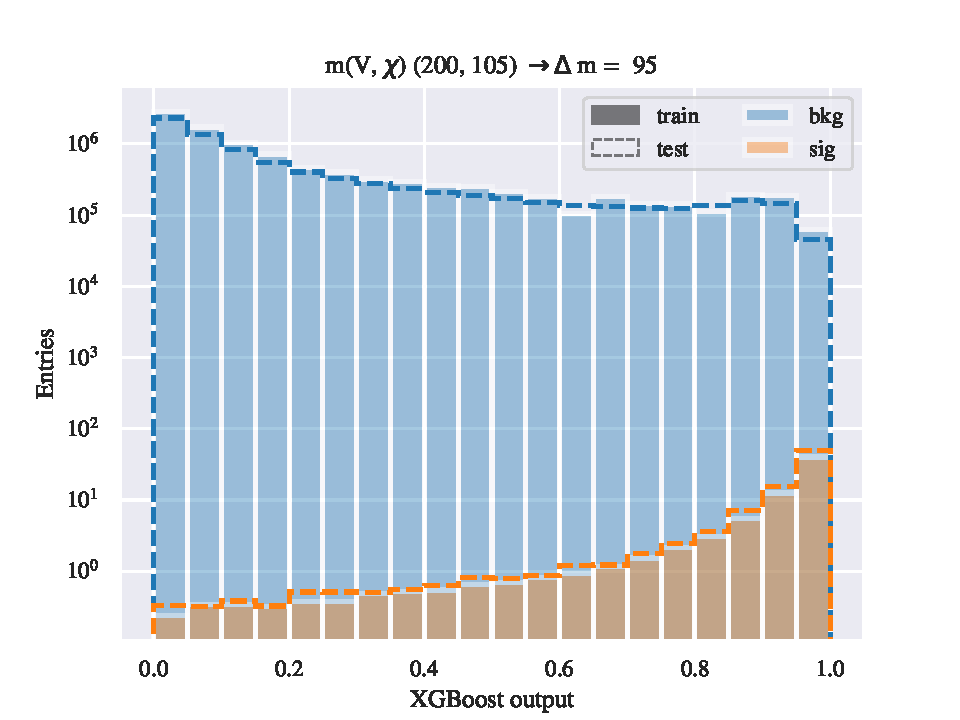
\includegraphics[width = \textwidth]{Figures/Mono_Z/ML/BDT/All_level/Low/scaled_train_test_310604.pdf}
        \caption{Mono-Z.}
        \label{fig:MonoZLow}
    \end{subfigure}
    \caption{Test vs train for low mass splittings done with the BDT. Here the test set is scaled up to match the number of training events.}
    \label{fig:AllLowBDT}
\end{figure}

As we can see in figure \ref{fig:AllLowBDT}, the test set (dashed line) match the training set pretty well for all processes. It differs a bit some places, but overall it is a good fit. We can also see that the mass splitting is not that good, but it is at least most signal up to one which is the value we have labeled the signal as. That the separation is this poorly is because of the masses we are looking at are mostly among the masses to the particles in the SM which makes them harder to separate. This is a known problem in high energy particle physics and is something we hopefully will find a good way to figure out one day. 



























\subsubsection{Intermediate mass splittings}

The next mass splitting we are looking at is the intermediate mass splittings. In figure \ref{fig:featAllInterBDT} we can see the importance of the different features where all features are used for training. 

\begin{figure}[H]
    \centering
    \begin{subfigure}[t!]{0.49\textwidth}
        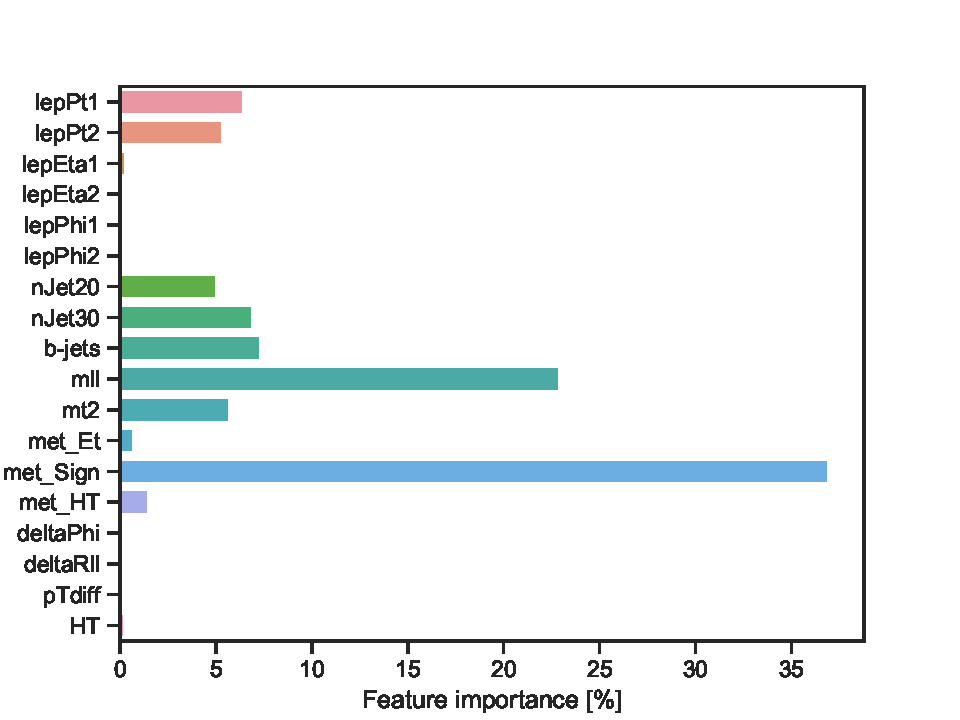
\includegraphics[width = \textwidth]{Figures/SlepSlep/ML/BDT/All_level/Inter/featureImportance.pdf}
        \caption{Direct slepton production.}
        \label{fig:featSlepslepInter}
    \end{subfigure}
    \begin{subfigure}[t!]{0.49\textwidth}
        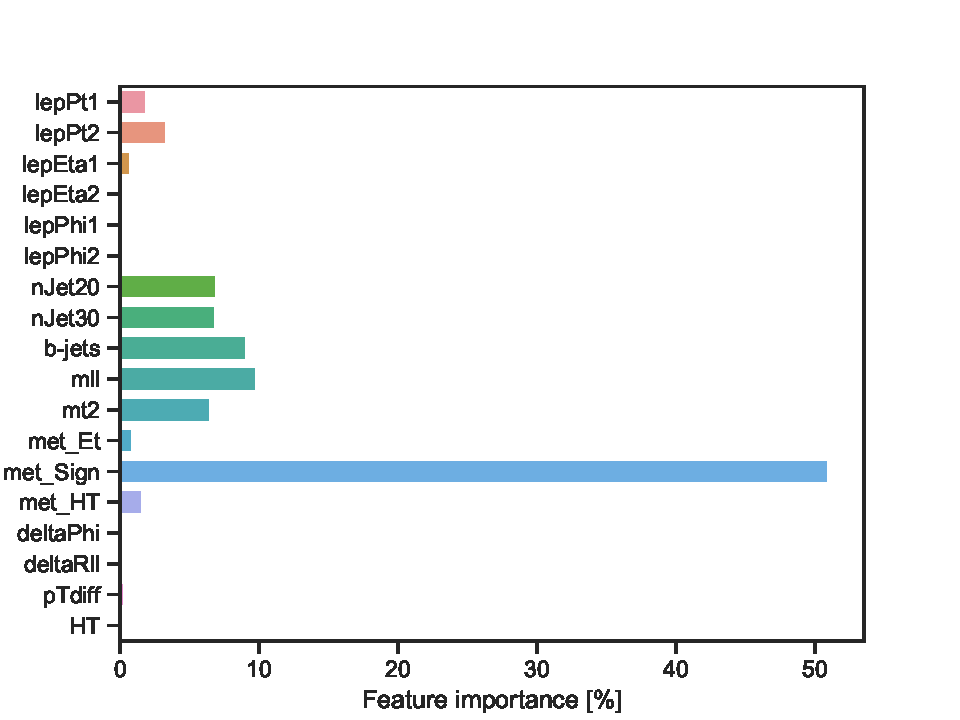
\includegraphics[width = \textwidth]{Figures/SlepSnu/BDT/All_level/Inter/featureImportance.pdf}
        \caption{Chargino production via $\Tilde{l}/\Tilde{\nu}$.}
        \label{fig:featSlepsnuInter}
    \end{subfigure}
    \begin{subfigure}[t!]{0.49\textwidth}
        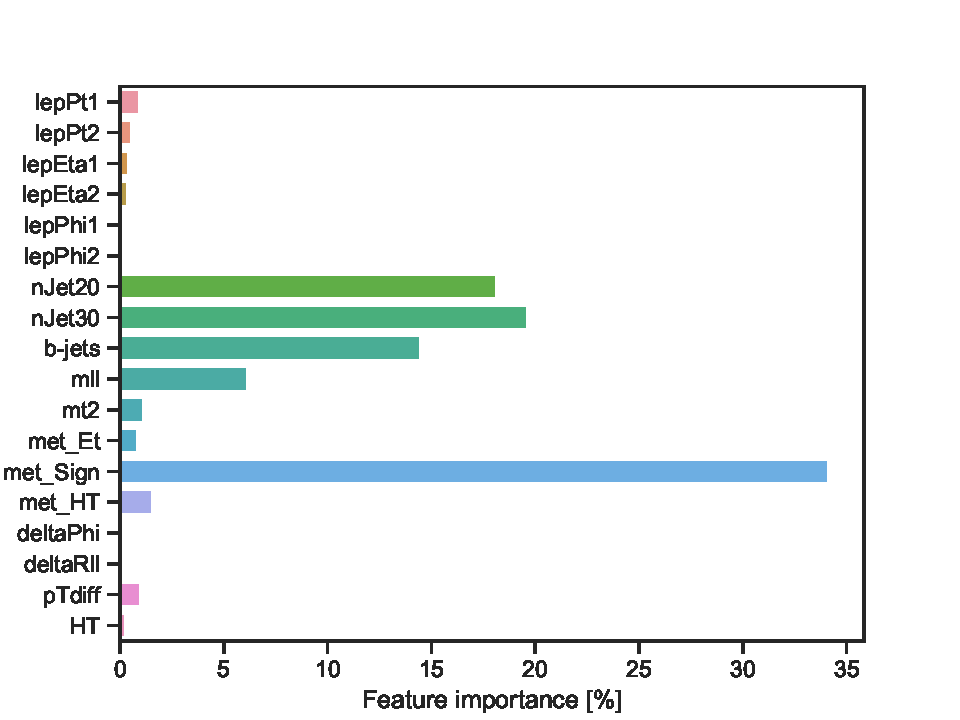
\includegraphics[width = \textwidth]{Figures/WW/BDT/All_level/Inter/featureImportance.pdf}
        \caption{Chargino production via $W^\pm$.}
        \label{fig:featWWInter}
    \end{subfigure}
    \begin{subfigure}[t!]{0.49\textwidth}
        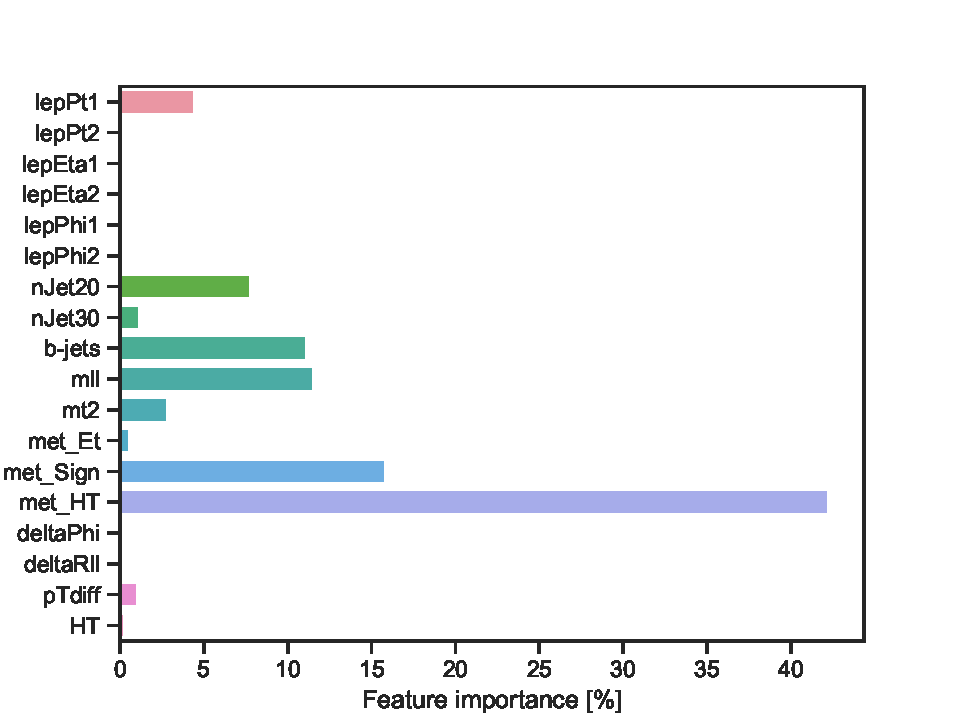
\includegraphics[width = \textwidth]{Figures/Mono_Z/ML/BDT/All_level/Inter/featureImportance.pdf}
        \caption{Mono-Z.}
        \label{fig:featMonoZInter}
    \end{subfigure}
    \caption{Feature importance for intermediate mass splittings for all four processes using all features during training.}
    \label{fig:featAllInterBDT}
\end{figure}

In figure \ref{fig:featAllInterBDT} we can see that MET significance is the most important feature for the SUSY processes and the second most important feature for mono-Z. This might be a bit more interesting result than for the low mass splittings, since we, in cut and count, do a very gentle cut on this variable while the BDT finds it very interesting while training. For later work on a similar analysis, this could be interesting to test in the cut and count analysis as well. The other features the BDT finds interesting, for all four processes, is more or less the same as for low mass splittings. 

\begin{figure}[H]
    \centering
    \begin{subfigure}[t!]{0.49\textwidth}
        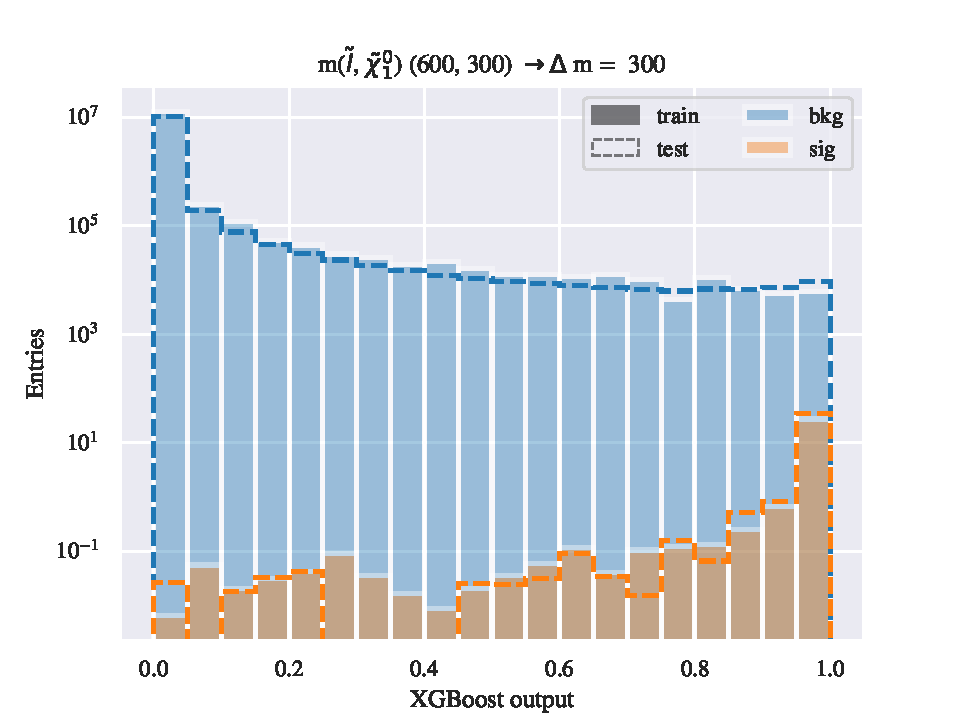
\includegraphics[width = \textwidth]{Figures/SlepSlep/ML/BDT/All_level/Inter/scaled_train_test_396014.pdf}
        \caption{Direct slepton production.}
        \label{fig:SlepslepInter}
    \end{subfigure}
    \begin{subfigure}[t!]{0.49\textwidth}
        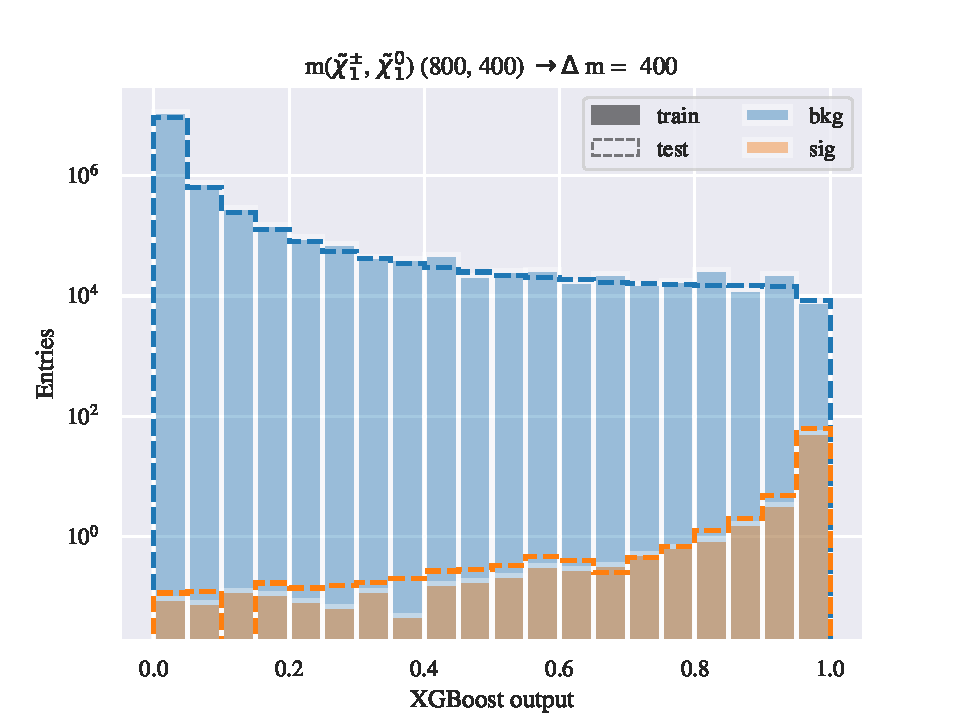
\includegraphics[width = \textwidth]{Figures/SlepSnu/BDT/All_level/Inter/scaled_train_test_397150.pdf}
        \caption{Chargino production via $\Tilde{l}/\Tilde{\nu}$.}
        \label{fig:SlepsnuInter}
    \end{subfigure}
    \begin{subfigure}[t!]{0.49\textwidth}
        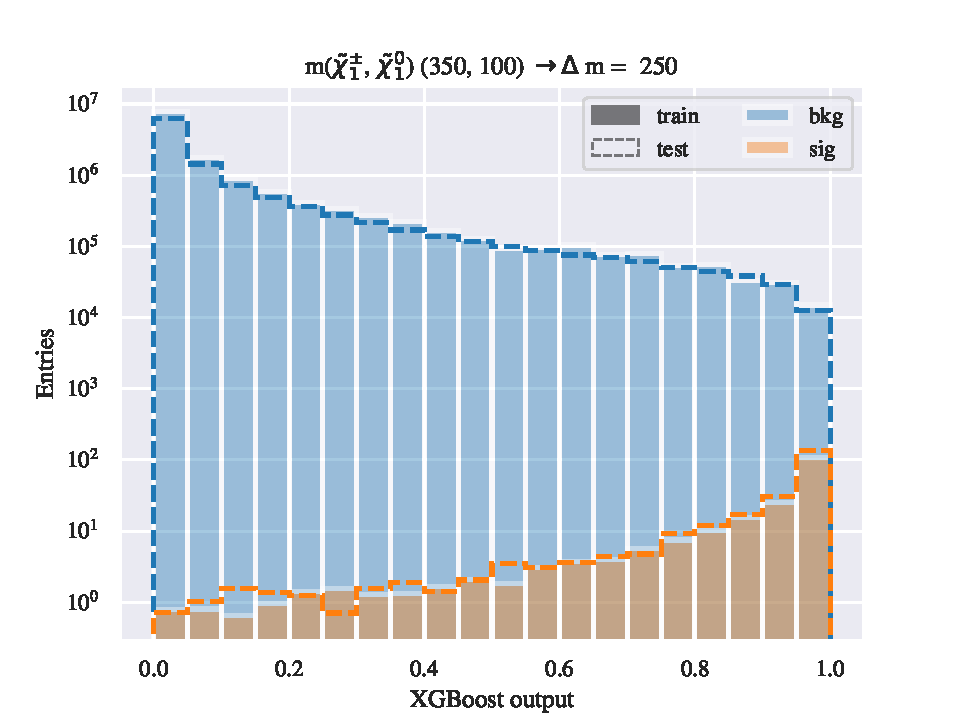
\includegraphics[width = \textwidth]{Figures/WW/BDT/All_level/Inter/scaled_train_test_395320.pdf}
        \caption{Chargino production via $W^\pm$.}
        \label{fig:WWInter}
    \end{subfigure}
    \begin{subfigure}[t!]{0.49\textwidth}
        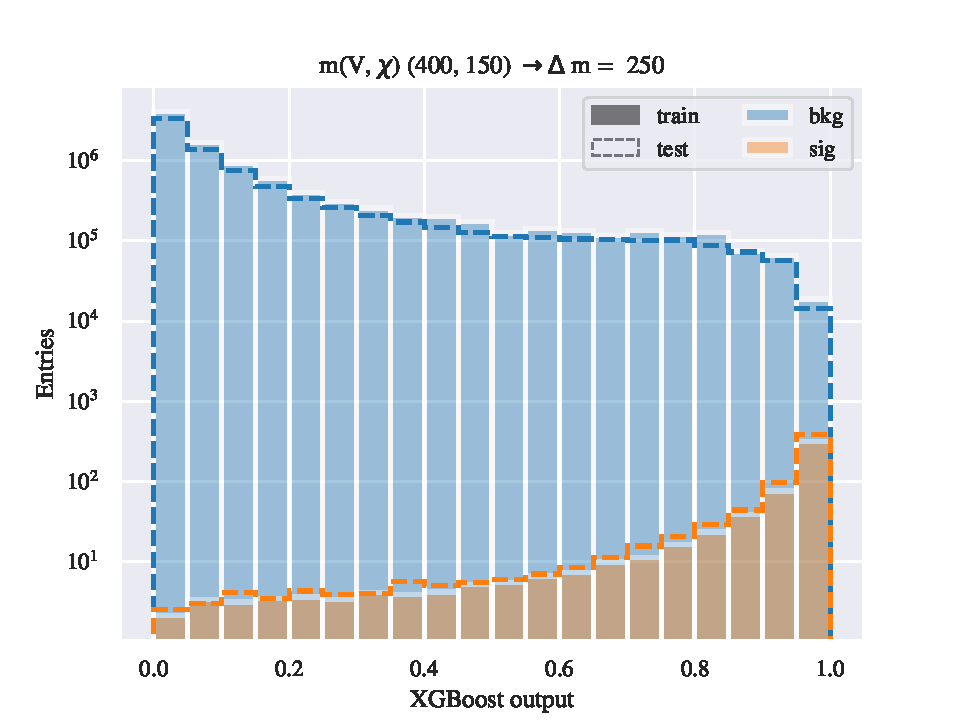
\includegraphics[width = \textwidth]{Figures/Mono_Z/ML/BDT/All_level/Inter/scaled_train_test_310613.pdf}
        \caption{Mono-Z.}
        \label{fig:MonoInter}
    \end{subfigure}
    \caption{Test vs train for intermediate mass splittings done with the BDT. Here the test set is scaled up to match the number of training events.}
    \label{fig:AllInterBDT}
\end{figure}

The results from testing the trained model is shown in figure \ref{fig:AllInterBDT}. As we could see for the low mass splittings, it is overall a pretty good match. We can also see that we have a bit more signal up to one and a bit less background in this region. This is not that surprising considering that we are now moving away from the masses within the SM. 
















\subsubsection{High mass splittings}

The last BDT we have trained is the one trained on high mass splittings. Here we can see some interesting change in the importance of the different features in figure \ref{fig:AllHighfeatBDT}.

\begin{figure}[H]
    \centering
    \begin{subfigure}[t!]{0.49\textwidth}
        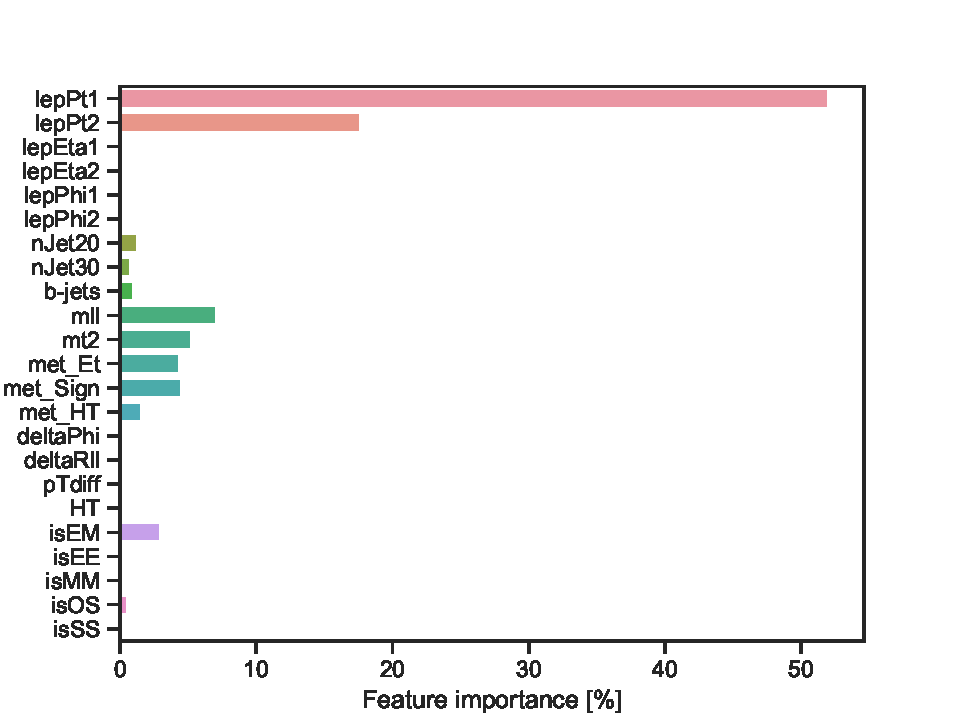
\includegraphics[width = \textwidth]{Figures/SlepSlep/ML/BDT/All_level/High/featureImportance.pdf}
        \caption{Direct slepton production.}
        \label{fig:featSlepslepHigh}
    \end{subfigure}
    \begin{subfigure}[t!]{0.49\textwidth}
        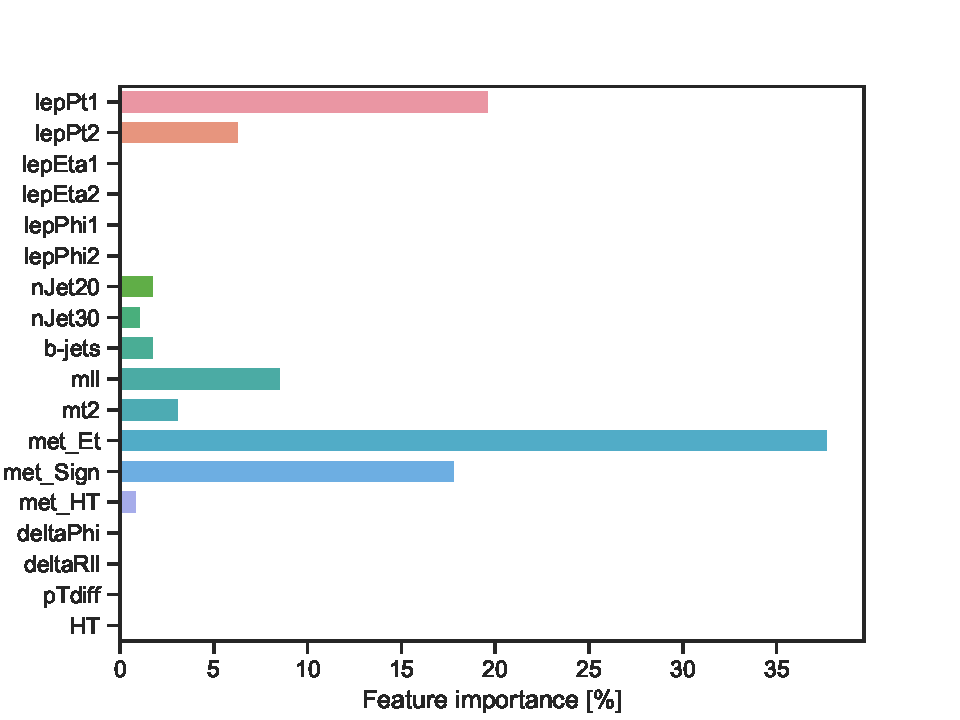
\includegraphics[width = \textwidth]{Figures/SlepSnu/BDT/All_level/High/featureImportance.pdf}
        \caption{Chargino production via $\Tilde{l}/\Tilde{\nu}$.}
        \label{fig:featSlepsnuHigh}
    \end{subfigure}
    \begin{subfigure}[t!]{0.49\textwidth}
        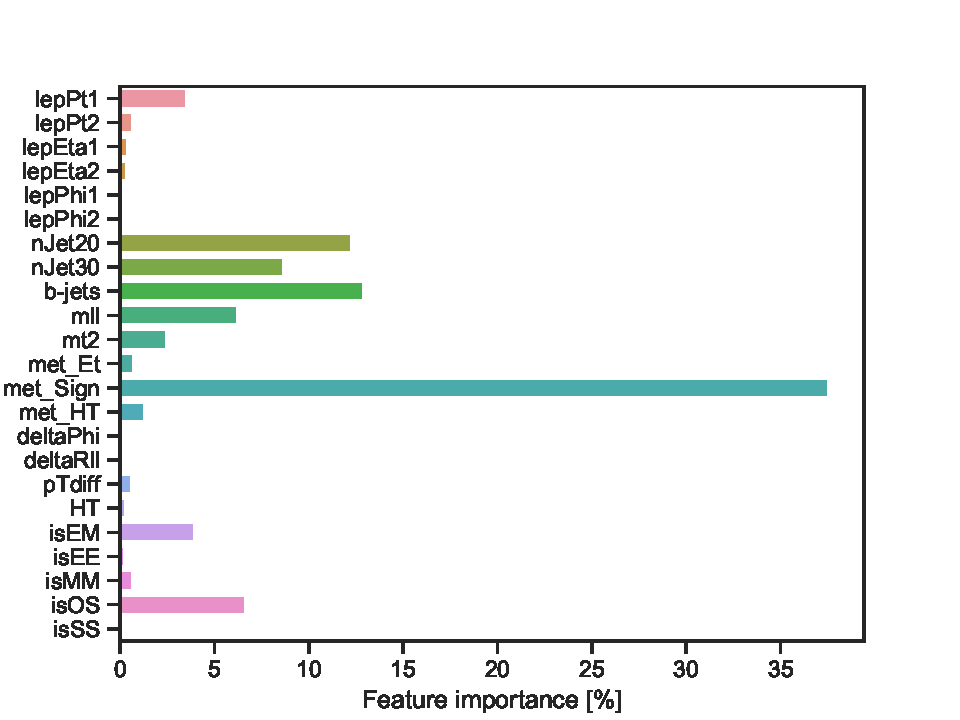
\includegraphics[width = \textwidth]{Figures/WW/BDT/All_level/High/featureImportance.pdf}
        \caption{Chargino production via $W^\pm$.}
        \label{fig:featWWHigh}
    \end{subfigure}
    \begin{subfigure}[t!]{0.49\textwidth}
        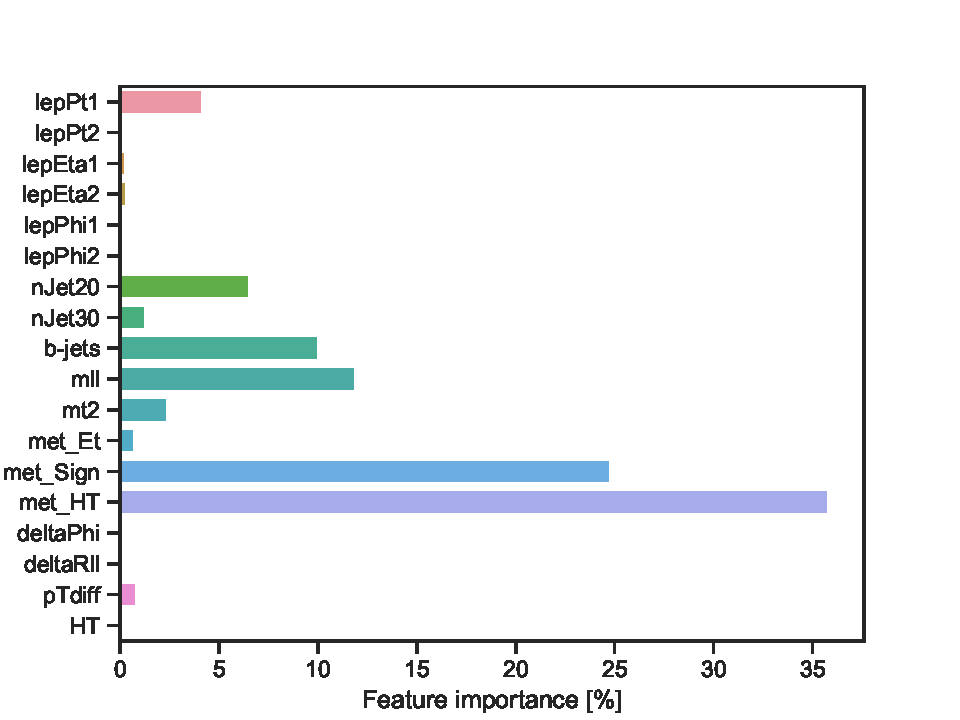
\includegraphics[width = \textwidth]{Figures/Mono_Z/ML/BDT/All_level/High/featureImportance.pdf}
        \caption{Mono-Z.}
        \label{fig:featMonoZHigh}
    \end{subfigure}
    \caption{Feature importance for high mass splittings for all four processes using all features during training.}
    \label{fig:AllHighfeatBDT}
\end{figure}

As we can see in figure \ref{fig:AllHighfeatBDT}, the momentum for the leading lepton have become a lot more interesting for the BDT especially for the direct slepton production. In addition the momentum for the subleading lepton have also gotten interesting for the two processes consisting sleptons. The rest of the features seems to be recurring for the processes no matter what mass splitting we look at. 



\begin{figure}[H]
    \centering
    \begin{subfigure}[t!]{0.49\textwidth}
        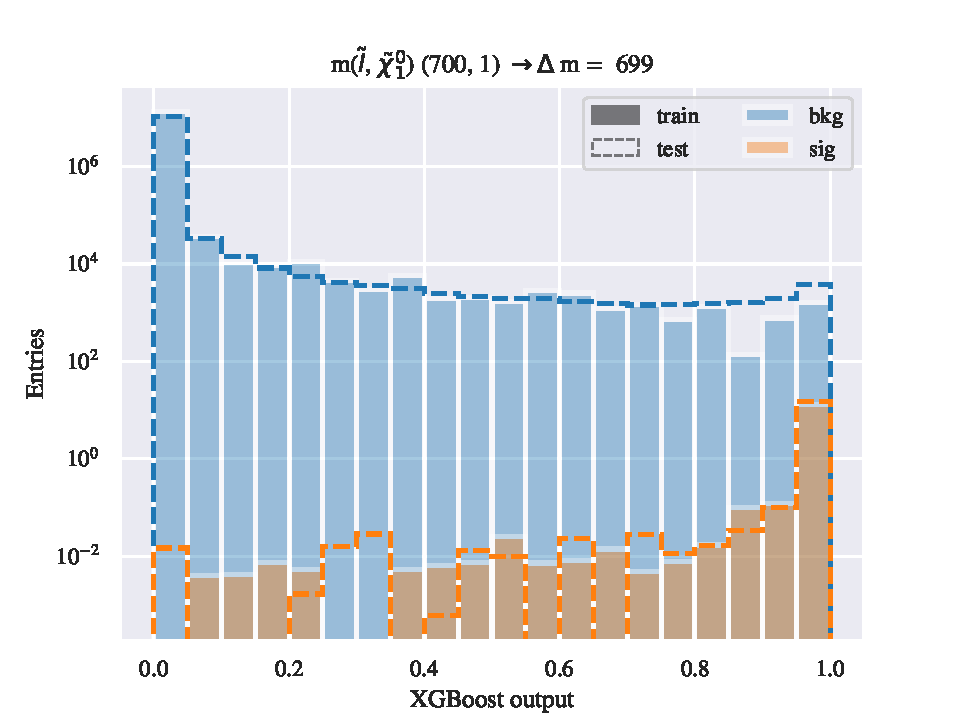
\includegraphics[width = \textwidth]{Figures/SlepSlep/ML/BDT/All_level/High/scaled_train_test_396033.pdf}
        \caption{Direct slepton production.}
        \label{fig:SlepslepHigh}
    \end{subfigure}
    \begin{subfigure}[t!]{0.49\textwidth}
        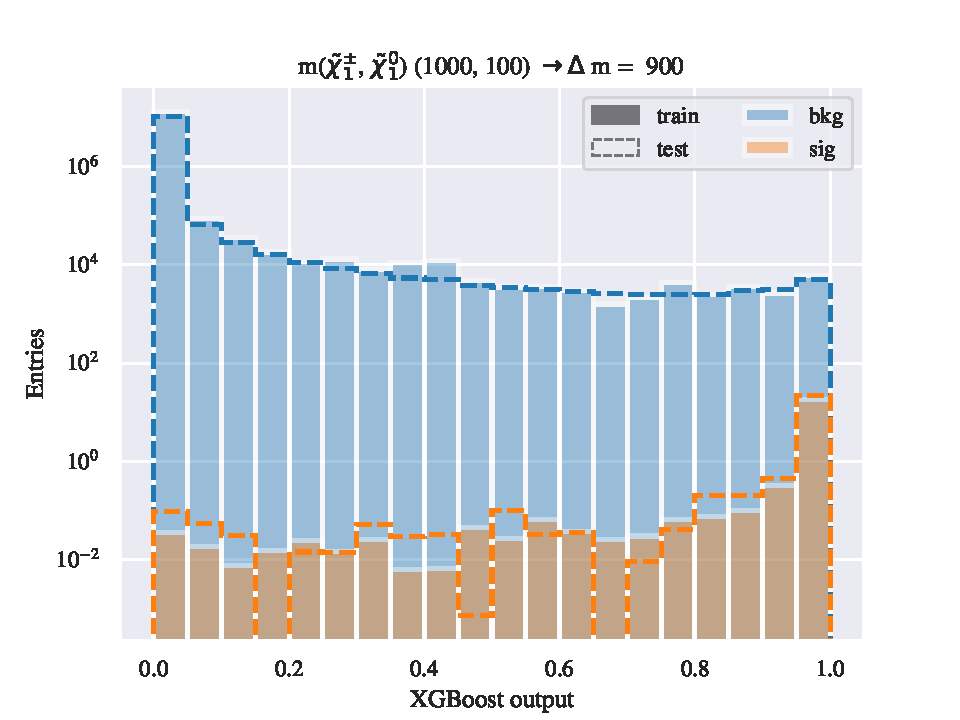
\includegraphics[width = \textwidth]{Figures/SlepSnu/BDT/All_level/High/scaled_train_test_397169.pdf}
        \caption{Chargino production via $\Tilde{l}/\Tilde{\nu}$.}
        \label{fig:SlepsnuHigh}
    \end{subfigure}
    \begin{subfigure}[t!]{0.49\textwidth}
        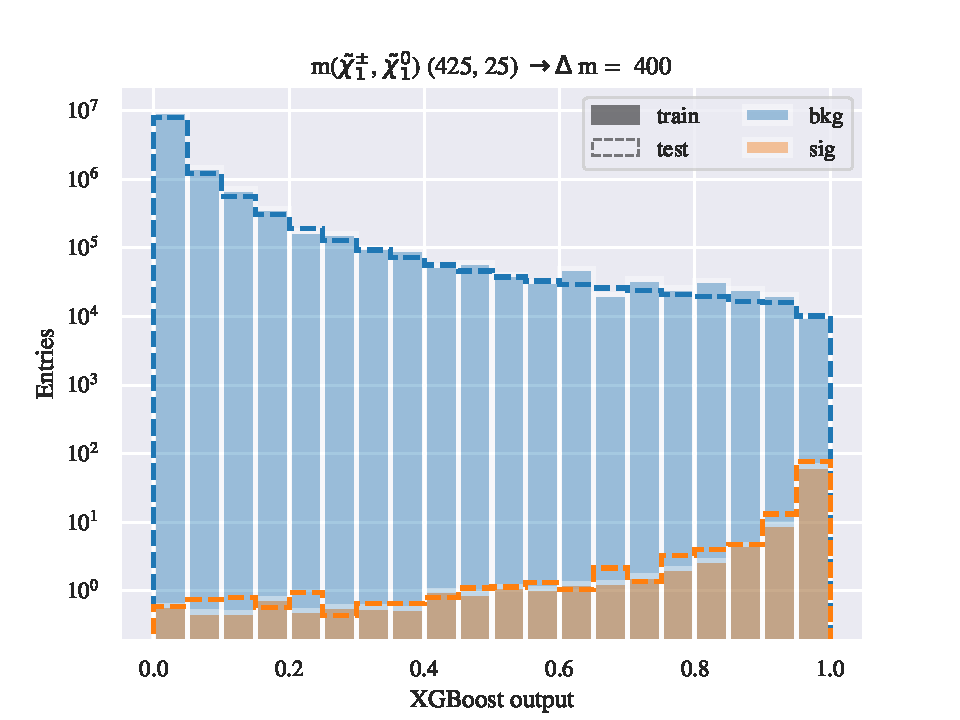
\includegraphics[width = \textwidth]{Figures/WW/BDT/All_level/High/scaled_train_test_395330.pdf}
        \caption{Chargino production via $W^\pm$.}
        \label{fig:WWHigh}
    \end{subfigure}
    \begin{subfigure}[t!]{0.49\textwidth}
        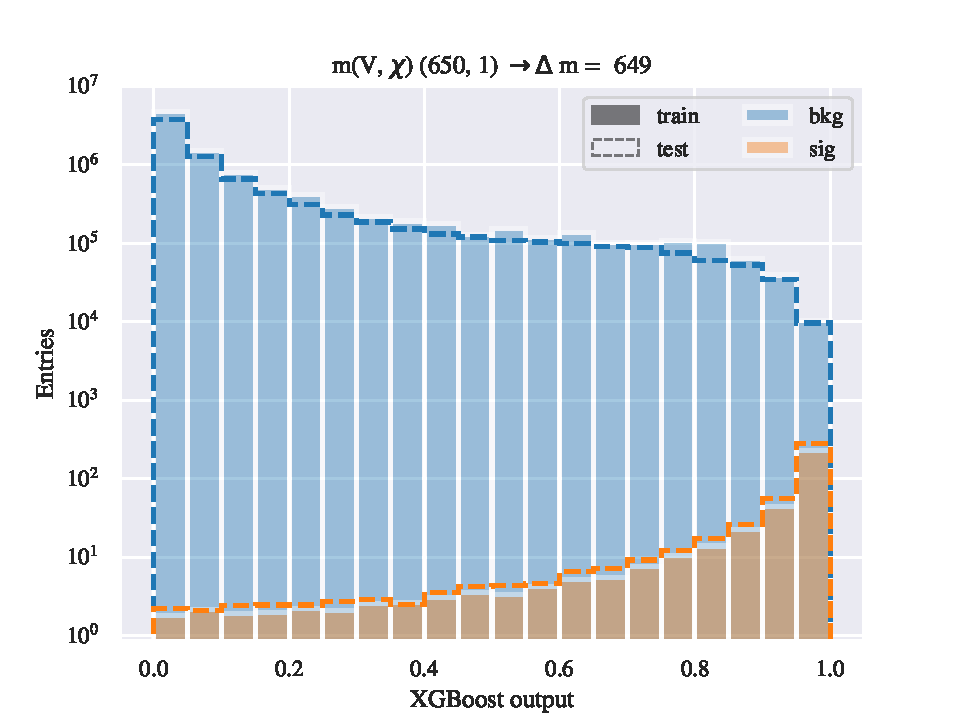
\includegraphics[width = \textwidth]{Figures/Mono_Z/ML/BDT/All_level/High/scaled_train_test_310617.pdf}
        \caption{Mono-Z.}
        \label{fig:MonoZHigh}
    \end{subfigure}
    \caption{Test vs train for high mass splittings done with the BDT. Here the test set is scaled up to match the number of training events.}
    \label{fig:AllHighBDT}
\end{figure}

In figure \ref{fig:AllHighBDT} we can see the results from testing our BDT. In figure \ref{fig:WWHigh} and \ref{fig:MonoZHigh} we can see that the match is overall pretty good, while for the processes in figure \ref{fig:SlepslepHigh} and \ref{fig:SlepsnuHigh} does not match that well. It can be many reasons for this happening like it have too little input data to perform a proper training, the features that are chosen might be bad for the process with this mass splitting, tendency to over/underfitting or that the parameters that have worked good for the rest is not right for this particular composition of mass splittings and features. Anyhow, it have succeeded better on classifying the signal and background. We can see for all four processes that we have more signal in the last bin than in any of the other models shown earlier in this chapter. This is of course not that surprising since these masses are outside of the SM masses we already know very well.



\subsubsection{Summarizing the BDT}
The BDT is in general performing good even though the separation of background and signal could be a bit better. 




\section{Building, training and testing the NN}\improvement{Kommentar til Mona: Begrunn hvorfor vi ikke har feature importance for NN og at man da må ta en sjans på hvilke som er best når AUC er lik for to modeller. Plott kommer i morgen :D :D :D}

In the following sections we are going to look at how the NN is built up, trained and tested before we in the end go to the last part of the ML where we are going to test the trained models on real data.

\subsection{Building}
As for the BDT, the NN uses some already existing libraries. The main parts of the building is covered in chapter \ref{sec:NN} and the parameters we us to optimize the NN is presented in table \ref{tab:parametersNN}.

\begin{table}[H]
    \centering
    \renewcommand{\arraystretch}{1.}
    \begin{tabular}{c c}
    \toprule
        \textbf{Parameter} & \textbf{Value}\\
        \midrule
        \midrule
        Number of nodes & 300  \\
        Number of hidden layers & 5\\
        Dropout rate & 0\\
        Batch size & 32\\
        Epochs & 100000\\
        Learning rate & $10^{-5}$\\
        L1 & 0\\
        L2 & $10^{-3}$\\
        \bottomrule
    \end{tabular}
    \caption{An overview of the different parameters used during training to obtain the results for the NN.}
    \label{tab:parametersNN}
\end{table}

Most of the parameters are very self explanatory, but we are going to go through them step by step so we are sure that we have understood every one of them. The first one is the number of nodes which is the number of nodes in each layer and not the total number in the network. Then we have the number of hidden layers which is the number of how many layers we want inside the network in addition to the input and output layer. Dropout rate is a number between 0 and 1 and is taken into consideration if you want to drop a percentage of your input when you start training. As we can see, we have not used the dropout rate other than telling our NN that it should not drop any of the input, so we are not going to go into the advantages or disadvantages with using this. The next parameter is the batch size which is the number of iterations we go through the data we give the NN. This can be any value above 1 but it is popular to set it to a number of power of 2. The epochs and learning rate should be clear from chapter \ref{sec:NN}, where the epochs is not a very interesting parameter due to the early stopping and the learning rate gets optimized by Adam. The last two parameters we have to take into consideration is L1 and L2, which is what we call \textit{layer weight regularizes}. These are applied to add a penalty on the layers kernel. 

\subsection{Training}

\subsection{Testing}












\subsubsection{AUC-score}

\begin{table}[H]
    \centering
    \renewcommand{\arraystretch}{1.}
    \begin{tabular}{l l c c c c }
    \toprule
    \textbf{Level} & $\mathbf{\Delta m}$ & $\mathbf{\Tilde{l} \Tilde{l}}$ & $\mathbf{\Tilde{\chi}_1^\pm \rightarrow \Tilde{l}/\Tilde{\nu}}$ & $\mathbf{\Tilde{\chi}_1^\pm \rightarrow W^\pm}$ & \textbf{Mono-Z}  \\
    \midrule
    \midrule
    \multirow{3}{*}{High} &  Low   & 0.92 & 0.91 & 0.91 & 0.95 \\
     & Intermediate & 0.99 & 0.97 & 0.94 & 0.96 \\
     & High & 1.00 & 1.00 & 0.96 & 0.97 \\
     \midrule
    \multirow{3}{*}{Low} & Low & 0.94 & 0.92 & 0.92 & 0.95 \\
     & Intermediate & 0.99 & 0.98 & 0.95 & 0.97 \\
     & High & 1.00 & 1.00 & 0.97 & 0.97 \\
     \midrule
    \multirow{3}{*}{All} & Low & 0.95 & 0.94 & 0.94 & 0.96 \\
     & Intermediate & 0.99 & 0.98 & 0.95 & 0.97 \\
     & High & 1.00 & 1.00 & 0.97 & 0.98 \\
     \bottomrule
    \end{tabular}
    \caption{The AUC score for the different processes trained on different compositions of features and mass splittings for the NN.}
    \label{tab:AUCNN}
\end{table}
%%%%%%%%%%%%%%%%%%%%%%%%%%%%%%%%%%%%%%%%%%%%%%%%%%%%%%






\subsubsection{Low mass splittings}
\begin{figure}[H]
    \centering
    \begin{subfigure}[t!]{0.49\textwidth}
        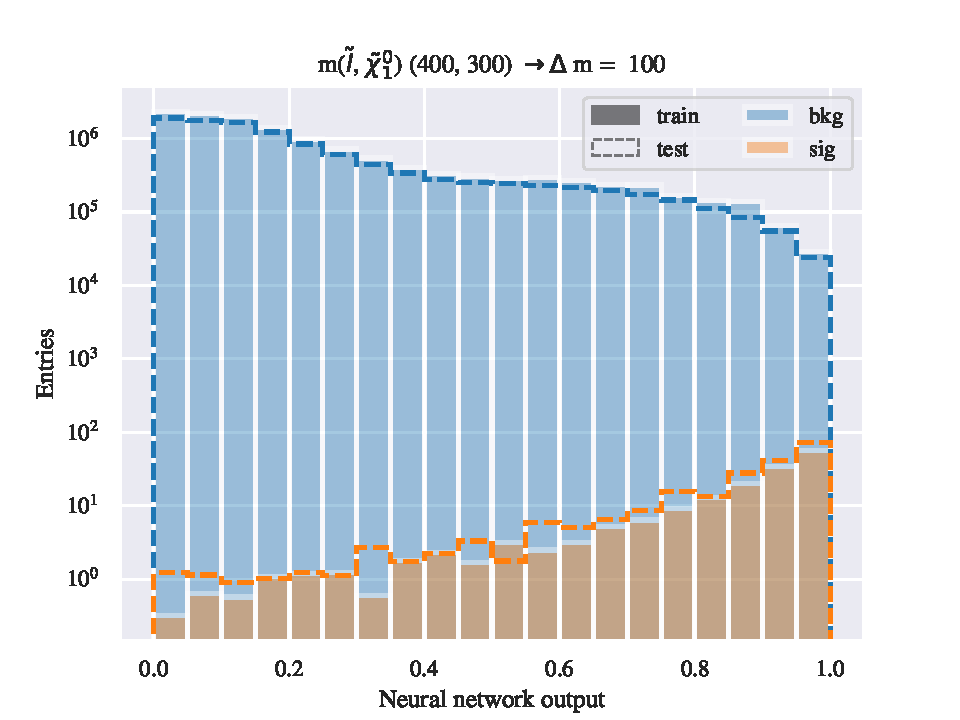
\includegraphics[width = \textwidth]{Figures/SlepSlep/ML/NN/Low_level/Low/scaled_train_test_395984.pdf}
        \caption{Direct slepton production.}
        \label{fig:SlepslepNNLow}
    \end{subfigure}
    \begin{subfigure}[t!]{0.49\textwidth}
        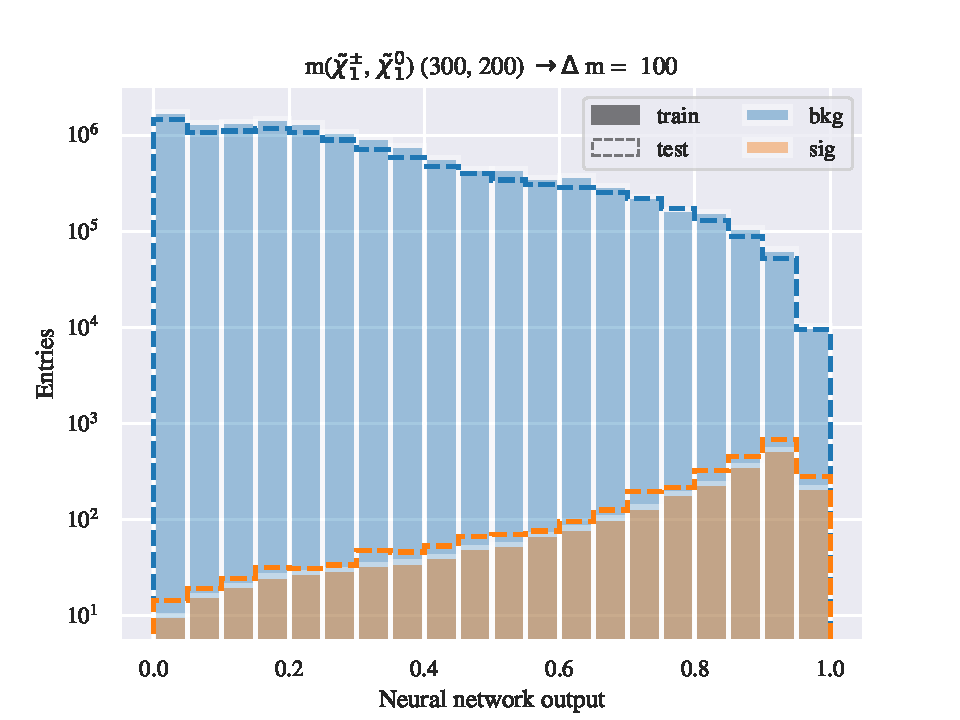
\includegraphics[width = \textwidth]{Figures/SlepSnu/NN/Low_level/Low/scaled_train_test_397115.pdf}
        \caption{Chargino production via $\Tilde{l}/\Tilde{\nu}$.}
        \label{fig:SlepsnuNNLow}
    \end{subfigure}    
    \begin{subfigure}[t!]{0.49\textwidth}
        \includegraphics[width = \textwidth]{Figures/WW/NN/Low_level/Low/scaled_train_test_395268.pdf}
        \caption{Chargino production via $W^\pm$.}
        \label{fig:WWNNLow}
    \end{subfigure}
    \begin{subfigure}[t!]{0.49\textwidth}
        \includegraphics[width = \textwidth]{Figures/Mono_Z/ML/NN/Low_level/Low/scaled_train_test_310604.pdf}
        \caption{Mono-Z.}
        \label{fig:MonoZNNLow}
    \end{subfigure}
    \caption{Test vs train for low mass splittings done with the NN. Here the test set is scaled up to match the number of training events.}
    \label{fig:AllLowNN}
\end{figure}


\begin{figure}[H]
    \centering
    \begin{subfigure}[t!]{0.49\textwidth}
        \includegraphics[width = \textwidth]{Figures/SlepSlep/ML/NN/High_level/Low/scaled_train_test_395984.pdf}
        \caption{Direct slepton production.}
        \label{fig:SlepslepNNLow}
    \end{subfigure}
    \begin{subfigure}[t!]{0.49\textwidth}
        \includegraphics[width = \textwidth]{Figures/SlepSnu/NN/High_level/Low/scaled_train_test_397115.pdf}
        \caption{Chargino production via $\Tilde{l}/\Tilde{\nu}$.}
        \label{fig:SlepsnuNNLow}
    \end{subfigure}    
    \begin{subfigure}[t!]{0.49\textwidth}
        \includegraphics[width = \textwidth]{Figures/WW/NN/High_level/Low/scaled_train_test_395268.pdf}
        \caption{Chargino production via $W^\pm$.}
        \label{fig:WWNNLow}
    \end{subfigure}
    \begin{subfigure}[t!]{0.49\textwidth}
        \includegraphics[width = \textwidth]{Figures/Mono_Z/ML/NN/High_level/Low/scaled_train_test_310604.pdf}
        \caption{Mono-Z.}
        \label{fig:MonoZNNLow}
    \end{subfigure}
    \caption{Test vs train for low mass splittings done with the NN. Here the test set is scaled up to match the number of training events.}
    \label{fig:AllLowNN}
\end{figure}


\begin{figure}[H]
    \centering
    \begin{subfigure}[t!]{0.49\textwidth}
        \includegraphics[width = \textwidth]{Figures/SlepSlep/ML/NN/All_level/Low/scaled_train_test_395984.pdf}
        \caption{Direct slepton production.}
        \label{fig:SlepslepNNLow}
    \end{subfigure}
    \begin{subfigure}[t!]{0.49\textwidth}
        \includegraphics[width = \textwidth]{Figures/SlepSnu/NN/All_level/Low/scaled_train_test_397115.pdf}
        \caption{Chargino production via $\Tilde{l}/\Tilde{\nu}$.}
        \label{fig:SlepsnuNNLow}
    \end{subfigure}    
    \begin{subfigure}[t!]{0.49\textwidth}
        \includegraphics[width = \textwidth]{Figures/WW/NN/All_level/Low/scaled_train_test_395268.pdf}
        \caption{Chargino production via $W^\pm$.}
        \label{fig:WWNNLow}
    \end{subfigure}
    \begin{subfigure}[t!]{0.49\textwidth}
        \includegraphics[width = \textwidth]{Figures/Mono_Z/ML/NN/All_level/Low/scaled_train_test_310604.pdf}
        \caption{Mono-Z.}
        \label{fig:MonoZNNLow}
    \end{subfigure}
    \caption{Test vs train for low mass splittings done with the NN. Here the test set is scaled up to match the number of training events.}
    \label{fig:AllLowNN}
\end{figure}














\subsubsection{Intermediate mass splittings}



\begin{figure}[H]
    \centering
    \begin{subfigure}[t!]{0.49\textwidth}
        \includegraphics[width = \textwidth]{Figures/SlepSlep/ML/NN/Low_level/Inter/scaled_train_test_396014.pdf}
        \caption{Direct slepton production.}
        \label{fig:SlepslepNNLow}
    \end{subfigure}
    \begin{subfigure}[t!]{0.49\textwidth}
        \includegraphics[width = \textwidth]{Figures/SlepSnu/NN/Low_level/Inter/scaled_train_test_397150.pdf}
        \caption{Chargino production via $\Tilde{l}/\Tilde{\nu}$.}
        \label{fig:SlepsnuNNLow}
    \end{subfigure}    
    \begin{subfigure}[t!]{0.49\textwidth}
        \includegraphics[width = \textwidth]{Figures/WW/NN/Low_level/Inter/scaled_train_test_395320.pdf}
        \caption{Chargino production via $W^\pm$.}
        \label{fig:WWNNLow}
    \end{subfigure}
    \begin{subfigure}[t!]{0.49\textwidth}
        \includegraphics[width = \textwidth]{Figures/Mono_Z/ML/NN/Low_level/Inter/scaled_train_test_310613.pdf}
        \caption{Mono-Z.}
        \label{fig:MonoZNNLow}
    \end{subfigure}
    \caption{Test vs train for low mass splittings done with the NN. Here the test set is scaled up to match the number of training events.}
    \label{fig:AllLowNN}
\end{figure}


\begin{figure}[H]
    \centering
    \begin{subfigure}[t!]{0.49\textwidth}
        \includegraphics[width = \textwidth]{Figures/SlepSlep/ML/NN/High_level/Inter/scaled_train_test_396014.pdf}
        \caption{Direct slepton production.}
        \label{fig:SlepslepNNLow}
    \end{subfigure}
    \begin{subfigure}[t!]{0.49\textwidth}
        \includegraphics[width = \textwidth]{Figures/SlepSnu/NN/High_level/Inter/scaled_train_test_397150.pdf}
        \caption{Chargino production via $\Tilde{l}/\Tilde{\nu}$.}
        \label{fig:SlepsnuNNLow}
    \end{subfigure}    
    \begin{subfigure}[t!]{0.49\textwidth}
        \includegraphics[width = \textwidth]{Figures/WW/NN/High_level/Inter/scaled_train_test_395320.pdf}
        \caption{Chargino production via $W^\pm$.}
        \label{fig:WWNNLow}
    \end{subfigure}
    \begin{subfigure}[t!]{0.49\textwidth}
        \includegraphics[width = \textwidth]{Figures/Mono_Z/ML/NN/High_level/Inter/scaled_train_test_310613.pdf}
        \caption{Mono-Z.}
        \label{fig:MonoZNNLow}
    \end{subfigure}
    \caption{Test vs train for low mass splittings done with the NN. Here the test set is scaled up to match the number of training events.}
    \label{fig:AllLowNN}
\end{figure}


\begin{figure}[H]
    \centering
    \begin{subfigure}[t!]{0.49\textwidth}
        \includegraphics[width = \textwidth]{Figures/SlepSlep/ML/NN/All_level/Inter/scaled_train_test_396014.pdf}
        \caption{Direct slepton production.}
        \label{fig:SlepslepNNLow}
    \end{subfigure}
    \begin{subfigure}[t!]{0.49\textwidth}
        \includegraphics[width = \textwidth]{Figures/SlepSnu/NN/All_level/Inter/scaled_train_test_397150.pdf}
        \caption{Chargino production via $\Tilde{l}/\Tilde{\nu}$.}
        \label{fig:SlepsnuNNLow}
    \end{subfigure}    
    \begin{subfigure}[t!]{0.49\textwidth}
        \includegraphics[width = \textwidth]{Figures/WW/NN/All_level/Inter/scaled_train_test_395320.pdf}
        \caption{Chargino production via $W^\pm$.}
        \label{fig:WWNNLow}
    \end{subfigure}
    \begin{subfigure}[t!]{0.49\textwidth}
        \includegraphics[width = \textwidth]{Figures/Mono_Z/ML/NN/All_level/Inter/scaled_train_test_310613.pdf}
        \caption{Mono-Z.}
        \label{fig:MonoZNNLow}
    \end{subfigure}
    \caption{Test vs train for low mass splittings done with the NN. Here the test set is scaled up to match the number of training events.}
    \label{fig:AllLowNN}
\end{figure}



















\subsubsection{High mass splittings}

\begin{figure}[H]
    \centering
    \begin{subfigure}[t!]{0.49\textwidth}
        \includegraphics[width = \textwidth]{Figures/SlepSlep/ML/NN/Low_level/High/scaled_train_test_396033.pdf}
        \caption{Direct slepton production.}
        \label{fig:SlepslepNNLow}
    \end{subfigure}
    \begin{subfigure}[t!]{0.49\textwidth}
        \includegraphics[width = \textwidth]{Figures/SlepSnu/NN/Low_level/High/scaled_train_test_397169.pdf}
        \caption{Chargino production via $\Tilde{l}/\Tilde{\nu}$.}
        \label{fig:SlepsnuNNLow}
    \end{subfigure}    
    \begin{subfigure}[t!]{0.49\textwidth}
        \includegraphics[width = \textwidth]{Figures/WW/NN/Low_level/High/scaled_train_test_395330.pdf}
        \caption{Chargino production via $W^\pm$.}
        \label{fig:WWNNLow}
    \end{subfigure}
    \begin{subfigure}[t!]{0.49\textwidth}
        \includegraphics[width = \textwidth]{Figures/Mono_Z/ML/NN/Low_level/High/scaled_train_test_310617.pdf}
        \caption{Mono-Z.}
        \label{fig:MonoZNNLow}
    \end{subfigure}
    \caption{Test vs train for low mass splittings done with the NN. Here the test set is scaled up to match the number of training events.}
    \label{fig:AllLowNN}
\end{figure}


\begin{figure}[H]
    \centering
    \begin{subfigure}[t!]{0.49\textwidth}
        \includegraphics[width = \textwidth]{Figures/SlepSlep/ML/NN/High_level/High/scaled_train_test_396033.pdf}
        \caption{Direct slepton production.}
        \label{fig:SlepslepNNLow}
    \end{subfigure}
    \begin{subfigure}[t!]{0.49\textwidth}
        \includegraphics[width = \textwidth]{Figures/SlepSnu/NN/High_level/High/scaled_train_test_397169.pdf}
        \caption{Chargino production via $\Tilde{l}/\Tilde{\nu}$.}
        \label{fig:SlepsnuNNLow}
    \end{subfigure}    
    \begin{subfigure}[t!]{0.49\textwidth}
        \includegraphics[width = \textwidth]{Figures/WW/NN/High_level/High/scaled_train_test_395330.pdf}
        \caption{Chargino production via $W^\pm$.}
        \label{fig:WWNNLow}
    \end{subfigure}
    \begin{subfigure}[t!]{0.49\textwidth}
        \includegraphics[width = \textwidth]{Figures/Mono_Z/ML/NN/High_level/High/scaled_train_test_310617.pdf}
        \caption{Mono-Z.}
        \label{fig:MonoZNNLow}
    \end{subfigure}
    \caption{Test vs train for low mass splittings done with the NN. Here the test set is scaled up to match the number of training events.}
    \label{fig:AllLowNN}
\end{figure}


\begin{figure}[H]
    \centering
    \begin{subfigure}[t!]{0.49\textwidth}
        \includegraphics[width = \textwidth]{Figures/SlepSlep/ML/NN/All_level/High/scaled_train_test_396033.pdf}
        \caption{Direct slepton production.}
        \label{fig:SlepslepNNLow}
    \end{subfigure}
    \begin{subfigure}[t!]{0.49\textwidth}
        \includegraphics[width = \textwidth]{Figures/SlepSnu/NN/All_level/High/scaled_train_test_397169.pdf}
        \caption{Chargino production via $\Tilde{l}/\Tilde{\nu}$.}
        \label{fig:SlepsnuNNLow}
    \end{subfigure}    
    \begin{subfigure}[t!]{0.49\textwidth}
        \includegraphics[width = \textwidth]{Figures/WW/NN/All_level/High/scaled_train_test_395330.pdf}
        \caption{Chargino production via $W^\pm$.}
        \label{fig:WWNNLow}
    \end{subfigure}
    \begin{subfigure}[t!]{0.49\textwidth}
        \includegraphics[width = \textwidth]{Figures/Mono_Z/ML/NN/All_level/High/scaled_train_test_310617.pdf}
        \caption{Mono-Z.}
        \label{fig:MonoZNNLow}
    \end{subfigure}
    \caption{Test vs train for low mass splittings done with the NN. Here the test set is scaled up to match the number of training events.}
    \label{fig:AllLowNN}
\end{figure}



















\section{Testing the BDT and NN on real data}



\begin{figure}[H]
    \centering
        \includegraphics[width = \textwidth]{Figures/Stacked/stackedplot_BDT_All_level_slepslep.pdf}
        \caption{}
        \label{fig:traintestscaled}
\end{figure}

\begin{figure}[H]
    \centering
        \includegraphics[width = \textwidth]{Figures/Stacked/stackedplot_BDT_Low_level_slepslep.pdf}
        \caption{}
        \label{fig:traintestscaled}
\end{figure}

\begin{figure}[H]
    \centering
        \includegraphics[width = \textwidth]{Figures/Stacked/stackedplot_BDT_High_level_slepslep.pdf}
        \caption{}
        \label{fig:traintestscaled}
\end{figure}





\begin{figure}[H]
    \centering
        \includegraphics[width = \textwidth]{Figures/Stacked/stackedplot_BDT_All_level_slepsnu.pdf}
        \caption{}
        \label{fig:traintestscaled}
\end{figure}

\begin{figure}[H]
    \centering
        \includegraphics[width = \textwidth]{Figures/Stacked/stackedplot_BDT_Low_level_slepsnu.pdf}
        \caption{}
        \label{fig:traintestscaled}
\end{figure}

\begin{figure}[H]
    \centering
        \includegraphics[width = \textwidth]{Figures/Stacked/stackedplot_BDT_High_level_slepsnu.pdf}
        \caption{}
        \label{fig:traintestscaled}
\end{figure}








\begin{figure}[H]
    \centering
        \includegraphics[width = \textwidth]{Figures/Stacked/stackedplot_BDT_All_level_WW.pdf}
        \caption{}
        \label{fig:traintestscaled}
\end{figure}

\begin{figure}[H]
    \centering
        \includegraphics[width = \textwidth]{Figures/Stacked/stackedplot_BDT_Low_level_WW.pdf}
        \caption{}
        \label{fig:traintestscaled}
\end{figure}

\begin{figure}[H]
    \centering
        \includegraphics[width = \textwidth]{Figures/Stacked/stackedplot_BDT_High_level_WW.pdf}
        \caption{}
        \label{fig:traintestscaled}
\end{figure}





\begin{figure}[H]
    \centering
        \includegraphics[width = \textwidth]{Figures/Stacked/stackedplot_BDT_All_level_monoZ.pdf}
        \caption{}
        \label{fig:traintestscaled}
\end{figure}

\begin{figure}[H]
    \centering
        \includegraphics[width = \textwidth]{Figures/Stacked/stackedplot_BDT_Low_level_monoZ.pdf}
        \caption{}
        \label{fig:traintestscaled}
\end{figure}

\begin{figure}[H]
    \centering
        \includegraphics[width = \textwidth]{Figures/Stacked/stackedplot_BDT_High_level_monoZ.pdf}
        \caption{}
        \label{fig:traintestscaled}
\end{figure}

























\begin{figure}[H]
    \centering
        \includegraphics[width = \textwidth]{Figures/Stacked/stackedplot_NN_All_level_slepslep.pdf}
        \caption{}
        \label{fig:traintestscaled}
\end{figure}

\begin{figure}[H]
    \centering
        \includegraphics[width = \textwidth]{Figures/Stacked/stackedplot_NN_Low_level_slepslep.pdf}
        \caption{}
        \label{fig:traintestscaled}
\end{figure}

\begin{figure}[H]
    \centering
        \includegraphics[width = \textwidth]{Figures/Stacked/stackedplot_NN_High_level_slepslep.pdf}
        \caption{}
        \label{fig:traintestscaled}
\end{figure}





\begin{figure}[H]
    \centering
        \includegraphics[width = \textwidth]{Figures/Stacked/stackedplot_NN_All_level_slepsnu.pdf}
        \caption{}
        \label{fig:traintestscaled}
\end{figure}

\begin{figure}[H]
    \centering
        \includegraphics[width = \textwidth]{Figures/Stacked/stackedplot_NN_Low_level_slepsnu.pdf}
        \caption{}
        \label{fig:traintestscaled}
\end{figure}

\begin{figure}[H]
    \centering
        \includegraphics[width = \textwidth]{Figures/Stacked/stackedplot_NN_High_level_slepsnu.pdf}
        \caption{}
        \label{fig:traintestscaled}
\end{figure}








\begin{figure}[H]
    \centering
        \includegraphics[width = \textwidth]{Figures/Stacked/stackedplot_NN_All_level_WW.pdf}
        \caption{}
        \label{fig:traintestscaled}
\end{figure}

\begin{figure}[H]
    \centering
        \includegraphics[width = \textwidth]{Figures/Stacked/stackedplot_NN_Low_level_WW.pdf}
        \caption{}
        \label{fig:traintestscaled}
\end{figure}

\begin{figure}[H]
    \centering
        \includegraphics[width = \textwidth]{Figures/Stacked/stackedplot_NN_High_level_WW.pdf}
        \caption{}
        \label{fig:traintestscaled}
\end{figure}





\begin{figure}[H]
    \centering
        \includegraphics[width = \textwidth]{Figures/Stacked/stackedplot_NN_All_level_monoZ.pdf}
        \caption{}
        \label{fig:traintestscaled}
\end{figure}

\begin{figure}[H]
    \centering
        \includegraphics[width = \textwidth]{Figures/Stacked/stackedplot_NN_Low_level_monoZ.pdf}
        \caption{}
        \label{fig:traintestscaled}
\end{figure}

\begin{figure}[H]
    \centering
        \includegraphics[width = \textwidth]{Figures/Stacked/stackedplot_NN_High_level_monoZ.pdf}
        \caption{}
        \label{fig:traintestscaled}
\end{figure}



























\begin{comment}





These cuts are done in a script called \texttt{importdata.py} where you also set up all of the data (both MC and real data) in pandas dataframes \footnote{Pandas dataframes \cite{PD} is a two-dimensional frame of your data which also includes the corresponding labels.}. In this script you will find a function called \texttt{prepareInput} which will read in all of the data in chunks because reading in all of it at once is too much for the computer to handle. After reading in one chunk, the root files will be set up in Pandas dataframes before it is sent into the precuts function called \texttt{importData}. Then we shuffle all of the events in each chunk before we send it in to the function called \texttt{selectFeatures} where we select the features we want to have for our training in the ML algorithm. The features I chose for the direct slepton production is given in table \ref{tab:features}.



The next step is to get the event weights in the function \texttt{getEventWeights} where we weight each event depending on the different weights listed in table \ref{tab:eventWeights} and the luminosity which is 58.5 fb$^{(-1)}$ in our case.



And in the end it stores the preprocessed data in HDF5 files before it starts on a new chunk and do the process described above continuously until we have reached the end of the dataset. HDF5 \cite{hdf5} is a file format to store large, complex and heterogeneous data which we use to store our events temporarily to save some time so we don't have to do this part every time we are training a ML model. This is also a time consuming step of the code. All of this can be run by simply running \texttt{main.py} with some arguments. If you are going to do the preprocessing you can add \texttt{--prepare\_hdf5} as argument and if you want to do it for signal (\texttt{--sig}), background (\texttt{--bkg}) and data (\texttt{--data}). I have also divided the signal samples into low, intermediate and high mass splitting to get more statistics from the training and testing. This means if you are going to do this for signal you have to add an argument \texttt{--low}, \texttt{--inter} or \texttt{--high}, where low is $\Delta m < 100$GeV, intermediate is $100$GeV $\leq \Delta m < 450$GeV and high is $\Delta m \geq 450$GeV. Which signal samples that are in which "group", you can see in table \ref{tab:directslepLOW}, \ref{tab:directslepINTER1}, \ref{tab:directslepINTER2} and \ref{tab:directslepHIGH} in section \ref{sec:sigsamptab}.

The next step is to do the actual ML which can be done by running the script \texttt{main.py} with some new arguments. The first thing you want to do is to read in the HDF5 files we made in the previous part which is simply done by adding \texttt{--read\_hdf5} as an argument. You also have to choose if you wanna train the model on low, intermediate mass splitting which is done by adding \texttt{--sig} and one of the following arguments \texttt{--low}, \texttt{--inter} or \texttt{--high}. You also have to choose which model you wanna train where you add either \texttt{--xgboost} for running XGBoost or \texttt{--nn} to run the neural network. If you run with all of this arguments you will train a new model. If you don't want to train a new model and just use a earlier trained model you can simply add \texttt{--load\_pretrained\_model} and it will use a pretrained model instead. This is mostly used to see how our model are doing compared to real data. To do this you have to read the hdf5 files, load the pretrained model, tell if you want the low, intermediate or high version and that you want data, which is done by simply adding the argument \texttt{--data}. 


\end{comment}










\begin{comment}



\begin{figure}[H]
%\begin{minipage}{2\textwidth}
%\begin{adjustwidth}{-3cm}{-3cm}
\centering
%\advance\leftskip-4cm 
%\advance\rightskip-4cm 
    \begin{subfloat}[][a]
        \includegraphics{Figures/SlepSlep/CutAndCount/ML_cuts/hist1d_mll_ML_cuts.pdf}
    \caption{Invariant mass.}
    \label{fig:my_label}
    \end{subfloat}
    \begin{subfloat}[t!]{0.49\textwidth}
        \includegraphics[width=\textwidth]{Figures/SlepSlep/CutAndCount/ML_cuts/hist1d_met_Et_ML_cuts.pdf}
    \caption{Missing transverse energy.}
    \label{fig:my_label}
    \end{subfloat}
    \\
    \begin{subfloat}[t!]{0.49\textwidth}
        \includegraphics[width=\textwidth]{Figures/SlepSlep/CutAndCount/ML_cuts/hist1d_mt2_ML_cuts.pdf}
    \caption{Stransverse mass.}
    \label{fig:my_label}
    \end{subfloat}
    \begin{subfloat}[t!]{0.49\textwidth}
        \includegraphics[width=\textwidth]{Figures/SlepSlep/CutAndCount/ML_cuts/hist1d_nBJet20_MV2c10_FixedCutBEff_77_ML_cuts.pdf}
    \caption{B-jets.}
    \label{fig:my_label}
    \end{subfloat}
    \\
    \begin{subfloat}[t!]{0.49\textwidth}
        \includegraphics[width=\textwidth]{Figures/SlepSlep/CutAndCount/ML_cuts/hist1d_nJet20_ML_cuts.pdf}
    \caption{Jets with $p_T > 20$GeV.}
    \label{fig:my_label}
    \end{subfloat}
    \begin{subfloat}[t!]{0.49\textwidth}
        \includegraphics[width=\textwidth]{Figures/SlepSlep/CutAndCount/ML_cuts/hist1d_nJet30_ML_cuts.pdf}
    \caption{Jets with $p_T > 30$GeV.}
    \label{fig:my_label}
    \end{subfloat}
    \\
    \begin{subfloat}[t!]{0.49\textwidth}
        \includegraphics[width=\textwidth]{Figures/SlepSlep/CutAndCount/ML_cuts/hist1d_lepPt[0]_ML_cuts.pdf}
    \caption{The transverse momentum for lepton 1.}
    \label{fig:my_label}
    \end{subfloat}
    \begin{subfloat}[t!]{0.49\textwidth}
        \includegraphics[width=\textwidth]{Figures/SlepSlep/CutAndCount/ML_cuts/hist1d_lepPt[1]_ML_cuts.pdf}
   \caption{The transverse momentum for lepton 2.}
   \label{fig:my_label}
    \end{subfloat}
    \\
    \begin{subfloat}[t!]{0.49\textwidth}
        \includegraphics[width=\textwidth]{Figures/SlepSlep/CutAndCount/ML_cuts/hist1d_lepPt_ML_cuts.pdf}
    \caption{The total transverse momentum for both leptons.}
    \label{fig:my_label}
    \end{subfloat}
    \begin{subfloat}[t!]{0.49\textwidth}
        \includegraphics[width=\textwidth]{Figures/SlepSlep/CutAndCount/ML_cuts/hist1d_pTdiff_ML_cuts.pdf}
    \caption{The absolute difference between the dilepton $p_T$, the selected jets $p_T$ and the vector sum of $\Vec{E}_T^{miss}$.}
    \label{fig:my_label}
    \end{subfloat}
    \\
    \begin{subfloat}[t!]{0.49\textwidth}
        \includegraphics[width=\textwidth]{Figures/SlepSlep/CutAndCount/ML_cuts/hist1d_deltaRll_ML_cuts.pdf}
    \caption{Distance between the two leptons.}
    \label{fig:my_label}
    \end{subfloat}
    \begin{subfloat}[t!]{0.49\textwidth}
        \includegraphics[width=\textwidth]{Figures/SlepSlep/CutAndCount/ML_cuts/hist1d_deltaPhi_ML_cuts.pdf}
    \caption{The azimuthal angle difference between the dilepton system and $E_T^{miss}$.}
    \label{fig:my_label}
    \end{subfloat}
\end{figure}

\begin{figure}[H]
%\begin{minipage}{2\textwidth}
%\begin{adjustwidth}{-3cm}{-3cm}
\centering
    \begin{subfigure}[t!]{0.49\textwidth}
        \includegraphics[width=\textwidth]{Figures/SlepSlep/CutAndCount/ML_cuts/hist1d_HT_ML_cuts.pdf}
    \caption{The scalar sum of the $p_T$ of the selected jets and leptons.}
    \label{fig:my_label}
    \end{subfigure}
    \begin{subfigure}[t!]{0.49\textwidth}
        \includegraphics[width=\textwidth]{Figures/SlepSlep/CutAndCount/ML_cuts/hist1d_met_HT_ML_cuts.pdf}
    \caption{}
    \label{fig:my_label}
    \end{subfigure}
    
%\end{adjustwidth}
\end{figure}


\end{comment}












FOR NN USING RELU FOR INPUT AND HIDDEN LAYERS OG SIGMOID FOR OUTPUT LAYER